\documentclass[
11pt, english, singlespacing,
headsepline,
chapterinoneline,
%consistentlayout, 
]{MastersDoctoralThesis}

% Load packages
\usepackage[utf8]{inputenc} % Required for inputting international characters
\usepackage{fontenc} % Output font encoding for international characters
\usepackage{mathpazo} % Use the Palatino font by default
\usepackage[backend=bibtex,style=numeric,natbib=true]{biblatex} % Use the bibtex backend with the authoryear citation style (which resembles APA)

\addbibresource{Bibliography/bibliography.bib} % The filename of the bibliography

\usepackage[autostyle=true]{csquotes} % Required to generate language-dependent quotes in the bibliography



\usepackage{graphicx}
\usepackage{verbatim}
\usepackage{latexsym}
\usepackage{setspace}
\usepackage{float}
\usepackage{subcaption}
\usepackage{url}
\usepackage{hyperref}
\hypersetup{
     colorlinks=true,
     linkcolor=black,
     filecolor=black,
     citecolor=black,
     urlcolor=black,
}     
\usepackage{tabularx}
\usepackage{booktabs}
\usepackage{multirow}
\usepackage[normalem]{ulem}
\usepackage{pdfpages}
\usepackage[htt]{hyphenat}
\usepackage[acronym]{glossaries}
\usepackage{enumitem}
\usepackage{amsmath}
\usepackage{changepage}

\usepackage{pgfplots}
\usepackage{pgfplotstable}
\usepackage{siunitx}
\usepackage{tikz}

\usepackage{array}
\usetikzlibrary{positioning}
\pgfplotsset{compat=1.18}


% Margins
\geometry{
	paper=a4paper, % Change to letterpaper for US letter
	inner=2.5cm, % Inner margin
	outer=3.8cm, % Outer margin
	bindingoffset=.5cm, % Binding offset
	top=1.5cm, % Top margin
	bottom=1.5cm, % Bottom margin
	%showframe, % Uncomment to show how the type block is set on the page
}

% Information
\newcommand{\thesistype}{Master Thesis}
\newcommand{\titel}{Nonlinear Material Parameter Identification of Soft Materials Based on an Inverse Finite Element Method Approach}
\newcommand{\autor}{Nadia Pinedo Oruna, B.Sc.}
\newcommand{\matnumber}{397\,011}
\newcommand{\studyprogram}{General Mechanical Engineering M.Sc.}
\newcommand{\supervisorinternal}{Rasul Abdulsalamov, M.Sc.}
\newcommand{\supervisorexternal}{Prof. Kazumi Matsui}
\newcommand{\submitdate}{26\textsuperscript{th} of May 2023}




\begin{document}

\frontmatter % Use roman page numbering style (i, ii, iii, iv...) for the pre-content pages

\pagestyle{plain} % Default to the plain heading style until the thesis style is called for the body content

% Title page
\begin{titlepage}
	
	\begin{center}
		
		\vspace*{-2cm}
		\begin{minipage}[b]{0.45\textwidth}
		\end{minipage}
		\hfill
		\begin{minipage}[b]{0.45\textwidth}
		\begin{flushright}
					
\includegraphics[height=6em]{Style/rwth_km_logo_en.eps}
		\end{flushright}
		\end{minipage}
		
		\normalsize{\scshape{
				The present work was submitted to the Department of Continuum Mechanics}
		}\\[1em]
		\vspace{1cm}
		\normalsize{\scshape\textbf{Rheinisch-Westfälische Technische Hochschule Aachen}}\\
		\normalsize{\normalfont\scshape{Faculty of Mechanical Engineering}}
		
		
		\vspace{2cm}
		
		\Large{\scshape\textbf{\thesistype}}\\[4ex]
		\huge{\scshape\textbf{\titel}}\\[1.5ex]
		
		\vfill{}
		
		\normalsize
		\begin{tabular}{p{5cm}p{8cm}}
			Presented by: 			& \quad  \autor\\[1.2ex]
			Study programme:		& \quad  \\[1.2ex]
			Matriculation number: 	& \quad \matnumber\\[1.2ex]
			Reviewer: 				& \quad Univ.-Prof. Dr.-Ing. Mikhail Itskov\\[1.2ex]
			Supervisor:				& \quad \supervisorinternal \\[1.2ex]
			External supervisor:	& \quad \supervisorexternal \\[1.2ex]
		\end{tabular}
		
		\vspace{3cm}
		
		Aachen, \submitdate
		
		\vspace*{-3.3cm}
		
	\end{center}
	
\end{titlepage}
\newpage


% Declaration page
\begin{declaration}

I declare that this work has been composed by myself, and describes my own work, unless otherwise acknowledged in the text. 

All sentences or passages quoted in this paper from other people's work have been specifically acknowledged by clear cross-referencing to author, work and 
page(s). Any photos and illustrations which are not the work of the author have been used with the explicit permission of the originator and are specifically acknowledged. 

This work has not been and will not be submitted for any other degree or the obtaining of ECTS points at the RWTH Aachen University or any other institution of higher education.\\[1em]

Aachen, \submitdate \\[2em]

\begin{flushright}
	\line(1,0){200}\\
	\autor
\end{flushright}


\end{declaration}

\cleardoublepage


% Abstract
%\begin{abstract}
\addchaptertocentry{\abstractname} % Add the abstract to the table of contents
The Thesis Abstract is written here (and usually kept to just this page). The page is kept centered vertically so can expand into the blank space above the title too\ldots
\end{abstract}


% Acknowledgements
%\begin{acknowledgements}
\addchaptertocentry{\acknowledgementname} % Add the acknowledgements to the table of contents
I am profoundly grateful to everyone who has provide me assistance and support 
throughout these years to achieve the completion of my master thesis.\\

First of all, my deepest appreciation extends to Prof. Matsui and Prof. 
Yamada from Yokohama National University. The opportunity to collaborate with you on this project has 
been invaluable, and your unwavering guidance and support, both in Japan and Germany despite the 
distance, have been instrumental to my success.
I would also like to thank my supervisor, Rasul Abdulsalamov, whose effective supervision,
motivational encouragement, and consistent cooperation have been essential from start to the finish.

Likewise, I am equally indebted to my colleagues at YNU, particularly Yuta Mori, Chikako Natsumeda, and Yuuki Fukutani, 
whose full cooperation and support, even in the face of language barriers. I am deeply appreciative of their hard work and dedication.\\

My heartfelt thanks go to my husband, Stephan Stahlmann. His constant presence, emotional support, 
and encouragement on every step towards my goal meant everything to me.

I am also grateful to my parents, Ciro Pinedo and Nora Oruna, and my sister, Nathaly Pinedo, 
for their unwavering support from Peru and for always believing in me. 
Furthermore, I would like to thank my host parents, Karin and Ivano Rinaldo, and my 
extended family, the Stahlmann family. Their wishes for my success and comfort during challenging times have been
a source of strength.\\

Lastly, I would like to mention my friends: Johanna Müller, Andrea Toledo, Azusa Soejima, Dominik Horn,
Lisa Kahler, Andrés Splendido, Josefine Dannenberg and Alonso López.
Their assistance, time and kindness during the course of this
thesis have been a tremendous help.\\

Muchas gracias a todos.

\end{acknowledgements}


%	Include table content, list of figures and of tables
\tableofcontents % Prints the main table of contents

\listoffigures % Prints the list of figures

\listoftables % Prints the list of tables


% List of symbols, abbreviations and constants
%----------------------------------------------------------------------------------------
%	ABBREVIATIONS
%----------------------------------------------------------------------------------------

\begin{abbreviations}{ll} % Include a list of abbreviations (a table of two columns)

\textbf{FEA} & \textbf{F}inite \textbf{E}lement \textbf{A}nalysis\\
\textbf{FEM} & \textbf{F}inite \textbf{E}lement \textbf{M}ethod\\
\textbf{iFEM} & \textbf{i}nverse \textbf{F}inite \textbf{E}lement \textbf{M}ethod\\
\textbf{ASME} & (The) \textbf{A}merican \textbf{S}ociety (of) \textbf{M}echanical \textbf{E}ngineering\\
\textbf{TSSA} & \textbf{T}ransparent \textbf{S}tructural \textbf{S}ilicone \textbf{A}dhesive\\
\textbf{PDMS} & \textbf{P}oly\textbf{D}i\textbf{M}ethyl\textbf{S}iloxane\\
\textbf{MAS} & \textbf{M}inimal \textbf{A}ccess \textbf{S}urgery\\
\textbf{FE} & \textbf{F}inite \textbf{E}lement\\
\textbf{NH} & \textbf{N}eo-\textbf{H}ookean\\
\textbf{MR} & \textbf{M}ooney-\textbf{R}ivlin\\
\textbf{YM} & \textbf{Y}eoh \textbf{M}odel\\
\textbf{OM} & \textbf{O}gden \textbf{M}odel\\
\textbf{RMSE} & \textbf{R}oot \textbf{M}ean \textbf{S}quare \textbf{E}rror\\
\textbf{EM I} & \textbf{E}xperimental \textbf{M}odel \textbf{I} \\
\textbf{EM II} & \textbf{E}xperimental \textbf{M}odel \textbf{II} \\
\textbf{MP} & \textbf{M}iddle \textbf{P}oint\\
\textbf{LU} & \textbf{L}oad \textbf{U}nloading (Case)\\
\textbf{NBP} & \textbf{N}ear\textbf{b}y \textbf{P}oint\\
\textbf{CM I} & \textbf{C}omputational \textbf{M}odel \textbf{I} \\
\textbf{CM II} & \textbf{C}omputational \textbf{M}odel \textbf{II} \\
\textbf{RSO} & \textbf{R}esponse \textbf{S}urface \textbf{O}ptimization \\
\textbf{DOE} & \textbf{D}esign \textbf{O}f \textbf{E}xperiments \\
\textbf{MOGA} & \textbf{M}ulti-\textbf{O}bjective \textbf{G}enetic \textbf{A}lgorithm\\
\textbf{FR} & \textbf{F}ull \textbf{R}ange\\
\textbf{RR} & \textbf{R}educed \textbf{R}ange\\
\textbf{2P} & \textbf{2} \textbf{P}oint target\\
\textbf{3P} & \textbf{3} \textbf{P}oint target\\
\textbf{NRMSE} & \textbf{N}ormalized \textbf{R}oot \textbf{M}ean \textbf{S}quare \textbf{E}rror\\
\textbf{MRE} & \textbf{M}ean \textbf{R}elative \textbf{E}rror\\
\textbf{MAPE} & \textbf{M}ean \textbf{A}bsolute \textbf{P}ercentage \textbf{E}rror\\
\textbf{RRMSE} & \textbf{R}elative \textbf{R}oot \textbf{M}ean \textbf{S}quare \textbf{E}rror\\



\end{abbreviations}

%----------------------------------------------------------------------------------------
%	PHYSICAL CONSTANTS/OTHER DEFINITIONS
%----------------------------------------------------------------------------------------

%\begin{constants}{lr@{${}={}$}l} % The list of physical constants is a three column table

% The \SI{}{} command is provided by the siunitx package, see its documentation for instructions on how to use it

%Speed of Light & $c_{0}$ & \SI{2.99792458e8}{\meter\per\second} (exact)\\
%Constant Name & $Symbol$ & $Constant Value$ with units\\

%\end{constants}

%----------------------------------------------------------------------------------------
%	SYMBOLS
%----------------------------------------------------------------------------------------

\begin{symbols}{lll} % Include a list of Symbols (a three column table)

$A_b$ & cross-sectional area of the bar & \si{\meter}\\
$A_s$ & cross-sectional area of the specimen & \si{\meter}\\
$l_s$ & specimen gauge length & \si{\meter}\\
$C_b$ & wave speed through the bar & \si{\meter\per\second}\\
$v_{UC}$ & testing speed for compression test & \si{\meter\per\second}\\
$E$ & Young's Modulus & (\si{\newton\per\square\milli\meter})\\
$S_{ijkl}$ & compliance tensor\\
$C_{ijkl}$ & stiffness tensor\\
$I_1^*$ & distortional first invariant\\
$I_2^*$ & distortional second invariant\\
$J$ & Jacobian of the deformation gradient\\
$\boldsymbol{b}^*$ & left Cauchy-Green strain tensor\\
$\boldsymbol{I}$ & identity matrix\\
$C_{10}$,$C_{01}$ & Mooney-Rivlin material parameter constants\\
$C_{10}$,$C_{20}$,$C_{30}$ & Yeoh model material parameter constants\\
$D_k$ & volumetric D-parameter\\
$F_s$ & simulated force & (\si{\newton})\\
$F_e$ & experimental force & (\si{\newton})\\
$n$ & number of data points\\
\addlinespace % Gap to separate chapter

$r_{i1}$ & indenter head radius of experimental model I & (\si{\milli\meter})\\
$l_{i1}$ & indenter length of EMI & (\si{\milli\meter})\\
$r_1$ & specimen minor radius & (\si{\milli\meter})\\
$r_2$ & specimen major radius & (\si{\milli\meter})\\
$r_{t1}$ & specimen tumor minor radius & (\si{\milli\meter})\\
$r_{t2}$ & specimen tumor major radius & (\si{\milli\meter})\\
$r_{i2}$ & indenter head radius of experimental model II & (\si{\milli\meter})\\
$E_{i2}$ & Young's Modulus of indenter of EMII & (\si{\newton\per\square\milli\meter})\\
$F_x$ & force reaction in X-direction of EMII & (\si{\newton})\\
$F_y$ & force reaction in Y-direction of EMII & (\si{\newton})\\
$F_z$ & force reaction in Z-direction of EMII & (\si{\newton})\\
$h_{I}$ & indentation depth of EMI & (\si{\milli\meter})\\
$h_{II}$ & indentation depth of EMII & (\si{\milli\meter})\\
$p_{I1}$ & nearby point of EMI & (\si{\milli\meter})\\
$p_{II1}$ & first nearby point of EMII & (\si{\milli\meter})\\
$p_{II2}$ & second nearby point of EMII & (\si{\milli\meter})\\
$p_{II3}$ & third nearby point of EMII & (\si{\milli\meter})\\
$u_{I_{MP}}$ & maximum displacement of the middle point of EMI & (\si{\milli\meter})\\
$F_{I_{MP}}$ & maximum force of the middle point of EMI & (\si{\newton})\\
$u_{II_{MP}}$ & maximum displacement of the middle point of EMII\\
$F_{Z_{II,MP}}$ & maximum force component in X-direction & (\si{\newton})\\
$F_{Y_{II,MP}}$ & maximum force component in Y-direction & (\si{\newton})\\
$F_{X_{II,MP}}$ & maximum force component in Z-direction & (\si{\newton})\\
$F_{I_{LU}}$ & force of the loading-unloading case of EMI & (\si{\newton})\\
$F_{II_{LU}}$ & force of the loading-unloading case of EMII & (\si{\newton})\\
$F_{I_{NBP}}$ & maximum force component of nearby point of EMI & (\si{\newton})\\
$F_{II_{NB}}$ & force component of the nearby point of EMII & (\si{\newton})\\
$A$ & contact area between specimen and indenter & (\si{\milli\meter})\\
$r_i$ & radius of the indenter & (\si{\milli\meter})\\
$F$ & applied indented force & (\si{\newton})\\
$h$ & indentation depth & (\si{\milli\meter})\\
$C_1$ & material constant of hyperelastic model\\
$D_1$ & material incompressibility parameter & (\si{\mega\pascal\tothe{-1}})\\
$J$ & determinant of the elastic deformation gradient\\
$I_1$ & first invariant of the right Cauchy-Green deformation tensor\\
$W$ & elastic strain energy potential function for the NH material\\
$K$ & initial bulk modulus & (\si{\newton\per\square\milli\meter})\\

\addlinespace % Gap to separate chapter
$e_{I_s}$ & global element size of the specimen's mesh CM I & (\si{\milli\meter})\\
$e_{I_a}$ & contact sizing element size for CM I & (\si{\milli\meter})\\
$E_{LE}$ & Young's modulus of the linear elastic model & (\si{\newton\per\square\milli\meter})\\
$u$ & indenter's displacement & (\si{\milli\meter})\\
$D_{1_{CMI}}$ & incompressibility parameter for CM I & (\si{\mega\pascal\tothe{-1}})\\
$e_{M_s}$ & specimen's element size for mesh convergence model & (\si{\milli\meter})\\
$e_{M_i}$ & indenter's element size for mesh convergence model & (\si{\milli\meter})\\
$e_{M_a}$ & refiniment's element size for mesh convergence model & (\si{\milli\meter})\\
$r_{M_a}$ & radius of refinement area for mesh convergence model & (\si{\milli\meter})\\
$e_{{II}_s}$ & global element size of the specimen's mesh CM II & (\si{\milli\meter})\\
$e_{{II}_i}$ & element size of the indenter's mesh CM II & (\si{\milli\meter})\\
$r_{{II}_a}$ & radius of refinement area for CM II & (\si{\milli\meter})\\

\addlinespace % chapter5
$h_{VC1}$ & indentation depth of first validation case & (\si{\milli\meter})\\
%Symbol & Name & Unit \\

\addlinespace % Gap to separate the Roman symbols from the Greek
$\sigma(t)$ & stress & (\si{\newton\per\square\milli\meter})\\
$\epsilon(t)$ & strain \\
$\epsilon_t$ & transmitted strain signal\\
$\epsilon_r$ & reflected strain signal \\
$\epsilon_{ij}$ & strain tensor\\
$\sigma_{ij}$ & stress tensor\\
$\nu$ & Poisson's ratio\\
$\delta_{ij}$ & Kronecker delta function\\
$\mu$ & shear modulus & (\si{\newton\per\square\milli\meter})\\
$\lambda$ & Lame's constant\\
$\kappa$ & bulk modulus & (\si{\newton\per\square\milli\meter})\\
$\psi$ & Helmholtz free energy per unit reference volume\\
$\sigma$ & Cauchy stress\\
$\lambda_i$ & stretches of the deformation\\
$\alpha_k$ & alpha-parameters\\
\addlinespace % Gap to separate chapter
$\nu_{i2}$ & Poisson's ratio of indenter of EM II\\
$\sigma$ & stress of linear elastic model & (\si{\newton\per\square\milli\meter})\\
$\varepsilon$ & strain of linear elastic model\\
$\lambda$ & principal stretches\\
$\mu$ & shear modulus or the second Lamé parameter & (\si{\newton\per\square\milli\meter})\\
\addlinespace % Gap to separate chapter
$\mu_{CMI}$ & shear modulus for CM I & (\si{\newton\per\square\milli\meter})\\

\end{symbols}



% Content
\mainmatter % Begin numeric (1,2,3...) page numbering
\pagestyle{thesis} % Return the page headers back to the "thesis" style

%% Chapter 1

\chapter{Introduction} % Main chapter title

\label{Chapter1} % For referencing the chapter elsewhere, use \ref{Chapter1} 

%----------------------------------------------------------------------------------------

% Define some commands to keep the formatting separated from the content 
\newcommand{\keyword}[1]{\textbf{#1}}
\newcommand{\tabhead}[1]{\textbf{#1}}
\newcommand{\code}[1]{\texttt{#1}}
\newcommand{\file}[1]{\texttt{\bfseries#1}}
\newcommand{\option}[1]{\texttt{\itshape#1}}

%----------------------------------------------------------------------------------------

\section{Welcome and Thank You}
Welcome to this \LaTeX{} Thesis Template, a beautiful and easy to use template for writing a thesis using the \LaTeX{} typesetting system.

If you are writing a thesis (or will be in the future) and its subject is technical or mathematical (though it doesn't have to be), then creating it in \LaTeX{} is highly recommended as a way to make sure you can just get down to the essential writing without having to worry over formatting or wasting time arguing with your word processor.

\LaTeX{} is easily able to professionally typeset documents that run to hundreds or thousands of pages long. With simple mark-up commands, it automatically sets out the table of contents, margins, page headers and footers and keeps the formatting consistent and beautiful. One of its main strengths is the way it can easily typeset mathematics, even \emph{heavy} mathematics. Even if those equations are the most horribly twisted and most difficult mathematical problems that can only be solved on a super-computer, you can at least count on \LaTeX{} to make them look stunning.

%----------------------------------------------------------------------------------------

\section{Learning \LaTeX{}}

\LaTeX{} is not a \textsc{wysiwyg} (What You See is What You Get) program, unlike word processors such as Microsoft Word or Apple's Pages. Instead, a document written for \LaTeX{} is actually a simple, plain text file that contains \emph{no formatting}. You tell \LaTeX{} how you want the formatting in the finished document by writing in simple commands amongst the text, for example, if I want to use \emph{italic text for emphasis}, I write the \verb|\emph{text}| command and put the text I want in italics in between the curly braces. This means that \LaTeX{} is a \enquote{mark-up} language, very much like HTML.

\subsection{A (not so short) Introduction to \LaTeX{}}

If you are new to \LaTeX{}, there is a very good eBook -- freely available online as a PDF file -- called, \enquote{The Not So Short Introduction to \LaTeX{}}. The book's title is typically shortened to just \emph{lshort}. You can download the latest version (as it is occasionally updated) from here:
\url{http://www.ctan.org/tex-archive/info/lshort/english/lshort.pdf}

It is also available in several other languages. Find yours from the list on this page: \url{http://www.ctan.org/tex-archive/info/lshort/}

It is recommended to take a little time out to learn how to use \LaTeX{} by creating several, small `test' documents, or having a close look at several templates on:\\ 
\url{http://www.LaTeXTemplates.com}\\ 
Making the effort now means you're not stuck learning the system when what you \emph{really} need to be doing is writing your thesis.

\subsection{A Short Math Guide for \LaTeX{}}

If you are writing a technical or mathematical thesis, then you may want to read the document by the AMS (American Mathematical Society) called, \enquote{A Short Math Guide for \LaTeX{}}. It can be found online here:
\url{http://www.ams.org/tex/amslatex.html}
under the \enquote{Additional Documentation} section towards the bottom of the page.

\subsection{Common \LaTeX{} Math Symbols}
There are a multitude of mathematical symbols available for \LaTeX{} and it would take a great effort to learn the commands for them all. The most common ones you are likely to use are shown on this page:
\url{http://www.sunilpatel.co.uk/latex-type/latex-math-symbols/}

You can use this page as a reference or crib sheet, the symbols are rendered as large, high quality images so you can quickly find the \LaTeX{} command for the symbol you need.

\subsection{\LaTeX{} on a Mac}
 
The \LaTeX{} distribution is available for many systems including Windows, Linux and Mac OS X. The package for OS X is called MacTeX and it contains all the applications you need -- bundled together and pre-customized -- for a fully working \LaTeX{} environment and work flow.
 
MacTeX includes a custom dedicated \LaTeX{} editor called TeXShop for writing your `\file{.tex}' files and BibDesk: a program to manage your references and create your bibliography section just as easily as managing songs and creating playlists in iTunes.

%----------------------------------------------------------------------------------------

\section{Getting Started with this Template}

If you are familiar with \LaTeX{}, then you should explore the directory structure of the template and then proceed to place your own information into the \emph{THESIS INFORMATION} block of the \file{main.tex} file. You can then modify the rest of this file to your unique specifications based on your degree/university. Section \ref{FillingFile} on page \pageref{FillingFile} will help you do this. Make sure you also read section \ref{ThesisConventions} about thesis conventions to get the most out of this template.

If you are new to \LaTeX{} it is recommended that you carry on reading through the rest of the information in this document.

Before you begin using this template you should ensure that its style complies with the thesis style guidelines imposed by your institution. In most cases this template style and layout will be suitable. If it is not, it may only require a small change to bring the template in line with your institution's recommendations. These modifications will need to be done on the \file{MastersDoctoralThesis.cls} file.

\subsection{About this Template}

This \LaTeX{} Thesis Template is originally based and created around a \LaTeX{} style file created by Steve R.\ Gunn from the University of Southampton (UK), department of Electronics and Computer Science. You can find his original thesis style file at his site, here:
\url{http://www.ecs.soton.ac.uk/~srg/softwaretools/document/templates/}

Steve's \file{ecsthesis.cls} was then taken by Sunil Patel who modified it by creating a skeleton framework and folder structure to place the thesis files in. The resulting template can be found on Sunil's site here:
\url{http://www.sunilpatel.co.uk/thesis-template}

Sunil's template was made available through \url{http://www.LaTeXTemplates.com} where it was modified many times based on user requests and questions. Version 2.0 and onwards of this template represents a major modification to Sunil's template and is, in fact, hardly recognisable. The work to make version 2.0 possible was carried out by \href{mailto:vel@latextemplates.com}{Vel} and Johannes Böttcher.

%----------------------------------------------------------------------------------------

\section{What this Template Includes}

\subsection{Folders}

This template comes as a single zip file that expands out to several files and folders. The folder names are mostly self-explanatory:

\keyword{Appendices} -- this is the folder where you put the appendices. Each appendix should go into its own separate \file{.tex} file. An example and template are included in the directory.

\keyword{Chapters} -- this is the folder where you put the thesis chapters. A thesis usually has about six chapters, though there is no hard rule on this. Each chapter should go in its own separate \file{.tex} file and they can be split as:
\begin{itemize}
\item Chapter 1: Introduction to the thesis topic
\item Chapter 2: Background information and theory
\item Chapter 3: (Laboratory) experimental setup
\item Chapter 4: Details of experiment 1
\item Chapter 5: Details of experiment 2
\item Chapter 6: Discussion of the experimental results
\item Chapter 7: Conclusion and future directions
\end{itemize}
This chapter layout is specialised for the experimental sciences, your discipline may be different.

\keyword{Figures} -- this folder contains all figures for the thesis. These are the final images that will go into the thesis document.

\subsection{Files}

Included are also several files, most of them are plain text and you can see their contents in a text editor. After initial compilation, you will see that more auxiliary files are created by \LaTeX{} or BibTeX and which you don't need to delete or worry about:

\keyword{example.bib} -- this is an important file that contains all the bibliographic information and references that you will be citing in the thesis for use with BibTeX. You can write it manually, but there are reference manager programs available that will create and manage it for you. Bibliographies in \LaTeX{} are a large subject and you may need to read about BibTeX before starting with this. Many modern reference managers will allow you to export your references in BibTeX format which greatly eases the amount of work you have to do.

\keyword{MastersDoctoralThesis.cls} -- this is an important file. It is the class file that tells \LaTeX{} how to format the thesis. 

\keyword{main.pdf} -- this is your beautifully typeset thesis (in the PDF file format) created by \LaTeX{}. It is supplied in the PDF with the template and after you compile the template you should get an identical version.

\keyword{main.tex} -- this is an important file. This is the file that you tell \LaTeX{} to compile to produce your thesis as a PDF file. It contains the framework and constructs that tell \LaTeX{} how to layout the thesis. It is heavily commented so you can read exactly what each line of code does and why it is there. After you put your own information into the \emph{THESIS INFORMATION} block -- you have now started your thesis!

Files that are \emph{not} included, but are created by \LaTeX{} as auxiliary files include:

\keyword{main.aux} -- this is an auxiliary file generated by \LaTeX{}, if it is deleted \LaTeX{} simply regenerates it when you run the main \file{.tex} file.

\keyword{main.bbl} -- this is an auxiliary file generated by BibTeX, if it is deleted, BibTeX simply regenerates it when you run the \file{main.aux} file. Whereas the \file{.bib} file contains all the references you have, this \file{.bbl} file contains the references you have actually cited in the thesis and is used to build the bibliography section of the thesis.

\keyword{main.blg} -- this is an auxiliary file generated by BibTeX, if it is deleted BibTeX simply regenerates it when you run the main \file{.aux} file.

\keyword{main.lof} -- this is an auxiliary file generated by \LaTeX{}, if it is deleted \LaTeX{} simply regenerates it when you run the main \file{.tex} file. It tells \LaTeX{} how to build the \emph{List of Figures} section.

\keyword{main.log} -- this is an auxiliary file generated by \LaTeX{}, if it is deleted \LaTeX{} simply regenerates it when you run the main \file{.tex} file. It contains messages from \LaTeX{}, if you receive errors and warnings from \LaTeX{}, they will be in this \file{.log} file.

\keyword{main.lot} -- this is an auxiliary file generated by \LaTeX{}, if it is deleted \LaTeX{} simply regenerates it when you run the main \file{.tex} file. It tells \LaTeX{} how to build the \emph{List of Tables} section.

\keyword{main.out} -- this is an auxiliary file generated by \LaTeX{}, if it is deleted \LaTeX{} simply regenerates it when you run the main \file{.tex} file.

So from this long list, only the files with the \file{.bib}, \file{.cls} and \file{.tex} extensions are the most important ones. The other auxiliary files can be ignored or deleted as \LaTeX{} and BibTeX will regenerate them.

%----------------------------------------------------------------------------------------

\section{Filling in Your Information in the \file{main.tex} File}\label{FillingFile}

You will need to personalise the thesis template and make it your own by filling in your own information. This is done by editing the \file{main.tex} file in a text editor or your favourite LaTeX environment.

Open the file and scroll down to the third large block titled \emph{THESIS INFORMATION} where you can see the entries for \emph{University Name}, \emph{Department Name}, etc \ldots

Fill out the information about yourself, your group and institution. You can also insert web links, if you do, make sure you use the full URL, including the \code{http://} for this. If you don't want these to be linked, simply remove the \verb|\href{url}{name}| and only leave the name.

When you have done this, save the file and recompile \code{main.tex}. All the information you filled in should now be in the PDF, complete with web links. You can now begin your thesis proper!

%----------------------------------------------------------------------------------------

\section{The \code{main.tex} File Explained}

The \file{main.tex} file contains the structure of the thesis. There are plenty of written comments that explain what pages, sections and formatting the \LaTeX{} code is creating. Each major document element is divided into commented blocks with titles in all capitals to make it obvious what the following bit of code is doing. Initially there seems to be a lot of \LaTeX{} code, but this is all formatting, and it has all been taken care of so you don't have to do it.

Begin by checking that your information on the title page is correct. For the thesis declaration, your institution may insist on something different than the text given. If this is the case, just replace what you see with what is required in the \emph{DECLARATION PAGE} block.

Then comes a page which contains a funny quote. You can put your own, or quote your favourite scientist, author, person, and so on. Make sure to put the name of the person who you took the quote from.

Following this is the abstract page which summarises your work in a condensed way and can almost be used as a standalone document to describe what you have done. The text you write will cause the heading to move up so don't worry about running out of space.

Next come the acknowledgements. On this page, write about all the people who you wish to thank (not forgetting parents, partners and your advisor/supervisor).

The contents pages, list of figures and tables are all taken care of for you and do not need to be manually created or edited. The next set of pages are more likely to be optional and can be deleted since they are for a more technical thesis: insert a list of abbreviations you have used in the thesis, then a list of the physical constants and numbers you refer to and finally, a list of mathematical symbols used in any formulae. Making the effort to fill these tables means the reader has a one-stop place to refer to instead of searching the internet and references to try and find out what you meant by certain abbreviations or symbols.

The list of symbols is split into the Roman and Greek alphabets. Whereas the abbreviations and symbols ought to be listed in alphabetical order (and this is \emph{not} done automatically for you) the list of physical constants should be grouped into similar themes.

The next page contains a one line dedication. Who will you dedicate your thesis to?

Finally, there is the block where the chapters are included. Uncomment the lines (delete the \code{\%} character) as you write the chapters. Each chapter should be written in its own file and put into the \emph{Chapters} folder and named \file{Chapter1}, \file{Chapter2}, etc\ldots Similarly for the appendices, uncomment the lines as you need them. Each appendix should go into its own file and placed in the \emph{Appendices} folder.

After the preamble, chapters and appendices finally comes the bibliography. The bibliography style (called \option{authoryear}) is used for the bibliography and is a fully featured style that will even include links to where the referenced paper can be found online. Do not underestimate how grateful your reader will be to find that a reference to a paper is just a click away. Of course, this relies on you putting the URL information into the BibTeX file in the first place.

%----------------------------------------------------------------------------------------

\section{Thesis Features and Conventions}\label{ThesisConventions}

To get the best out of this template, there are a few conventions that you may want to follow.

One of the most important (and most difficult) things to keep track of in such a long document as a thesis is consistency. Using certain conventions and ways of doing things (such as using a Todo list) makes the job easier. Of course, all of these are optional and you can adopt your own method.

\subsection{Printing Format}

This thesis template is designed for double sided printing (i.e. content on the front and back of pages) as most theses are printed and bound this way. Switching to one sided printing is as simple as uncommenting the \option{oneside} option of the \code{documentclass} command at the top of the \file{main.tex} file. You may then wish to adjust the margins to suit specifications from your institution.

The headers for the pages contain the page number on the outer side (so it is easy to flick through to the page you want) and the chapter name on the inner side.

The text is set to 11 point by default with single line spacing, again, you can tune the text size and spacing should you want or need to using the options at the very start of \file{main.tex}. The spacing can be changed similarly by replacing the \option{singlespacing} with \option{onehalfspacing} or \option{doublespacing}.

\subsection{Using US Letter Paper}

The paper size used in the template is A4, which is the standard size in Europe. If you are using this thesis template elsewhere and particularly in the United States, then you may have to change the A4 paper size to the US Letter size. This can be done in the margins settings section in \file{main.tex}.

Due to the differences in the paper size, the resulting margins may be different to what you like or require (as it is common for institutions to dictate certain margin sizes). If this is the case, then the margin sizes can be tweaked by modifying the values in the same block as where you set the paper size. Now your document should be set up for US Letter paper size with suitable margins.

\subsection{References}

The \code{biblatex} package is used to format the bibliography and inserts references such as this one \parencite{Reference1}. The options used in the \file{main.tex} file mean that the in-text citations of references are formatted with the author(s) listed with the date of the publication. Multiple references are separated by semicolons (e.g. \parencite{Reference2, Reference1}) and references with more than three authors only show the first author with \emph{et al.} indicating there are more authors (e.g. \parencite{Reference3}). This is done automatically for you. To see how you use references, have a look at the \file{Chapter1.tex} source file. Many reference managers allow you to simply drag the reference into the document as you type.

Scientific references should come \emph{before} the punctuation mark if there is one (such as a comma or period). The same goes for footnotes\footnote{Such as this footnote, here down at the bottom of the page.}. You can change this but the most important thing is to keep the convention consistent throughout the thesis. Footnotes themselves should be full, descriptive sentences (beginning with a capital letter and ending with a full stop). The APA6 states: \enquote{Footnote numbers should be superscripted, [...], following any punctuation mark except a dash.} The Chicago manual of style states: \enquote{A note number should be placed at the end of a sentence or clause. The number follows any punctuation mark except the dash, which it precedes. It follows a closing parenthesis.}

The bibliography is typeset with references listed in alphabetical order by the first author's last name. This is similar to the APA referencing style. To see how \LaTeX{} typesets the bibliography, have a look at the very end of this document (or just click on the reference number links in in-text citations).

\subsubsection{A Note on bibtex}

The bibtex backend used in the template by default does not correctly handle unicode character encoding (i.e. "international" characters). You may see a warning about this in the compilation log and, if your references contain unicode characters, they may not show up correctly or at all. The solution to this is to use the biber backend instead of the outdated bibtex backend. This is done by finding this in \file{main.tex}: \option{backend=bibtex} and changing it to \option{backend=biber}. You will then need to delete all auxiliary BibTeX files and navigate to the template directory in your terminal (command prompt). Once there, simply type \code{biber main} and biber will compile your bibliography. You can then compile \file{main.tex} as normal and your bibliography will be updated. An alternative is to set up your LaTeX editor to compile with biber instead of bibtex, see \href{http://tex.stackexchange.com/questions/154751/biblatex-with-biber-configuring-my-editor-to-avoid-undefined-citations/}{here} for how to do this for various editors.

\subsection{Tables}

Tables are an important way of displaying your results, below is an example table which was generated with this code:

{\small
\begin{verbatim}
\begin{table}
\caption{The effects of treatments X and Y on the four groups studied.}
\label{tab:treatments}
\centering
\begin{tabular}{l l l}
\toprule
\tabhead{Groups} & \tabhead{Treatment X} & \tabhead{Treatment Y} \\
\midrule
1 & 0.2 & 0.8\\
2 & 0.17 & 0.7\\
3 & 0.24 & 0.75\\
4 & 0.68 & 0.3\\
\bottomrule\\
\end{tabular}
\end{table}
\end{verbatim}
}

\begin{table}
\caption{The effects of treatments X and Y on the four groups studied.}
\label{tab:treatments}
\centering
\begin{tabular}{l l l}
\toprule
\tabhead{Groups} & \tabhead{Treatment X} & \tabhead{Treatment Y} \\
\midrule
1 & 0.2 & 0.8\\
2 & 0.17 & 0.7\\
3 & 0.24 & 0.75\\
4 & 0.68 & 0.3\\
\bottomrule\\
\end{tabular}
\end{table}

You can reference tables with \verb|\ref{<label>}| where the label is defined within the table environment. See \file{Chapter1.tex} for an example of the label and citation (e.g. Table~\ref{tab:treatments}).

\subsection{Figures}

There will hopefully be many figures in your thesis (that should be placed in the \emph{Figures} folder). The way to insert figures into your thesis is to use a code template like this:
\begin{verbatim}
\begin{figure}
\centering

\includegraphics{Images/Electron}
\decoRule
\caption[An Electron]{An electron (artist's impression).}
\label{fig:Electron}
\end{figure}
\end{verbatim}
Also look in the source file. Putting this code into the source file produces the picture of the electron that you can see in the figure below.

\begin{figure}[th]
\centering

\includegraphics{Images/Electron}
\decoRule
\caption[An Electron]{An electron (artist's impression).}
\label{fig:Electron}
\end{figure}

Sometimes figures don't always appear where you write them in the source. The placement depends on how much space there is on the page for the figure. Sometimes there is not enough room to fit a figure directly where it should go (in relation to the text) and so \LaTeX{} puts it at the top of the next page. Positioning figures is the job of \LaTeX{} and so you should only worry about making them look good!

Figures usually should have captions just in case you need to refer to them (such as in Figure~\ref{fig:Electron}). The \verb|\caption| command contains two parts, the first part, inside the square brackets is the title that will appear in the \emph{List of Figures}, and so should be short. The second part in the curly brackets should contain the longer and more descriptive caption text.

The \verb|\decoRule| command is optional and simply puts an aesthetic horizontal line below the image. If you do this for one image, do it for all of them.

\LaTeX{} is capable of using images in pdf, jpg and png format.

\subsection{Typesetting mathematics}

If your thesis is going to contain heavy mathematical content, be sure that \LaTeX{} will make it look beautiful, even though it won't be able to solve the equations for you.

The \enquote{Not So Short Introduction to \LaTeX} (available on \href{http://www.ctan.org/tex-archive/info/lshort/english/lshort.pdf}{CTAN}) should tell you everything you need to know for most cases of typesetting mathematics. If you need more information, a much more thorough mathematical guide is available from the AMS called, \enquote{A Short Math Guide to \LaTeX} and can be downloaded from:
\url{ftp://ftp.ams.org/pub/tex/doc/amsmath/short-math-guide.pdf}

There are many different \LaTeX{} symbols to remember, luckily you can find the most common symbols in \href{http://ctan.org/pkg/comprehensive}{The Comprehensive \LaTeX~Symbol List}.

You can write an equation, which is automatically given an equation number by \LaTeX{} like this:
\begin{verbatim}
\begin{equation}
E = mc^{2}
\label{eqn:Einstein}
\end{equation}
\end{verbatim}

This will produce Einstein's famous energy-matter equivalence equation:
\begin{equation}
E = mc^{2}
\label{eqn:Einstein}
\end{equation}

All equations you write (which are not in the middle of paragraph text) are automatically given equation numbers by \LaTeX{}. If you don't want a particular equation numbered, use the unnumbered form:
\begin{verbatim}
\[ a^{2}=4 \]
\end{verbatim}

%----------------------------------------------------------------------------------------

\section{Sectioning and Subsectioning}

You should break your thesis up into nice, bite-sized sections and subsections. \LaTeX{} automatically builds a table of Contents by looking at all the \verb|\chapter{}|, \verb|\section{}|  and \verb|\subsection{}| commands you write in the source.

The Table of Contents should only list the sections to three (3) levels. A \verb|chapter{}| is level zero (0). A \verb|\section{}| is level one (1) and so a \verb|\subsection{}| is level two (2). In your thesis it is likely that you will even use a \verb|subsubsection{}|, which is level three (3). The depth to which the Table of Contents is formatted is set within \file{MastersDoctoralThesis.cls}. If you need this changed, you can do it in \file{main.tex}.

%----------------------------------------------------------------------------------------

\section{In Closing}

You have reached the end of this mini-guide. You can now rename or overwrite this pdf file and begin writing your own \file{Chapter1.tex} and the rest of your thesis. The easy work of setting up the structure and framework has been taken care of for you. It's now your job to fill it out!

Good luck and have lots of fun!

\begin{flushright}
Guide written by ---\\
Sunil Patel: \href{http://www.sunilpatel.co.uk}{www.sunilpatel.co.uk}\\
Vel: \href{http://www.LaTeXTemplates.com}{LaTeXTemplates.com}
\end{flushright}

% Chapter 2

\chapter{Introduction} % Main chapter title
\label{chapter:introduction} % For referencing the chapter elsewhere, use \ref{Chapter1} 

\section{Background and Problem Statement}
The biomechanical characterization of soft tissues has gained attention
in medical research \cite{Cox2006}, in areas such as medical image analysis and visualization.
For many years, the obtained medical diagnoses were often based on the assumptions of experts or 
their accumulated experience. While this information have proven to be useful in general, 
these methods have limitations in cases where quantifiable data is necessary, specifically for computer-assisted systems, e.g,
medical diagnosis, therapy, and training \cite{Kauer2002}.
To gather the material data, e.g., elasticity, stiffness, response under deformation and temperature, it is required 
to gain access to the soft tissues and perform \textit{in vivo} testing experiments. 
However, obtaining accurate biomechanical data can be challenging 
due to the invasive nature of the procedures and the difficulty in maintaining constant and reproducible internal or external factors  
in experimental configurations \cite{Carter2001}.\\

%Precise knowledge about the biomechanical characterization of soft tissues has received attention
%in medical research, e.g., medical image analysis and visualization.
%For many years, the obtained medical diagnosis have come from assumptions of experts or 
%accumulated experience. This information, although proven to be useful, has its limitations 
%when computed-assisted systems like, medical diagnosis, therapy, and training, rely on 
%more quantifiable data \cite{Kauer2002}. To gather this data, it is important to gain access
%to the tissues and perform in vivo testing experiments. For organs, this procedure is nearly 
%impossible to achieve, due to the involvement of an invasive procedure, and the lack of constant
%and reproducible external and internal factors. \\ 
Especially, when it comes to internal organs, obtaining reliable data for examination after their 
extraction is difficult because the material properties can vary between samples or testing 
locations on the same organ \cite{Chai2013}. This is due to the influence of various factors such as changes in blood pressure, changes in material properties 
over time, symptoms of disease, and more. In addition, another problem is the lack 
of replication, due to the use of different individuals' organs, which introduces more external
factors into the equation. Moreover, given a tissue sample, it is difficult to properly 
characterize the material due to its anisotropic property, which can lead potentially
 to inaccuracies in the result \cite{Cox2006}.

%Particularly in the case of internal organs, one of the challenges associated with their extraction 
%is that some material properties may change despite examination of the same sample. Their biomechanical properties 
%depend on other factors, such as changes in blood pressure, changes in material properties 
%over time, symptoms of disease, and more. In addition, another problem is the lack 
%of replication, due to the use of different individuals' organs, which introduces more external
% factors into the equation. Moreover, given a tissue sample, it is difficult to properly 
% characterize the material due to its anisotropic property, which can lead to inaccuracies in the result.\\

In the situation where the material data can be collected in a constant, fast and reliable
process, a material model can be established and the computer-aided systems can predict 
the mechanical behavior of soft tissues, providing preoperative calculations. 
This demonstrates the importance of material data collection and material model development, 
especially in the context of computational models such as engineering simulation models created finite 
element analysis (FEA) software and their medical applications in medical devices, surgical 
procedures, and training softwares \cite{Carter2001}. By using accurate material models, the accuracy of the simulation 
can be improved, aiding in a better understanding and predicting a soft tissue response 
to external stimuli \cite{Zhang2014}, making them more useful in medical research and other related applications.\\

\section{Objective and Scope of the Study} 

Soft materials, characterized by low elastic moduli and high sensitivity to external stimuli,
frequently experience large deformation and display nonlinear responses \cite{Zhang2014}, making 
the finite element method (FEM) a common approach for analyzing these materials and solving continuum mechanical problems. 
Although FEM facilitates the analysis of complex structures with complex material 
behavior, simulating such materials requires high computational costs.\\

The main objective of this study is to identify the key parameters of soft materials and their 
influence on the development of a material model based on inverse finite element method (iFEM) approach. 
By identifying these key parameters, an attempt is made to approximate the behavior of 
complex materials through a simplified material model and
assess its potential future applications in medical research and its use with organs.\\

To achieve this goal, an experimental configuration will be selected, and a computational model will be 
developed to use an iFEM approach to identify the key material parameters of the given soft material. 
With this method, it was possible to match the results of the computational model to the experimental 
data, and validate the model with additional data points. 

The objective of this study is to develop a framework that identifies the essential material parameters of soft materials 
and evaluates their limitations and impact on a validated model, which can describe nonlinear material behavior.
By contributing to this framework, the study aims to accelerate the development of material models for practical 
applications in medical research and development.
%---------------------------------------------------------------------------------
\section{State of the Art}

This section reviews the state of the art relevant to this study. First, the experimental characterization 
techniques are reviewed, including methods for obtaining mechanical and viscoelastic properties.
This is followed by the description of different approaches to describe the material model for different soft 
materials. Then, the iFEM, which is one method to identify material parameters from experimental data, 
will be explained. Finally, the standard verification and validation process used in computational 
solid mechanics for medical devices based on the American Society of Mechanical Engineering (ASME) guidelines 
will be discussed. The goal of this chapter is to provide a comprehensive overview of the current methods use in 
the field and the identification of limitations and gaps in the current state of knowledge. %maybe take out?

%--------------------------------------------------------------------------------------------------
\subsection{Experimental Characterization for Soft Materials}
\label{subsection:experimentalcharacterization}
%In this section, you can discuss the various experimental techniques that have been used to characterize 
%the mechanical properties of soft materials. You can talk about traditional mechanical testing methods such 
%as tensile and compressive testing, as well as more specialized techniques such as indentation testing, 
%shear testing, and dynamic mechanical analysis. You can also discuss the advantages and limitations of 
%each technique, and highlight any recent advancements in experimental characterization.
%material testing
Experimental testing is a key approach to obtaining information about the mechanical behavior of soft materials.
In order to characterize the mechanical behavior of a test specimen, the most common method
method is to mechanically load the specimen and measure the response of the force against 
the displacement \cite{Bergström2015}. Soft materials are commonly applied 
for tissue engineering applications, however, challenges arise for the 
design of experimental design due to their elastic modulus range ($\SI{}{\kilo \pascal}$) and complex
mechanical properties \cite{Liu2009}.\\

%Soft materials challenges in experimental deign
%-Soft synthetics materials like soft gels are often used for tissue engineering applications.
%However, due to their 

%- Soft synthetics materials like soft gels are one example for soft synthetic materials. These
%are commomly applied for tissue engineering applications. Nevertheless, due to their elastic 
%modulus range (kPa) present some challenges for the design of experimental testing \cite{Liu2009}.

\subsubsection*{Uniaxial Tension Testing}

Uniaxial tension testing are widely employed to determine an stress-strain relationship.
For uniaxial tension cases, a specimen is typically loaded by gripping the ends while applying 
tension, and the deformation is usually measured with a strain gauge \cite{Bergström2015}.
This kind of testing focuses on the central region of the specimen to evade complication arising from 
"edge effects". An homogeneous deformation in the central region is usually expected for this kind of testing, 
which simplifies the boundary problem and ensures that the measurements represents valid stress-strain values.
However, there are two key limitations for uniaxial testing when testing soft materials; first, 
it may not be suitable when complex boundary conditions arise and is not possible to contro the 
experimental condition entirely \cite{Seshaiyer2003}. Second, these tests are inadequate to 
fully characterize the anisotropic behavior of these materials \cite{Cox2006}.\\

In a study made by \citet{Kanyanta2010}, the authors investigated the behavior of an ether-based polyurethane 
elastomer for the creation of mock arteries. Polyurethane was ideal for this application due to 
its high elasticity and resilience and adaptability to various shapes and sizes. Uniaxial tensile tests on 
dumbbell-shaped specimens were conducted, divided into three groups based on the strain rate.

\begin{figure}
        \centering
    
        \begin{subfigure}[b]{0.45\textwidth}
        \centering
        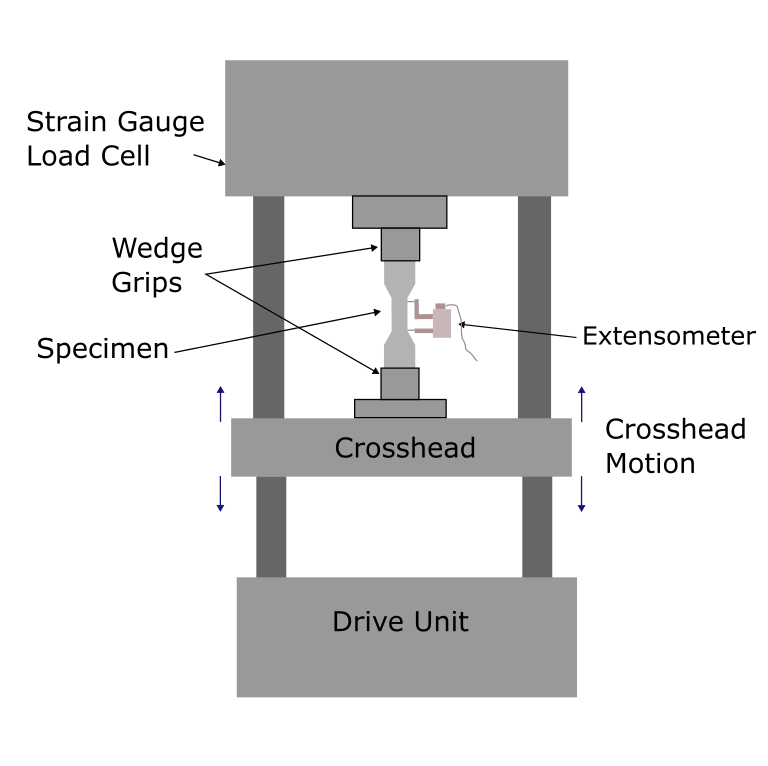
\includegraphics[width=\textwidth]{Images/chapter1/uniaxialtension.png}
        \caption{Low strain rate test with a standard tensile machine}
        \label{fig:subfiglow}
        \end{subfigure}
        \hfill
        \begin{subfigure}[b]{0.45\textwidth}
        \centering
        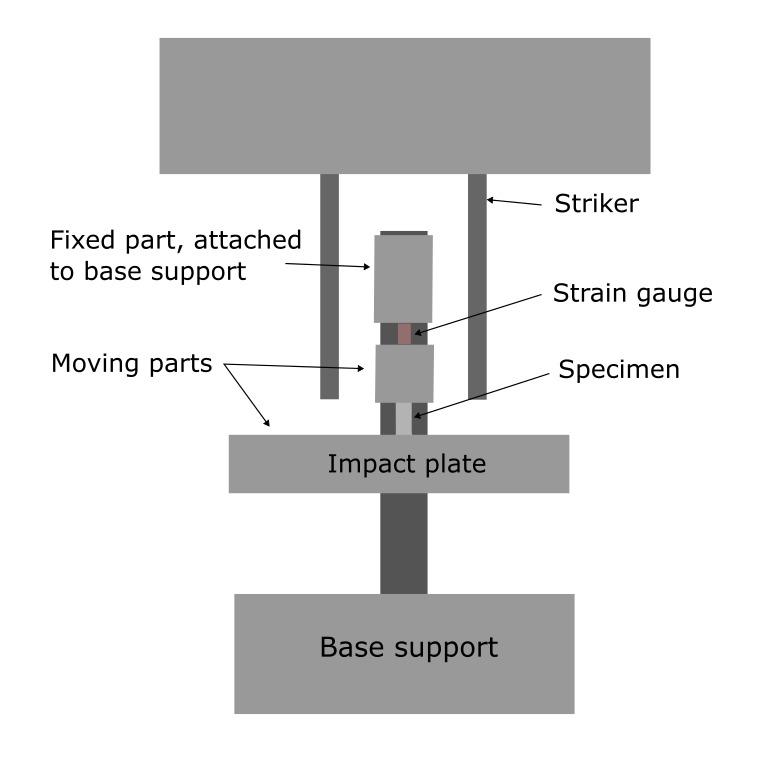
\includegraphics[width=\textwidth]{Images/chapter1/uniaxialintermediate.png}
        \caption{Intermediate strain rate test with a falling weight impact tester}
        \label{fig:subfiginter}
        \end{subfigure}
        \vspace{0.5cm}
        \begin{subfigure}[b]{0.7\textwidth}
        \centering
        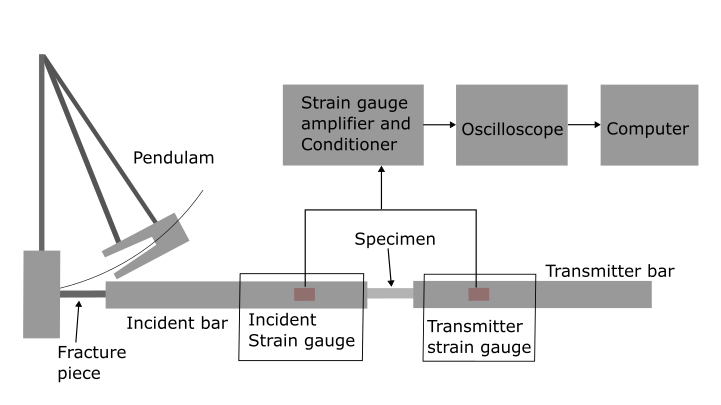
\includegraphics[width=\textwidth]{Images/chapter1/uniaxialhigh.png}
        \caption{High strain rate test with a split Hopkinson pressure bar in tension}
        \label{fig:subfighigh}
        \end{subfigure}  
        \hspace{0.3cm}

        \caption[Uniaxial tensile testing of ether-based polyurethane]{Uniaxial tensile testing: Diagram of three tensile testing of an ether-based polyurethane elastomer specimen done with three different experiment configurations for different strain rate analysis. Diagrams are based on the experiments of made by \citet{Kanyanta2010}.}
        \label{fig:uniaxialkan}
\end{figure}

For the low strain rate tensile tests ($< \SI[per-mode = symbol]{1}{\per \second}$), a standard Instron machine was utilized, as illustrated in Figure 
\ref{fig:subfiglow}. Intermediate strain rate tensile tests (between $\SI[per-mode = symbol]{1}{\per \second}$ and $\SI[per-mode = symbol]{100}{\per \second}$) 
were performed using a drop-weight tester (Fig. \ref{fig:subfiginter}). Load measurements were recorded with a calibrated strain gauge, 
with the zero position established at the striker and impact plate's initial contact point.
High strain rate tests ($>\SI[per-mode = symbol]{100}{\per \second}$) were conducted with a split Hopkinson pressure bar in tension, as shown in Figure \ref{fig:subfighigh}.
A swinging pendulum generated a tensile pulse, propagating along the bar into the specimen. Utilizing 
the transmitted and reflected strain signals and using the classical Kolsky analysis the specimen stress
\begin{align}
        \sigma(t) = E\frac{A_b}{A_s}\epsilon_t(t) \, ,
\end{align}
and the strain
\begin{align}
        \epsilon(t) = \frac{-2C_b}{l_s} \int_{0}^{t} \epsilon_r(t) dt \, ,
\end{align}

were calculated. Here, $A_b$ is bar's cross-sectional area, $A_s$ the specimen's cross-sectional area,
$\epsilon_t$ refers to the transmitted strain signal, $\epsilon_r$ is the reflected strain signal,
$l_s$ is the specimen gauge length, and $C_b$ is the wave speed through the bar.
Low strain rate tests were conducted under dry-room temperature, wet-room temperature, and wet at $\SI{37}{\degreeCelsius}$. 
Intermediate and high strain rate tests were performed exclusively under dry-room temperature conditions.\\

Test results demonstrated that ether-based polyurethane elastomer specimens were highly sensitive to 
temperature and humidity, as the material softened with increased levels of these factors. Young's 
modulus values for dry-room temperature setup $\SI{7.4}{\mega \pascal}$, decreasing to $\SI{5.3}{\mega \pascal}$ 
and $\SI{4.7}{\mega \pascal}$ for the wet-room temperature and wet conditions, respectively.
Moreover, the polyurethane exhibit varying Young's modulus values under dry-room temperature, depending 
on the elastomer's composition, with values ranging from $\SI{3.6}{\mega \pascal}$ to $\SI{14.8}{\mega \pascal}$.

The material displayed minimal strain rate dependency at low strain rates, but exhibited moderate 
strain rate sensitivity at intermediate and high strain rates, where the Young's modulus ranged between 
$\SI{8}{\mega \pascal}$ and $\SI{12}{\mega \pascal}$. However, for strains below $\SI{20}{\percent}$, the 
outcomes showed repeatability across all strain rates tests. 

For strain rates found in arteries around $<\SI[per-mode = symbol]{2}{\per \second}$, the variation of the
Young's modulus was insignificant and this could be assumed to be constant. This study demonstrated 
that it is important to measure the properties of the elastomer under similar condition to the
intended application, as properties varies under different conditions.

\subsubsection*{Uniaxial Compression Testing}
Compression tests are also widely utilized to determine the stress-strain response and 
usually involve placing the specimen in between two plates and compressing the material (Fig. \ref{fig:compressiondiag}).
The stress-strain response derived from this kind of testing serves in determining the deformation 
characteristics of the material including the fatigue and fracture resistance. 
Uniaxial compression tests may be affected by the interface friction between the specimen and 
the loading plates, leading to a nonhomogeneous deformation state, e.g., barrelling \cite{Bergström2015}.\\

\begin{figure}%
        \centering
       \quad
       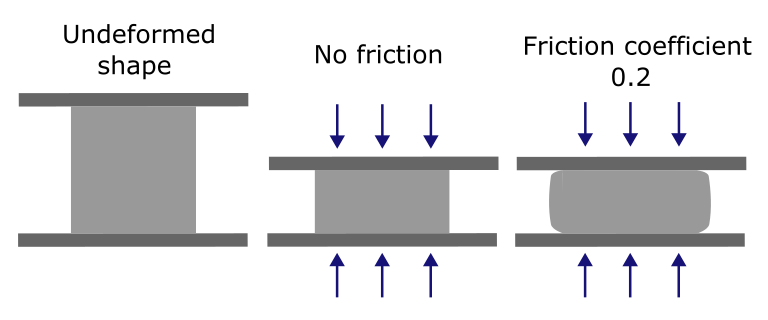
\includegraphics[width=10cm]{Images/chapter1/compressiondiag.png}%
       \caption[Uniaxial compression testing setup]{Uniaxial compression testing: Diagram of typical compression setup and influence of interface friction on the deformed specimen shape. Illustration is based on the "Mechanics of Solid Polymers" by \citet{Bergström2015}.}%
       \label{fig:compressiondiag}%
\end{figure}

\citet{Drass2018} conducted a uniaxial compression test, showing that the lubrication was 
crucial for an homogenous stress and strain distribution. The specimen tested was made from Transparent Structural 
Silicone Adhesive (TSSA), a rubber-like material commonly used in laminated connections within glass structures.
In this study homogeneous and inhomogeneous experiments were performed, as the goal was to determine an 
experimental setup, which ensured an homogeneous stress and strain distributions for the identification of material parameters \cite{Drass2018}.

The specimen was compressed with perfect slippage, where the plates and the specimen were lubricated 
before testing to ensure a frictionless support. A constant speed of $v_{UC}=\SI[per-mode = symbol]{0.174}{\milli \m\per \minute}$
was used for this test with a saBesto HHS 5000 machine. The compression test were consucted until a strain $\epsilon=\SI{0.6}{}$ 
was reached, as the standard deviation for large compression strain ($\epsilon > \SI{0.5}{}$) was too large.
The test presented challenges in maintaining the lubrication throughout the test, as it tended to be 
pressed out between the test specimen and the pressure plates, resulting in a increased friction. 

The results of this experiment were processed to identify hyperelastic material parameters using standard 
fitting routines and inverse methods. The test suggested that only stress-strain response up to a strain value of 
$\epsilon=\SI{0.5}{}$ should be considered for the indentification of the TSSA material parameters, as 
the friction's impact can be neglected for smaller strains.\\

In comparison, for a biomaterials, e.g., human soft tissues, a compressive testing of cartilage was conducted by \citet{Griffin2016}. 
This study aimed to provide a protocol were compressive and tensile properties of human soft tissues can be evaluated 
and characterized with minimal destruction. By understanding these material's properties and calculating the Young's 
elastic modulus, it would be possible to obtain a benchmark for creating suitable tissue-engineered substitutes \cite{Griffin2016}. 

The mechanical response of cartilage is highly dependant to the fluid's flow through the tissue. The methods for compression 
testing can vary with confined or unconfined specimen, and the most prevalent, indentantion (Fig. \ref{fig:compressiontypes}).
In the unconfined compression the cartilage is pressured using a non-porous plate onto a non-porous chamber, 
leading to a predominatly radial fluid flow. For the confined compression the sample was placed in a sealed, 
fluid-filled impermeable chamber and loaded with a porous plate, making the fluid flow restricted to a vertical direction.
Finally, the indentation testing employed a smaller indenter applied to the sample's surface perpendicularly, ensuring 
uniaxial compression and minimizing shear loading. All test were conducted in a 
hydrated environment and the cartilage was submerged in phosphate-buffered saline before and during the test to maintain 
the hydration. With the latest compression testing type it was possible to identify elastic and viscoleastic properties 
of the sample \cite{Griffin2016}.

\begin{figure}%
        \centering
       \quad
       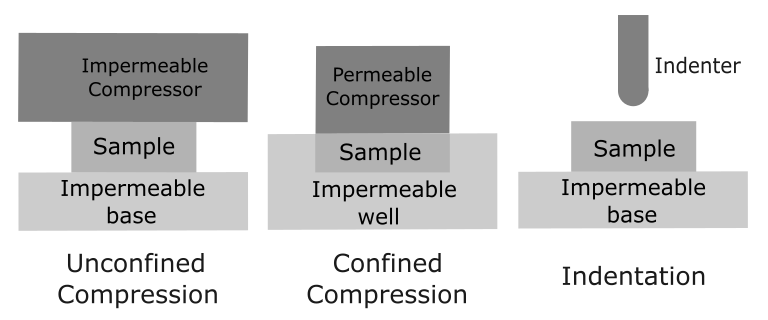
\includegraphics[width=10cm]{Images/chapter1/compressiontypes.png}%
       \caption[Uniaxial compression testing methodologies]{Uniaxial compression testing: Illustration of different compression methodologies for a cartilage specimen. Unconfined compression, confined compression and Indentation. Diagrams are based on the methodologies showed by \citet{Griffin2016}.}%
       \label{fig:compressiontypes}%
\end{figure}

%------------------------------------------------------------------------
\subsubsection*{Indentation}
Indentation testing, including micro and nanoindentation, is a popular method for characterizing 
the mechanical properties of soft materials \cite{Wu2016}. One of the main advantages of 
indentation testing is that it requires minimal sample preparation and it is often a 
nondestructive technique, which allows the preservation of the geometry and tissue's architecture \cite{Shi2019}.
Furthermore, indentation is useful where more traditional testing techniques such as 
uniaxial or biaxial testing, are not possible to employ, 
and can also be utilized to evaluate nonlinear properties, e.g., viscoplastic responses\cite{Bergström2015}.\\

Despite these advantages, there are challenges when using indentation to 
characterize soft materials. First, a stress-strain response is difficult to
obtain due to the complex boundary conditions, which introduces an inverse problem 
for the identification of material parameters \cite{Shi2019}. Second, many of the current 
indentation configurations assume material isotropy, which may not be the case for biomaterials \cite{Feng2017}.
In addition, determining the mechanical properties of soft materials locally or at small scales is still difficult to achieve \cite{Zhang2014}.


The usual indentation testing setup is shown in Figure \ref{fig:Nanoindentation}, in this case a 
system applies a certain force to an attached indenter rod where and specific 
indenter tip. After the indenter tip goes to a determined displacement, 
it is possible to obtain a load-displacement curve.
The deformation can be measured through an capacitance gauge or also optically, via laser measurements \cite{Bergström2015}.\\

\begin{figure}[th]
        \centering
        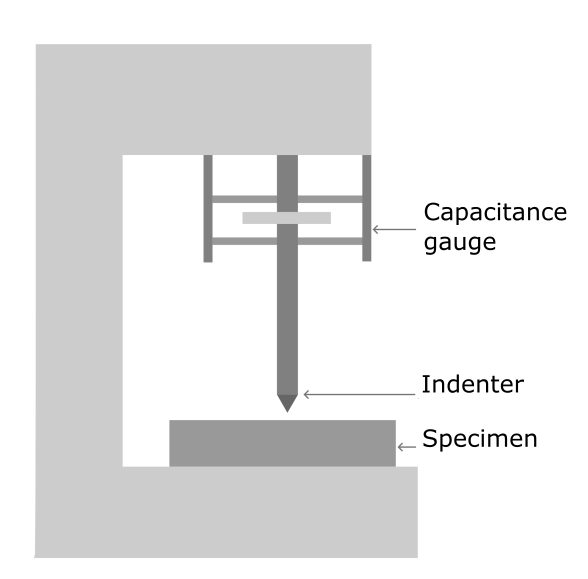
\includegraphics[width=7cm]{Images/nanoindentationbigletter}
        \caption[Nanoindentation experiment diagram]{Nanoindentation experiment setup diagram with an indenter tip attached to a rod and a polymer as specimen. Diagram is based on the "Mechanics of Solid Polymers" by Bergström \cite{Bergström2015}.}
        \label{fig:Nanoindentation}
\end{figure}

In a study made by \citet{Zhang2014} an investigation of spherical indentation on hyperelastic 
soft materials was conducted. The material utilized in the experiments was polydimethylsiloxane (PDMS),
with was prepared and cured in a cylindrical mold and cured at $\SI{60}{\degreeCelsius}$ for eight hours. 
The ElectroForce 3100 was used to measuring the mechanical properties of PDMS for tensile and 
indentation tests. Tensile tests were performed to identify the initial shear modulus and 
locking stretch and their results compared with the indentation tests \cite{Zhang2014}. 
For the indentation tests an spherical indenter with a $\SI{3}{\milli \m}$ radius with a similar configuration 
shown in Figure \ref{fig:Nanoindentation} was used. The measurements were done under room temperature and 
a humidity of $\SI{50}{\percent}$ with a loading rate of $\SI[per-mode = symbol]{2}{\milli \m\per \second}$ and 
a indentation depth of $\SI{3}{\milli \m}$. Six measurements were carried out at different 
locations on the specimen, generating an indentation load-displacement curves. 
Moreover, the initial shear modulus was determined using fitted results of the load-depth curves to 
the Hertzian and hyperelastic solution developed in the study.

The results exhibited that the determination of the initial shear modulus was possible but a 
certain depth depence coudl be observed. However, a locking stretch could not be analyze due to the 
sensitivity of these parameters to experimental data noise \cite{Zhang2014}.\\

For an application with biological tissues \citet{Carter2001} performed indentation experiments on 
human and porcine organs for its application in realistic computer-based simulators 
for minimal access surgery (MAS) training. 
This study investigated the stress-strain data pig spleen and liver for \textit{ex vivo} experiments, 
along with human liver for \textit{in vivo} experiments from volunteers patients undergoing a minor 
surgery. For the \textit{ex vivo} experiment a static indentation setup was used as shown in Figure 
\ref{fig:carter1}, where the specimens were placed on a flat surface. A force was applied 
manually with a winding mechanism at constant rate of $\SI[per-mode = symbol]{1}{\milli \m\per \second}$ 
with a rounded indenter with a diameter of $\SI{4.5}{\milli \m}$. Ten measurements were 
carried out on each tissue sample and the load-displacement measurements were 
gathered with a computerized system with a sampling rate of $\SI{15}{\hertz}$.\\

\begin{figure}
        \centering
        \begin{subfigure}[b]{0.45\textwidth}
        \centering
        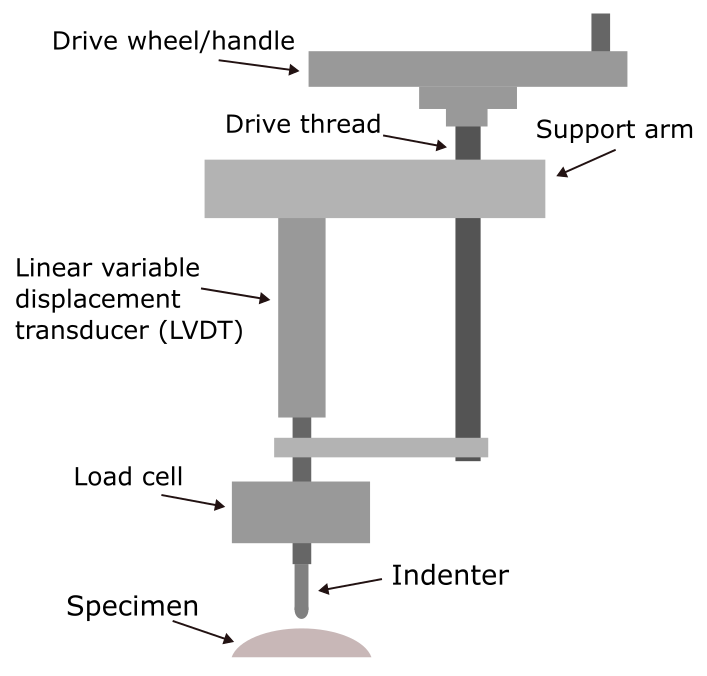
\includegraphics[width=\textwidth]{Images/chapter1/indentation1carter.png}
        \caption{Static indentation configuration used for \textit{ex vivo} indentations tests. Indenter advances against the tissue by rotating the wheel}
        \label{fig:carter1}
        \end{subfigure}
        \hfill
        \begin{subfigure}[b]{0.45\textwidth}
        \centering
        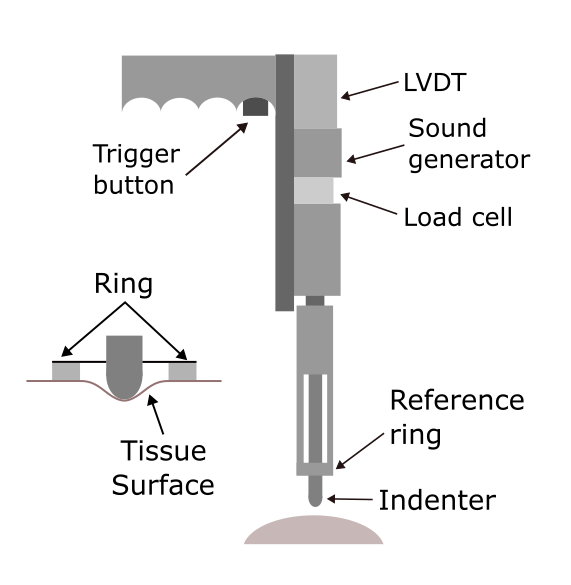
\includegraphics[width=\textwidth]{Images/chapter1/indentation2carter.png}
        \caption{Mobile indentation configuration with outer ring case attached for stabilization of the indentation test.}
        \label{fig:carter2}
        \end{subfigure}
        \hspace{0.3cm}
        \caption[Indentation setup of synthetic and biological tissues]{Indentation testing: Diagram of static and mobile indentation tests, indenters were attached to a load cell, which was connected to a displacement transducer. Diagrams are based on the study of made by \citet{Carter2001}.}
        \label{fig:indentationcarter}
\end{figure}

The \textit{in vivo} experiments were carried out using a hand-held compliance probe. To achieve 
an overall consistency of the measurements the same surgeon performed the experiments. 
In addition to maintain consistent indentation depth of $\SI{5}{\milli \m}$ the indenter was 
surrounded with a reference ring to provide stability in the measurements (Fig. \ref{fig:carter2}). The force 
exerted by the weight of the ring was around $\SI{0.5}{\newton}$, while the friction force 
between the ring and the surface tissue was below $\SI{0.05}{\newton}$, making it a negligible 
effect. The probe was positioned on the tissue and when the desired indentation depth was 
indicated with an audible signal. The indentation rate for this configuration ranged 
from $\SI[per-mode = symbol]{3}{\milli \m\per \second}$ to $\SI[per-mode = symbol]{4}{\milli \m\per \second}$ and 
six measurements were carried out on each patient.

The results were analyzed using MATLAB and showed highly nonlinear stress-strain behavior and large variances. 
For the reduction of these variances due to the inhomogeneity of the materials and changes over time, 
the average of the repeated measured was calculated. The measured elastic moduli of pig 
spleen and liver was $\SI{0.11}{\mega \pascal}$ and $\SI{4}{\mega \pascal}$ respectively, and 
for the human liver about $\SI{0.27}{\mega \pascal}$ was measured. However, a 
diseased liver showed a higher elastic modulus of $\SI{0.74}{\mega \pascal}$ \cite{Carter2001}.
%-------------------------------------------------------------------------------------------------
\subsubsection*{Aspiration Experiment}

Tissue aspiration experiments was a method introduced by \citet{Kauer2002} for determining 
the material parameters of biological soft tissues \textit{in vivo}.
In this study the method was validated with a synthetic material, Silgel, a very 
soft gel-like material with similar properties to biological soft tissues. 
This material was ideal to use it for the validation of the 
aspiration method before applying it to human tissues \cite{Kauer2002}.

The biological sof tissue used in this paper was human uterus. This tissue was selected 
because it possesses a complex, multilayered structure with anisotropic properties. 
Moreover, hysterectomy (removal of the uterus) is common surgical procedure, which 
provides a good chance to perform measurements before and after the removal of the organ.\\

This method introduced an aspiration tube which is put against the 
soft tissue, generating a vacuum a causing the deformation of the tissue (Fig. \ref{fig:aspiration} ). 
An advantageous feature of this experimental technique is that 
it can be perfomed \textit{in vivo} and \textit{ex vivo}.
With the help of a mirror placed next to aspiration hole, the reflection 
of the side-view of the tissue can be captured with a video camera.
This camera captures the images of the iluminated surface of the material and the 
aspiration pressure is captured through a sensor. Through this process the captured 
profile of the tissue is obtained and this can be used to characterize the deformation 
and analyze the viscoelastic properties of the soft tissue \cite{Kauer2002}.

\begin{figure}[th]
        \centering
        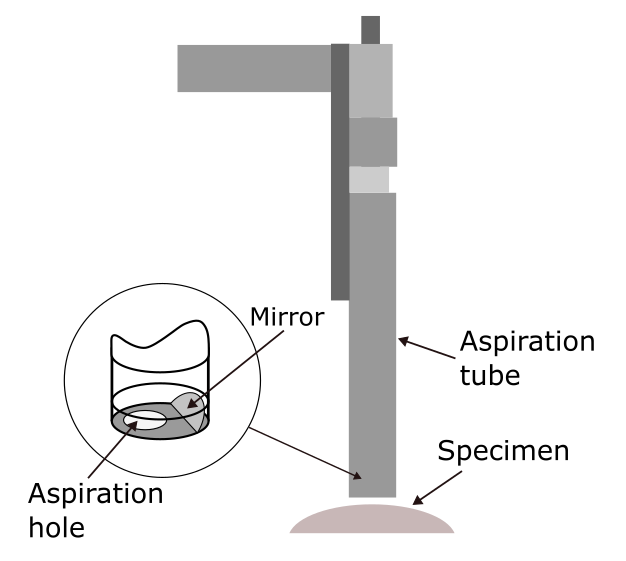
\includegraphics[width=7cm]{Images/chapter1/aspirationkauer.png}
        \caption[Aspiration experiment]{Aspiration experiment setup: Diagram showing aspiration tissue vertically positioned to the target tissue, inside of the tube a mirror reflects the side view of the tissue to the video camera on top. Diagram based on the research of \citet{Kauer2002}.}
        \label{fig:aspiration}
\end{figure}

The main benefits in comparison to more traditional experimental techniques are, 
the well-defined mechanical boundary conditions during the experiment are executed, 
large deformation experiments can be assessed, and the viscoelastic
properties of the tissue can be analyzed for real surgical procedures due to 
the time dependent resolution of the deformation.

The results from these experiments corroborates that the development of experimental designs for
biological soft tissues and its application in real-world scenarios is essential to understand 
their mechanical behavior and make advance in medical research.

%---------------------------------------------------------------------------------
\subsection{Material Modeling of Soft Materials}
\label{subsection:materialmodeling} 

Material models, such as linear elasticity and hyperelasticity play a crucial role for the characterization 
of material properties, as these describe a relationship that represents how a material behaves, e.g, 
the stress response for an applied strain, or the heat transfer for a defined temperature gradient.
For the case of soft materials, hyperelastic models are usually 
useful candidates, as these models can often predict the behavior of complex materials under certain limitations.
Moreover, hyperelastic models can be used as a foundation for more advance models like 
viscoelastic and viscoplastic models \cite{Bergström2015}. 

Hyperelastic models are useful due to their ease of use and calibration, accessibility in major commercial FE softwares, 
and computational efficiency. However, these models possess some limitations, such as being 
accurate for monotonic loading, and not capturing rate effects, i.e., viscoelasticity, or 
hysteresis during cyclic loading \cite{Bergström2015}.

In this subsection, linear elasticity and hyperelasticity constitutive models will be presented 
based on the overview made by \citet{Bergström2015}, followed by examples from the research 
papers from the Subsection \ref{subsection:experimentalcharacterization} to confirm the relevance of these 
models for medical research.

\subsubsection*{Linear Elasticity}
This model is the most basic approach to represent the small strain of the mechanical behavior 
of solid polymers, with isotropic elasticity being its most elementary form \cite{Bergström2015}.
In isotropic elasticity, stress is proportional to the applied strain and independent of the material's 
orientation. Hooke's law is frequently the constitutive equation for an elastic material, and one form 
\begin{align}
        \epsilon_{ij} &= \frac{1 + \nu}{E} \sigma_{ij} - \frac{\nu}{E} \sigma_{kk} \delta_{ij} \, ,
        \label{eq:linearelasberg}
\end{align}  
was presented by \citet{Bergström2015} to define a strain-stress relationship, where the indices $i$ and $j$ take the values of 
$\SI{1}{}$, $\SI{2}{}$, and $\SI{3}{}$, $\epsilon_{ij}$ and $\sigma_{ij}$ are the strain and stress tensors, and
\begin{align}
        \delta_{ij} = \begin{cases} 
                        1, & \text{if } i=j, \\
                        0, & \text{otherwise},
                      \end{cases}
\label{eq:kronecker}
\end{align}
represents the Kronecker delta function. Similarly, the stress 
\begin{align}
        \sigma_{ij} = 2\mu\epsilon_{ij} + \lambda\epsilon_{kk}\delta_{ij} \, ,
        \label{eq:sigmalinearberg}
\end{align}
can be determined in terms of the strain using Hooke's Law. Key parameters in Equations \ref{eq:linearelasberg}
and \ref{eq:sigmalinearberg} include the Young's Modulus $E$, Poisson's ratio $\nu$, the shear modulus $\mu$, 
and the Lame's constant $\lambda$. 
The linear elastic constitutive theory can be formulated with the identification of two material parameters,
which can be determined through experimental data. After identifying these two parameters, it is possible to  
calculate any other constants. A typical experimental method to identify and calibrate a pair of parameters is the uniaxial tension 
test, where the stress-strain response identifies $E$ and $\nu$.
A significant drawback of using a linear elastic model to predict the mechanical behavior of soft polymers is 
that these materials exhibit linear behavior only within small strains and a limited range of strain-rates and 
temperatures \cite{Bergström2015}. 

\subsubsection*{Anisotropic Elasticity}
Anisotropic elasticity is an extension of linear elasticity theory that considers the anisotropic 
behavior of the material, as is usually the case for biopolymers. The strain $\epsilon_{ij}$ and stress $\sigma_{ij}$ 
\begin{align}
        \epsilon_{ij} &= S_{ijkl} \sigma_{kl}, \label{eq:strainanisotropic}\\
        \sigma_{ij} &= C_{ijkl} \epsilon_{kl}, \label{eq:stressanisotropic}
\end{align}
can be written using Hooke's Law for an anisotropic material. These equations 
show that the stress and strain tensor are linearly dependent on each other by a linear stiffness $C_{ijkl}$ 
or compliance tensor $S_{ijkl}$. The stiffness and compliance tensors possess $\SI{81}{}$ components and 
since the stress and strain tensors are symmetrical, the independent components of $S$ and $C$ can be then reduced 
to $\SI{36}{}$ components. Depending on the degree of anisotropy, these matrices can be further simplified. 

\subsubsection*{Hyperelasticity}
Hyperelastic models are an extension of linear elasticity that accounts for nonlinearity 
and large strain predictions. These models have been widely developed over the years and 
are available in various FE softwares. Hyperelastic models are very important in modeling 
soft tissues, as they can be sometimes connected to the micromechanisms driving the 
deformation behavior of the material \cite{Bergström2015}. Common hyperelastic models include the 
Neo-Hookean, Mooney-Rivlin and Ogden models.\\

\textbf{Neo-Hookean Model}\\

The Neo-Hookean (NH) model consists of a simple hyperelastic model based on the shear 
modulus $\mu$ and the bulk modulus $\kappa$. This model can be used for compressible 
and incompressible deformations, with the compressible version often being more 
practical for finite element simulations. The NH model is primarily used for 
solid, rubber-like materials characterized by an almost incompressible behavior. 
Because of this characteristic, the actual value has a minimal effect on the response 
of the observed material \cite{Bergström2015}.

The NH model is like other hyperelastic models, specified by its Helmholtz free energy per unit 
reference volume
\begin{align}
        \psi(I_1^*,J) = \frac{\mu}{2}(I_1^* - 3) + \frac{\kappa}{2}(J - 1)^2 \, ,
        \label{eq:helmholtzNH}
\end{align}
where $I_1^*$ is the distortional first invariant, and $J$ the Jacobian of the deformation gradient \cite{Youssef2022}.
This equation is inadequate for the accurate description of large-strain nonlinear responses. 
In addition, this equation is not dependent on the second invariant $I_2^*$, which limits the 
stress prediction for biaxial loading.

The Cauchy stress for compressible NH model can be expressed as \cite{Youssef2022}
\begin{align}
        \sigma = \frac{\mu}{J}\text{dev}[\boldsymbol{b}^*] + \kappa(J-1)\boldsymbol{I} \, ,
        \label{eq:cauchystressNHcomp}
\end{align}
where $\boldsymbol{b}^*$ left Cauchy-Green strain tensor, and $\boldsymbol{I}$ is the identity matrix. 
The Cauchy stress expressions for uniaxial, planar and biaxial deformations for incompressible NH models are
\begin{align}
        \sigma_{\text{uniax}} &= \mu(\lambda^2 - 1/\lambda), \label{eq:uniaxNH} \\
        \sigma_{\text{planar}} &= \mu(\lambda^2 - 1/\lambda^2), \label{eq:planarNH} \\
        \sigma_{\text{biaxial}} &= \mu(\lambda^2 - 1/\lambda^4), \label{eq:biaxialNH}
\end{align}
respectively. In these equations, $\lambda$ represents the stretches of the deformation \cite{Youssef2022}.
An alternative formulation of the NH model, where the stress is not divided into deviatoric and volumetric 
parts, is given by
\begin{align}
        \sigma = \frac{\mu}{J}(\boldsymbol{b}-\boldsymbol{I}) + \kappa(J-1)\boldsymbol{I}. \label{eq:stressNHalt}
\end{align}
The predictions from the standard NH model (Eq. \ref{eq:cauchystressNHcomp}) and this alternative formulation 
(Eq. \ref{eq:stressNHalt}) becomes different with the decrease in the bulk modulus.
The main advantage NH model lies in its simplicity; with the shear modulus known, the response of almost any loading 
mode can be determined in a robust, and computationally efficient way. However, the limitations of the model lies 
in capturing large-strains or when the loading is primarily biaxial \cite{Bergström2015}.\\

The Neo-Hookean model has been employed in various research papers to characterize soft tissue behavior. 
For instance, in a study from Kanyanta and Ivankovic (2010) used and compared different hyperelastic models to characterize different loading 
of an ether-based polyurethane (see Subsection \ref{subsection:experimentalcharacterization}). Here the elastomer was assumed to 
be an isotropic, incompressible material for the description of the behavior of polyurethane \cite{Kanyanta2010}.

Furthermore, Chai et al. (2013) utilized the Neo-Hookean model to calculate the Young's modulus of human carotid plaques
assuming an isotropic, incompressible model. This knowledge contributes to the identification of local biomechanical properties 
of atherosclerotic plaque tissue for more reliable rupture risk prediction \cite{Chai2013}.

In another study made by Shi et al. (2019), a compressible NH model was used to describe the ground substance of the 
fiber network of the cervical stroma. Using this model it was possible to identify the $\mu$ and $\lambda$ and then calculate the Young's modulus and 
Poisson's ratio \cite{Shi2019}.\\

\textbf{Mooney-Rivlin}\\

The Mooney-Rivlin (MR) mode is a model that builds upon the NH model by incorporating a linear dependence on the 
second invariant $I_2^*$ in the Helmholtz free energy per unit reference volume equation 
\begin{align}
        \psi(C_{10}, C_{01}, \kappa) = C_{10}(I_1^* - 3) + C_{01}(I_2^* - 3) + \frac{\kappa}{2}(J-1)^2 \, ,
        \label{eq:helmholtzMR}
\end{align}
where $C_{10}$, $C_{01}$, $\kappa$ are the necessary material parameters for the compressible MR model \cite{Bergström2015}.
These parameters are defined based on the experimental data and for small strains, the shear modulus can be represented as \cite{Youssef2022}
\begin{align}
        \mu = C_{10} + C_{01} \, .
        \label{eq:constantsMR}
\end{align}
The Cauchy stress for the MR model can be expressed as 
\begin{align}
        \sigma = \frac{2}{J}(C_{10} + C_{01}I_1^*)\boldsymbol{b}^* - \frac{2C_{01}}{J}(\boldsymbol{b}^*)^2 + [\kappa(J-1) - \frac{2I_1^* C_{10}}{3J} - \frac{4I_2^* C_{01}}{3J}]\boldsymbol{I} \, .
        \label{eq:cauchystressMR}
\end{align}
For the incompressible version of the MR model, the Cauchy stresses in uniaxial, planar and equibiaxial deformations are 
\begin{align}
        \sigma_{\text{uniax}} &= 2(\lambda^2 - 1/\lambda)[C_{10} + C_{01}/\lambda] \, , \label{eq:uniaxMR} \\
        \sigma_{\text{planar}} &= 2(\lambda^2 - 1/\lambda^2)[C_{10} + C_{01}] \, , \label{eq:planarMR} \\
        \sigma_{\text{biaxial}} &= 2C_{10}(\lambda^2 - 1/\lambda^4) + 2C_{01}(\lambda^4 - 1/\lambda^2) \, . \label{eq:biaxialMR}
\end{align}
The Mooney-Rivlin model often enhances the accuracy of the predictions of the Neo-Hookean model.
However, certain loading modes can cause instability in the case of a negative $C_{01}$ term \cite{Bergström2015}.\\

Research papers, which used the Mooney-Rivlin model are, e.g., Drass et al. (2018) utilized the MR 
model to describe the behavior of silicone and identify the hyperelastic parameters through inverse methods. This model 
showed adequate results for the fitting of four different experimental methods; uniaxial tension and compression test, 
biaxial tension, and shear pancake test \cite{Drass2018}.

Likewise, this model was appropriate to simulate the nonlinear properties of breast soft tissues' deformation 
during a leaning forward position and running movement. By identifying the breast material properties, the bra-breast contact mechanism 
could be analyzed \cite{Sun2019}.\\

\textbf{Yeoh Model}\\

The Yeoh model (YM) is another hyperelastic model that utilizes a Helmholtz free energy 
in a third-order polynomial in $I_1^*$ and independent of $I_2^*$. This allows the model to provide 
more accurate predictions than the NH model, while potentially avoiding the stability issues of the 
MR model \cite{Bergström2015}. The Helmholtz free energy per unit reference volume for a compressible YM can be written as
\begin{align}
        \psi(C_{10}, C_{20}, C_{30}, \kappa) = C_{10}(I_1^* - 3) + C_{20}(I_1^* - 3)^2 + C_{30}(I_1^* - 3)^3 + \frac{\kappa}{2}(J - 1)^2 \, ,
        \label{eq:helmholtzYM}
\end{align}
where $C_{10}$, $C_{20}$, $C_{30}$, and $\kappa$ are the material parameters to describe this model. The Cauchy stress 
for the YM can be derived as 
\begin{align}
        \sigma = \frac{2}{J}(C_{10} + 2C_{20}(I_1^* - 3) + 3C_{30}(I_1^* - 3)^2)\text{dev}[\boldsymbol{b}^*] + \kappa(J - 1)\boldsymbol{I}\, .
        \label{eq:cauchystressYM}
\end{align}
The independence from the $I_2^*$ term is the main motivation for the Yeoh model. Due to the difficulty of experimentally 
determining the dependence of this term with the Helmholtz free energy, the neglect of this term in the YM makes 
it easier to apply. Moreover, the hyperelastic model is Drucker stable, which is another factor that facilitates the use of this model \cite{Bergström2015}.
For the incompressible version of the Yeoh model, the Cauchy stresses in uniaxial, planar, and equibiaxial deformations can be written as
\begin{align}
        \sigma_{\text{uniax}} &= 2[C_{10} + 2C_{20}(I_1 - 3) + 3C_{30}(I_1 - 3)^2](\lambda^2 - 1/\lambda) \, , \label{eq:uniaxYM} \\
        \sigma_{\text{planar}} &= 2[C_{10} + 2C_{20}(I_1 - 3) + 3C_{30}(I_1 - 3)^2](\lambda^2 - 1/\lambda^2) \, , \label{eq:planarYM} \\
        \sigma_{\text{biax}} &= 2[C_{10} + 2C_{20}(I_1 - 3) + 3C_{30}(I_1 - 3)^2](\lambda^2 - 1/\lambda^4) \, . \label{eq:biaxyM}
\end{align}
The Yeoh model has been proven to improve the prediction of the Neo-Hookean model in various loading modes, specially in large strain scenarios.
Bergström also mentions, that for the identification of the material parameters $C_{10}$ should be positive and $C_{20}$, and $C_{30}$ 
can be calculated as
\begin{align}
        C_{20} \approx -0.01C_{10} \,, \\
        C_{30} \approx -0.01C_{20} \, .
\end{align}

In the research of Kayanta and Ivankovic (2010), several constitutive models were compared for the description 
of polyurethane under different loading. The results of the Yeoh model showed the best fit to the variety of experimental data, however, 
the Neo-Hookean model showed to be adequate with small strain deformations \cite{Kanyanta2010}.
Additionally, Łagan et al. (2017) used the Yeoh model to analyze the accuracy of model fitting 
to the experimental data and estimate the mechanical properties of swine skin tissue in the abdominal region under uniaxial testing \cite{Lagan2017}.\\

       
\textbf{Ogden Model}\\

The Ogden model (OM) is a highly general hyperelastic model that is determined in terms of the applied principal stretches \cite{Bergström2015}.
Similar to the previous models, the Helmholtz free energy per volume can be written in various ways, 
\begin{align}
        \begin{split}
        \psi(\lambda_1^*, \lambda_2^*, \lambda_3^*) &= \sum_{k=1}^N \frac{2\mu_k}{\alpha_k^2}((\lambda_1^*)^{\alpha_k} + (\lambda_2^*)^{\alpha_k} + (\lambda_3^*)^{\alpha_k} - 3) \\
        &\quad+ \sum_{k=1}^N \frac{1}{D_k}(J - 1)^{2k} \,,
        \end{split}
        \label{eq:helmholtzOM}
\end{align}
being this equation, one of the most common for a compressible Ogden Model. Different from previously presented models, is that 
the volumetric response is not defined by the bulk modulus, but instead $D_k$ parameters. In this equation
$\mu_k$, $\alpha_k$, $\lambda_i^*$ are material parameters \cite{Youssef2022}. $\lambda_i^*$ are the deviatoric principal stretches defined as
\begin{align}
        \lambda_i^* = \frac{\lambda_i}{J^{1/3}} \,,
\end{align}
where, $\lambda_i$ are the principal stretches of the left Cauchy-Green tensor \cite{Ansys2010}. In addition, the initial bulk modulus 
can be defined from the incompressibility parameter $D_1$ as 
\begin{align}
        \kappa = \frac{2}{D_1} \,.
\end{align}
Equation \ref{eq:helmholtzOM} makes the Ogden model versatile, but can be complicated when selecting an appropriate 
set of material parameters that give stable predictions for the deformation states \cite{Bergström2015}. 
The principal $\sigma_i$ stresses can be expressed as
\begin{align}
        \sigma_i = \frac{2}{J}\sum_{k=1}^N \frac{\mu_k}{\alpha_k}((\lambda_i^*)^{\alpha_k} - \frac{1}{3}[(\lambda_1^*)^{\alpha_k} + (\lambda_2^*)^{\alpha_k} + (\lambda_3^*)^{\alpha_k}]) + \sum_{k=1}^N \frac{2k}{D_k}(J - 1)^{2k - 1} \,,
\end{align}
and the stresses for incompressible OM in uniaxial, planar and biaxial loading are given by
\begin{align}
        \sigma_{\text{uniax}} &= \sum_{k=1}^N \frac{2\mu_k}{\alpha_k}[\lambda^{\alpha_k} - (1/\sqrt{\lambda})^{\alpha_k}] \,,\\
        \sigma_{\text{planar}} &= \sum_{k=1}^N \frac{2\mu_k}{\alpha_k}[\lambda^{\alpha_k} - (1/\lambda)^{\alpha_k}] \,,\\
        \sigma_{\text{biax}} &= \sum_{k=1}^N \frac{2\mu_k}{\alpha_k}[\lambda^{\alpha_k} - (1/\lambda^2)^{\alpha_k}] \,.
\end{align}
The Ogden model turns equal to the Neo-Hookean model when $N = \SI{1}{}$ and $\alpha_2 = \SI{1}{}$.  
Moreover, the OM often shows a better prediction than the Neo-Hookean and Mooney-Rivlin models but is not accurate as the 
Yeoh model \cite{Bergström2015}.\\

Ahanchian et al. (2017) applied the first-order Ogden model to investigate the biomechanical behavior of 
human skin, particularly for the plantar heel pad tissue. This research led to a deeper understanding of 
the transfer of the load during walking when the foot impacts the floor,
and its implication in the design of shoe soles \cite{Ahanchian2017}.\\

In conclusion, the material modeling of soft materials is crucial for understanding their mechanical 
behavior and predicting their response to different loading conditions. Hyperelastic models, such as 
Neo-Hookean, Mooney-Rivlin, Yeoh and Ogden models, have been widely used to characterize synthetic and biomaterials 
due to their direct application and capacity to describe nonlinear behavior for small and large strains.
While these models have their respective advantages and limitations, they provide a basis level of understanding of 
complex material behavior and serve as a foundation for more advanced models. The selection of the models 
will depend on the specific intended use and the desired level of accuracy. 

%---------------------------------------------------------------------------------
\subsection{Inverse Finite Element Method for Parameter Identification}
\label{subsection:inverseFEMtheory}

The Inverse Finite Element Method (iFEM) has become a powerful technique and an increasingly 
popular approach for the identification of material parameters for both synthetic and biological materials \cite{Liu2009}. 
This method involves utilizing experimental data and numerical simulations to iteratively calibrate 
the material parameters until the computational model matches the experimental data. 
Furthermore, this approach aims to predict further experimental results with a validated computational model 
with an optimized set of material parameters, and extract and analyze more information about the material's behavior \cite{Kauer2002}.
In nonlinear cases, where the complexity of the problem increases, inverse FE methods are very useful \cite{Husain2004}.\\

The general iFEM process can be divided into the following steps:

\begin{enumerate}
        \item \textbf{Experimental data collection}: Experimental data of the observed material is gathered from the conducted mechanical tests, e.g., uniaxial tensile and compression testing, indentation, etc. This data, often given as a load-displacement, result is the basis for the identification of the parameters \cite{Seshaiyer2003}.
        \item \textbf{Finite element model development}: A finite element model is developed, which includes the definition of the geometry design, contact definition, boundary conditions and the selection of the appropriate material model \cite{Jamal2019}.
        \item \textbf{Initial parameter estimation}: Based on literature, experimental observations, or expert knowledge, initial estimates for the material parameters are chosen and input in the computational model \cite{Chawla2009}.
        \item \textbf{Optimization of the parameters}: With an optimization algorithm, the material parameters are iteratively calculated until the simulated response matches or reaches a good agreement with the experimental response. The Levenberg-Marquardt and the genetic algorithm are common algorithms employed in this step \cite{Kauer2002}.
        \item \textbf{Validation of the parameters}: The identified material parameters are validated by comparing the computational model predictions with the validation experimental data, which was not used in the optimization process \cite{Seshaiyer2003}.
\end{enumerate}

The main strengths of the iFEM is that this method allows the identification of parameters which are difficult to obtain 
through conventional methods and conserves the native geometry of the specimen. Furthermore, it is particularly advantageous for the 
solution and quantification of nonlinear problems with complex boundary conditions. A wide 
range of materials, including soft polymers and biological tissues can be analyzed, and this method allows the 
assumption of a homogeneous material, which helps in the description of local stresses and strain fields \cite{Seshaiyer2003}.\\

On the other hand, iFEM presents several limitations and challenges, this include the need for precise and dependable 
data, the potential for non-unique solutions in cases of poorly defined optimization, and the inability to find a 
unique set of parameters to describe all heterogeneous material regions. Also, iFEM with complex boundary conditions often demands
significant computational resources and requires a sturdy optimization algorithm \cite{Giudice2021}.\\

\subsubsection*{Synthetic Soft Materials}
Synthetic soft materials are commonly used to validate inverse parameter identification processes. 
They exhibit similar mechanical behavior to biomaterials, allowing researchers to validate the proposed 
inverse finite element approach before applying it to more challenging biomaterials, where \textit{in vivo} measurements are required.

For example, as mentioned in Subsection \ref{subsection:experimentalcharacterization} Silgel was used to validate an inverse
finite element method for characterizing the tissue of human uteri. The aspiration method was used for the experimental data collection, 
and the FE model of the deformation of the tissue on the aspirated area, required the contact 
between the tube and the tissue was treated as sticking. The strain energy function 
\begin{align}
        \bar{W} = (\sum_{k=1}^N \mu_i(J_1 - 3)^i) + \frac{1}{2}\kappa(J_3 - 1)^2 \,,
\end{align}
was selected for the explicit displacement-pressure finite element formulations \cite{Sussman1987}. 
This function depends on the reduced invariants $J_1$, $J_2$, $J_3$ of the right Cauchy-Green 
deformation tensor $\boldsymbol{C}$, and $\mu_i$ and $\kappa$ are the target material parameters. For $N = \SI{1}{}$ a nearly incompressible Neo-Hookean model 
is formulated, which was chosen for the case of Silgel. The Levenberg-Marquardt optimization method was selected for the optimization 
of three parameters: the shear modulus, and the bulk modulus. This method did not guarantee obtaining a global minimum, however after the selection of arbitrarily 
initial parameters, the objective function was minimized. With the set of parameters, the prediction of the tensile behavior was assessed with 
actual tensile tests. The prediction of the synthetic tissue demonstrated good prediction quality for these parameters \cite{Kauer2002}.

\subsubsection*{Biomaterials}

Ahanchian (2017) characterized the behavior of heel pad sub-layers utilizing the inverse finite element method.
%Experiment
With the aid of the ultrasound imaging and the indentation of the plantar heel pad tissue force-strain responses were recollected 
for the computational model. The contact between the indentation plate and the heel skin was set frictionless, and the first-order 
Ogden model was chosen for the description of the heel pad behavior. The Ogden strain energy function is
\begin{align}
        W &= \frac{\mu}{\alpha}((\lambda_1)^{\alpha} + (\lambda_2)^{\alpha} + (\lambda_3)^{\alpha} - 3) \,,
\end{align}
where $\lambda_i$ are the principal stretches, $\mu$ the shear modulus, and $\alpha$ the deviatoric exponent, being the last two
the hyperelastic material parameters. 
%FE
The indentation of the human heel was modeled to simulate the sub-layers of the human skin and the compression response of the material.
%Optimi
The RMS error 
\begin{align}
        \text{RMSE} &= \sqrt{\frac{\sum_{k=1}^N (F_s - F_e)^2}{n} }\,,
\end{align}
where, $F_s$ and $F_e$ are the simulated and experimental forces, respectively. The RMSE was the objective function to be minimized, 
and this process was done manually after each adjustment was input in the FE model. 
%validation
For the validation of  $\mu$ and $\alpha$ parameters, magnetic resonance imaging (MRI) was utilized.
A good agreement was achieved for the hyperelastic model between the simulations and the validation experiments. With this validated model 
a second stage was performed with a viscoelastic material model to improve the material model of heel skin sub-layers \cite{Ahanchian2017}.\\

In conclusion, integrating the iFEM with the experimental techniques and material models as presented in the previous sections, 
researchers can effectively identify material parameters for several synthetic and biological soft materials. 
This approach enables the development of accurate computational models that can be used to understand complex material behavior. 
%\subsection{Standard Verification and Validation for Computational Solid Mechanics (ASME)}
%\subsubsection*{VV40}
%---------------------------------------------------------------------------------

\section{Overview}
The thesis is organized into six chapters, providing an in-depth analysis of experimental models, computational models, 
parameter identification, optimization, and validation. 

%\textbf{Chapter 1} served as an introduction to the topic, setting the context and providing the motivation 
%for the work. It also presented an overview of the literature and the state of the art in the field.
\textbf{Chapter \ref{chapter:experimentalmodel}} details the experimental models used for the inverse finite element method. 
Indentation experiments were performed, and the experimental points are described. The chapter also outlines 
the main assumptions established for the development of the material model used in the FE model.

\textbf{Chapter \ref{chapter:computationalmodel}} focuses on the computational model, where the FE model is thoroughly described. 
Furthermore, the challenges encountered in the simulation process are also discussed, providing insights into 
the contact problem between the indenter and the material.

\textbf{Chapter 4} describes the inverse finite element method, explaining the process of material parameter identification. 
This chapter also describes the optimization methods explored, highlighting its importance in determining the best-fit 
material parameters for the experimental data.

\textbf{Chapter 5} presents the discussion of a proposed framework to develop a material model with iFEM approach 
and the results obtained from the iFEM, and the validation of the best material parameters are presented. 
This chapter assesses the accuracy of the identified parameters by comparing it with other validation experiments.
Finally, \textbf{Chapter 6} concludes the thesis by summarizing the main findings, discussing the implications of the results, 
and providing an outlook on future research directions and potential applications in further projects.
% Chapter 2

\chapter{Experimental Model} % Main chapter title
\label{Chapter3}

The design and selection of the experimental model is the first stage of this project.
This stage is mainly relevant to gather all the necessary data from the material, from which
the design parameters are searched.

This first experimental model had the purpose to serve as a comparator for the experimental 
model II (see section \ref{section:expmod2}). At the beginning of the project, the desired experimental 
model to be analyzed was the second experimental model, which was developed and designed by Yokohama National 
University (YNU). As this second experimental model was still undergoing some improvements and corrections, a similar 
experiment was designed which could served the same purpose.

The chosen experimental characterization for the inverse finite element method for 
 the identification of material parameters for this project was indentation.
The goal of these experiments was to observe the mechanical behavior of a soft material under 
compression using a rounded indenter. The aim was to determine the material behavior and 
observe the response under an indentation larger than the indenter radius. Additionally, 
by performing the indentation tests, the obtained 
data helped for a better understanding of the material's mechanical behavior for the chosen 
use cases and the determination of the main assumptions for the material modeling.
The main advantage of indentation is the noninvasive feature, which will mostly useful when 
identificating a part which should not be modified, e. g. an organ.

For both experimental setups the specimen, which was tested, was made from a two-component ultra-soft urethane resin.
This material, a synthetic soft material, was chosen because its material properities 
can simulate a biological tissue. %search reference
%here urethane resin avantages. and that it is expected that the material shows a 
\\ 

%----------------------------------------------------------------------------------

\section{Experimental Model I}
\label{section:expmod1}

%iii.	Analysis of different platforms
    
\subsection*{Description of the Experimental Setup}

The first indentation test configuration was done by adapting a tensile and compression 
testing machine, model LTS - 500 NB from MinebeaMitsumi.Inc (Fig. \ref{fig:firstexperiment}). This 
machine possess a maximum load capacity of \SI{500}{\newton}, and test speeds of
\SIlist[per-mode = symbol]{10;20;30;50;75;100}{\milli \metre \per \minute}. To achieve an 
indentation testing configuration, a pin was attached to the movable crosshead holding grip, 
as shown in Fig \ref{fig:500loadcell}.
The indenter had a rounded head made of stainless steel with a
radius of $r_p = \SI{3}{\milli \m}$ and a length of $l_p = \SI{11}{\milli \m}$.

\begin{figure}%
    \centering
   \subfloat[\centering Indentation test configuration with a \SI{500}{\newton} load cell \label{fig:500loadcell}]{{\includegraphics[width=6.5cm]{Images/Experiment/firstexperimentwithtext.png}}}%
   \qquad
   \subfloat[\centering Indentation test configuration with a \SI{10}{\newton} load cell \label{fig:10loadcell}]{{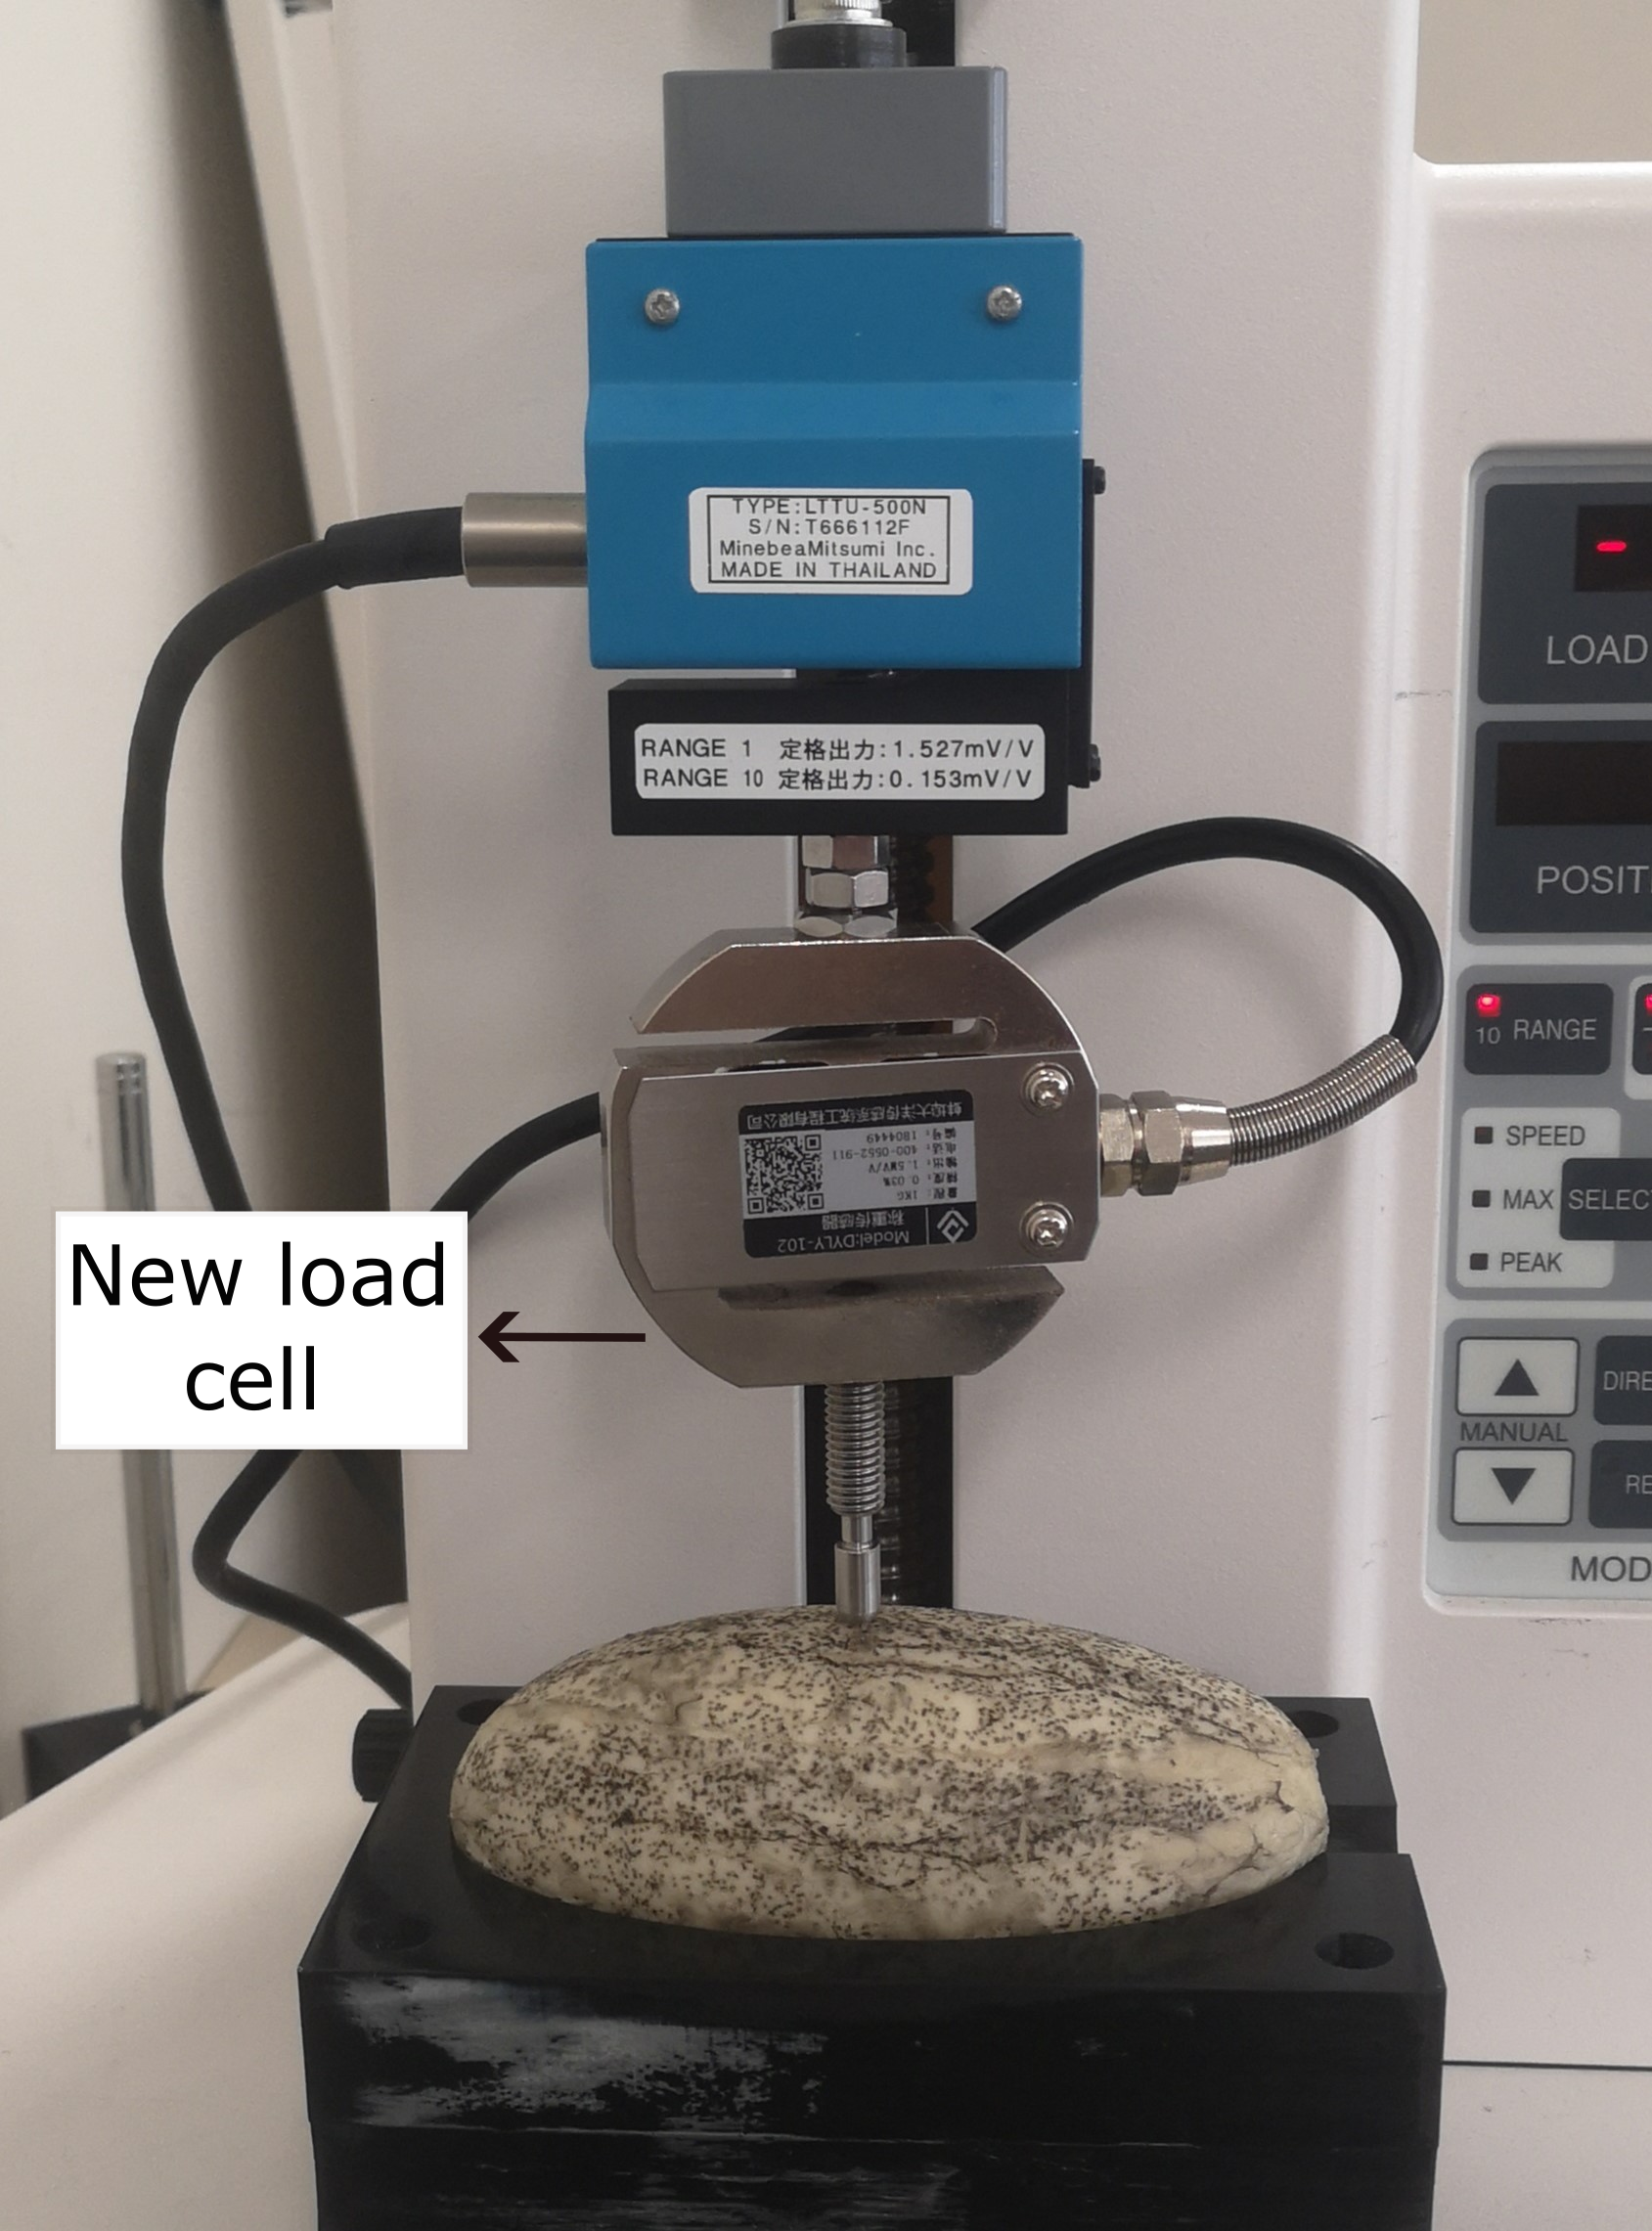
\includegraphics[width=6.5cm]{Images/Experiment/firstexpotherloadwithtext.png}}}%
   \caption{First experimental model: Tensile and compression machine with an indenter with a rounded head. Test Specimen made from ultra-soft polyurethane resin positioned on a fixed platform with a similar shape for constraint.}%
   \label{fig:firstexperiment}%
\end{figure}

The specimen possesses a ellipsoidal form with 
with a minor radius $r_1 = \SI{35}{\milli \m}$ and a major radius $r_2 = \SI{60}{\milli \m}$. 
This specimen geometry is supposed to simulate a kidney with an extracted tumor; therefore,
on the lower part of the specimen a half ellipsoid with a minor radius $r_{l1} = \SI{10}{\milli \m}$ 
and a major radius $r_{l2} = \SI{15}{\milli \m}$ was removed (Fig. \ref{fig:specimenhole}). 
The specimen was prepared by a YNU laboratory member, by 3D printing a mold with the wanted dimensions
 and a ellipsoidal shape, and filling it with liquid resin. 
 Additionally, it was left to cure for around \SI{30} hours. 
Then, the specimen was positioned on a platform fixed to the base, which suited 
the ellipsoidal geometry for properly constraint. 

\begin{figure}%
    \centering
   \subfloat[\centering Specimen dimensions bottom view \label{fig:specimenunder}]{{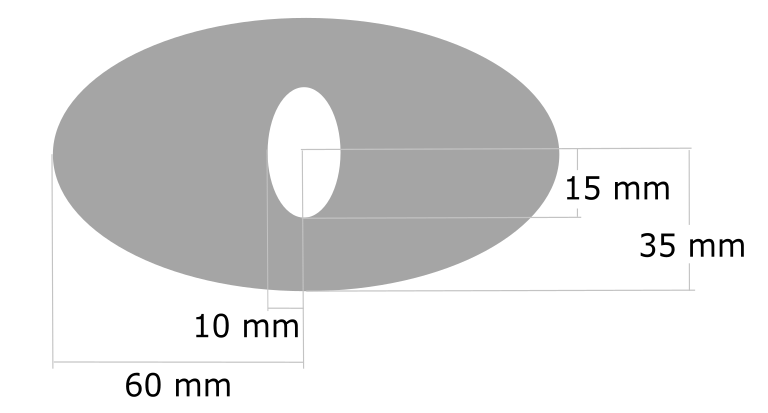
\includegraphics[width=6.5cm]{Images/Experiment/specimenhole.png}}}%
   \qquad
   \subfloat[\centering Specimen side view \label{fig:specimenside}]{{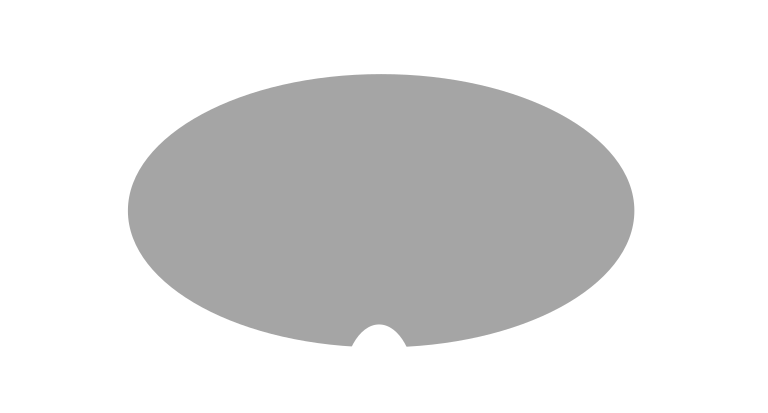
\includegraphics[width=6.5cm]{Images/Experiment/specimenholeside.png}}}%
   \caption{First experimental model: Specimen dimensions made from ultra-soft polyurethane resin for indentation test.}%
   \label{fig:specimenhole}%
\end{figure}

\subsection*{Procedure for Conducting the Experiment}
For the indentation test after placing the specimen on the platform,
the indenter was positioned slightly on the surface of the point of interest. 
The test was conducted with a room temperature of approximately \SI{22}{\degreeCelsius}
To perform the test the indenter was then lowered onto the surface of the specimen
at a velocity of \SI[per-mode = symbol]{10}{\milli \m\per \minute}.
The indentation depth was controlled by limiting the maximum depth, and the 
test stopped once the inserted depth was reached. The indenter returned to its 
original position after reaching the maximum depth with a rate of 
\SI[per-mode = symbol]{100}{\milli \m\per \minute}. Due to the material properties,
the specimen returned to its original shape.
The result of the indentation test was a load-displacement data,
which was recorded with a sampling rate of \SI{63}{\hertz} using a load 
cell of \SI{\pm 500}{\newton} and a encoder to measure the displacement.

The measurement accuracy according to the specification of the machine, has 
a relative reading error of \SI{1.0}{\percent}. The indentation test 
was repeated five times on the same sample to ensure and observe 
reliability and repeatability. Furthermore, the raw data collected from the test 
was processed and analyzed using Excel.

During the initial indentation test using the \SI{500}{\newton} load cell, 
the collected experimental data showed noise that could affect the accuracy 
and reliability of the results. The noise was likely caused by sensitivity 
of the lead cell. The ultra-soft polyurethane material showed force readings, which 
were near the lower limit of the load cell's range, which adding any other external factors, 
results in noisy measurements. To address this issue, a load cell of \SI{10}{\newton}
was installed (Fig. \ref{fig:10loadcell}). This change improved the quality of 
the measurements and reduced the noise in the data. The change to the load cell had some 
implication to the experimental setup, such as removing the holding grip, and designing 
a part which could connect the indenter with the new load cell. In addition to changing 
the load cell, a simple filtering method was used to improve the experimental data. After 
applying the filter, the noise in the data was reduced, resulting in more smoother 
force reaction readings. 

Overall, the applications of the combinations helped to improved the quality and acuracy 
of the data and gave important information about possible measurement errors to 
take into consideration for of the experimental model 
designed by YNU. At last, The filtered data was used for subsequent analysis and 
interpretation for the inverse finite element method approach for the material parameter 
identification.



% The approximated polynomial curve was used as a reference for the material modeling.

%test specimen is loaded at a quasi-static rate

% The measured force reation \(F_1\) data showed a very small number, so the 
% first 50 N load cell displayed a lot of noise in the measurements. 
% Therefore, the load cell was change to 10N to reduce this interference. 
%The 10 N load cell displayed the force-displacement curve of the indenter and the specimen
% in a finer way. 

%load unloading
Furthermore, in order to get the measurement of the load and 
 unloading process of
 the indentation a displacement sensor was attached to the tensile machine.

 The indentation depth \(h_1\) selected for the first model was 3,8 mm on the middle of the 
 top surface of the specimen. This indentation depth surpasses the pin radius \(r_3\) and 
 was chose arbitriarily to analyze the behavior of the material on the defined position.
 %reference?
 Additionally, it was observed that in soft materials it is easier to capture 
 some parameters with a larger indentation. Some references also observe that with
 indentation depth lower than indenter radius has a lot of noise and do not describe
 th results accurately. %reference?

 %results
 From the first experimental model we can observe that the material shows a nonlinear 
 behavior and the maximum total force reaction \(F_1\) lies around 0.45 N. %poner el grafico
 Furthermore, when applying different speeds, as show in Fig. %add figure 
 it is also possible to observe that 
 the hysteresis increases. %poner los speeds
This increasement shows that the material possesses a viscoelastic behavior, however
as this increasement is not significantly, it is possible to neglect viscoelasticity for 
the first stages of the project.

\begin{figure}[th]
    \centering
    \begin{tikzpicture}
        %\pgfplotsset{%legend outside the plot
        %every axis legend/.append style={ at={(1.05,0.95)}, anchor=north west,legend columns = 1}}
        \begin{axis}[
            %axis lines=middle,
            %x label style={at={(axis description cs:0.5,-0.1)},anchor=north},
            %y label style={at={(axis description cs:-0.1,.5)},rotate=90,anchor=south},
            xlabel={Displacement $u [mm]$},
            ylabel={Force reaction in Z-Axis $F_z [N]$},
            legend pos= north west]
            
            \addplot+[smooth, mark size = 1pt] table [y=$Force$, x=Def]{Table/data1.dat};
            %\addplot+[smooth] table [y=Force, x=$Def$]{Table/data2.dat};
            \legend{Experimental data}%,$l_2$}
        \end{axis}
    \end{tikzpicture}
    \caption[Expdata]{Experimental Load-displacement curve.}
    \label{fig:testgraph}
\end{figure}

\section{Experimental Model II}
\label{section:expmod2}
%i.	Description of the experimental setup
%ii.	Procedure for conducting the experiment
%iii.	Analysis of different platforms

The second experimental model was developed by Yokohama National University. Similar to 
the first experimental model the test specimen and the platform were it lies, has the 
same dimensions, minor radius $r_1 = \SI{35}{\milli \m}$ and a major radius \(r_2\) of 60 mm. The
test specimen is also made from the same material, ultra-soft polyurethane resin.

The indenter on the other hand, is a sphere made of ruby, the sphere radius is also 
equal to the radius of the pin \(r_s\) 3 mm and attached to it, is the force load cell.

A laser is used to measure the displacement which results in a load-displacement curve.
With this model it is possible to not only determine the toal force reaction, but also
it's components \(F_x\),  \(F_y\) and \(F_z\). Furthermore, with the laser it is also
possible to observe the deformation not only in one point but around the whole area. 
This allows as to analyze the deformation of the whole structure.

The indentation speed selcted was % ask for which speeed
and with an indentation depth of \(h_s\) is 4 mm. With this experiment, 4 key points on 
the sepcimen's surface were chosen: First, in the middle and three other points, one to right, 
one down, and one diagonal to middle, forming a square with a distance between points 
of \(d_s\) 20 mm. %add figure with points




Similar to the previous model, Fig. % add 
shows a nonlinear behavior with a maximum force reac

\section{Experimental Tests Description}

\subsection{Middle Point}
\subsection{Load Unloading}
\subsection{Nearby Point}


\section{Analysis and Comparison of Experimental Techniques}

\subsection{Overview of the Data and Results}

\subsection{Main Assumptions for Material Modeling}



%----------------------------------------------------------------------------------
\section{Material model framework assumptions}

The first point to be analyzed, which is used to build a material model is point No. 1,
in the middle of the surface. The advantages from this case, is the less influence of
external factors. For this case it is vaiable to assumed, that shear stresses can be 
neglected and offers a simple model to focus on the material definition.

For this project, there is a focus on the limitation of each material model, 
departing from an ideal scenario. From this point on the material will be build 
accordingly and for each model the influence of the material parameters is going
to be assessed.

\subsection{First Material model}

\subsubsection{Linear elasticity}


\subsubsection{Hyperelasticity}
The strain energy density function for the Neo-Hookean material model is given with
\begin{align*}
            \Psi = C_1 (I_1 - 3) \, ,
\end{align*}
where $C_1$ is a material constant and $I_!$ is the first invariant of the right Cauchy-Green tensor. 
Neo Hookean and Mooney Rivlin comparison

%Crear chart

%----------------------------------------------------------------------------------
\section{Computational model}
The quasi static nature of the indentation experiment allows the use of a static 
structural analysis.

For the creation of the computational model, the SOLID 187 elements were used. The mesh 
for the whole model is formed from quad tetrahedral elemennts. The platform and 
the specimen have an global element size of 5 mm. The indenter has an element size of
0.5 mm. In the area of the indentation, there is finer mesh with an element size of
1 mm and a radius of 8 mm. 

Their a two main factors which increases the complexity of the validation of the simulation
and those are, the contact nonlinearity, and the element distortion due to indentation
 experiment. These issues make the computational time expensive, as it requires to manual 
 solutions for the meshing in the area of importance, and small time steps. 
 For that, 
 the nonlinear adaptive meshing option in ANSYS Workbench was applied, which does a remeshing
 process if the a certain parameter is exceeded.%Revisar explanation of nonlinear adaprive meshing
Specially, for larger indentation cases, this option shows a more stable model with a 
good mesh convergence analysis.

A force-displacement curve, shown in Fig... is generated from the first assumption, 
for this case 
%Additionally due to these factors, the converge analysis   

For both cases 
%----------------------------------------------------------------------------------
\section{Material model}

In an ideal and first scenario, this material can be assumed as linear, isotropic, 
elastic and nearly imcompressible. For this case, there are two main variables, the Young's
Modulus \(E\), and the Poisson's ratio $\nu$.

%comentario sobre la influencia del bulk modulus y poissons ratio
From the parametric analysis, it is possible to see that the bulk 
modulus of this material does not possess a big impact in the FE 
simulation results. This conclusion combined with the results 
from the Poisson ratio in the first material model coincide with the 
statements from Bergström, where it is no vital to know these parameters 
to obtain accurate FE computational models, as these have limited
influence on the mechanical response. \cite{Bergström2015} %pag64Bergströom

%---------------------------------------------------------------------------------
% Chapter 3

\chapter{Computational model} % Main chapter title
\label{chapter:computationalmodel} % For referencing the chapter elsewhere, use \ref{Chapter1} 

The previous chapter, presented the experimental model designs for the iFEM process of the material 
parameter identification, detailing the experimental setups, results, and main assumptions 
made for the material models. These foundations enabled the development of the finite element (FE) model.

In this chapter, the computational models of the indentation tests introduced in Chapter \ref{chapter:experimentalmodel} 
will be described. These models were constructed using the finite element software ANSYS. 
The computational model serves as the principal link between the experimental data and the identification of the 
specimen's material parameters.\\  

The initial simulation model, referred to as Computational model I (CM I), served as a tool 
for testing the preliminary ideas, as well as establishing the basis structure for 
the computational model. This first step was essential to identify the strengths and 
weaknesses of the model, offering insights that guided the development of an 
improved simulation model, referred to as Computational model II (CM II). By examining the 
results and challenges of computational model I, the initial conceptual ideas for FE model 
were iterated, leading to the creation of a more robust and accurate computational model
for the material parameters' identification process.

In this chapter, the development process of the computational models will be discussed in detail, 
including the complications encountered, the proposed solutions, 
and the improvements made in computational model II.

%-----------------------------------------------------------------------------------------
\section{Computational model I}
\label{section:cpI}
\subsection{Middle Point}
\label{subsection:mpcpI}
The quasi-static nature of the indentation experiment for allowed the use of a static 
structural analysis. To prioritize the development of the framework for the material 
parameter identification process, the model was simplified as much as possible.
This approach minimized the influence of errors arising from complex geometries and boundary conditions.

\subsubsection*{Description}
The geometry only included key components that significantly contribute to the mechanical response,
i.e., the indenter and the specimen. The tumor extraction geometry depicted in Figure \ref{fig:specimenhole}
was also modeled for CM I. Both the indenter and the specimen utilized SOLID187 elements.
SOLID187 elements are a high order 3-D, \SI{10}{}-node elements with three degrees of freedom at each node.
These elements were suitable for simulating deformations of nearly incompressible hyperelastic materials 
and offered hyperelasticity, large deflection, and large strain capabilities \cite{Ansys2010}.\\
%Geometry model CPI
The geometry model used for EM I is shown in Figure \ref{fig:geometrycpI}. %figure of the middle point geometry for experimental model I
Although symmetry could have been applied, it was not employed in this case. This decision considered 
future projects, where the measurement and identification of human organ material parameters were desired 
objectives. For these cases, due to the material's anisotropy and the usual complex geometry,
symmetry boundary conditions could not be applied. 
\begin{figure}%
    \centering
   \quad
   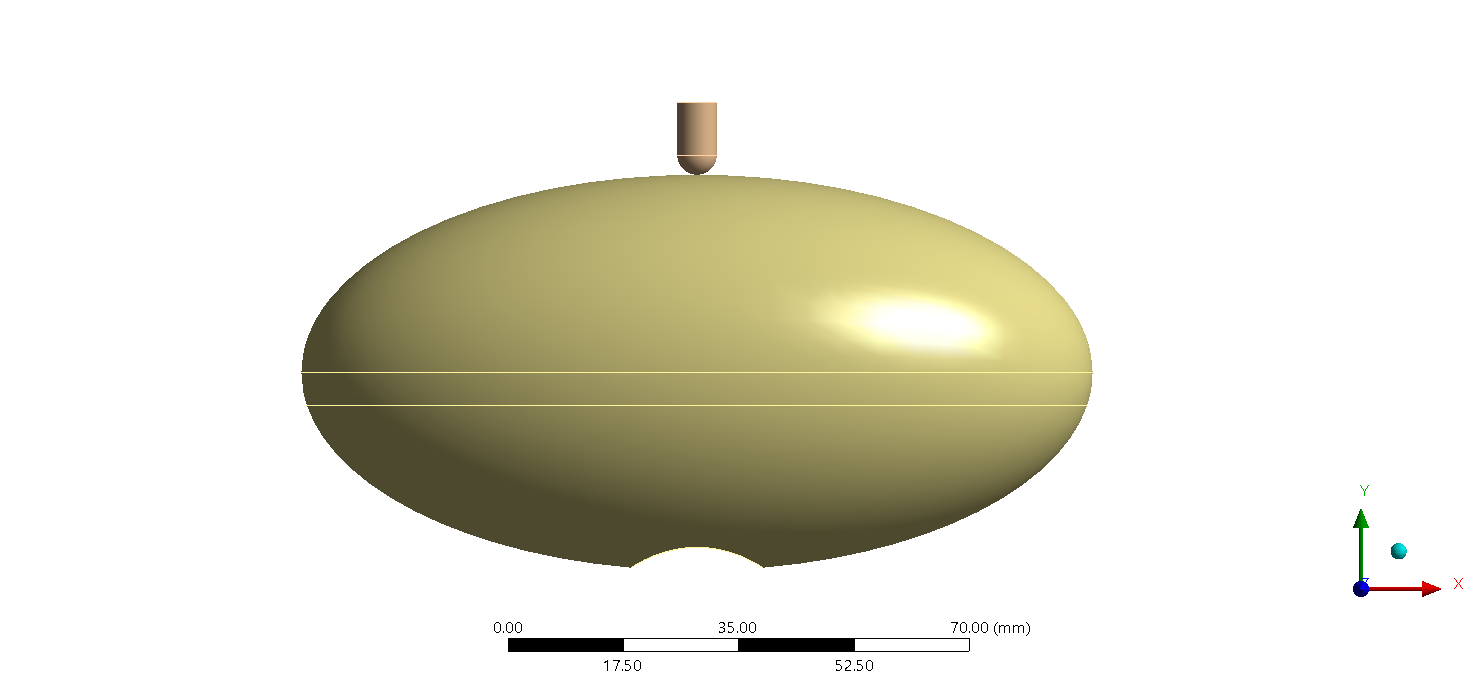
\includegraphics[width=10cm]{Images/computational/Assemblynoplatform2.png}%
   \caption[Computational model I geometry]{CM I geometry: Illustration of the geometry model with its key components, indenter and specimen with tumor extraction.}%
   \label{fig:geometrycpI}%
\end{figure}
%contact
The contact formulation between the indenter and the specimen was set to frictionless (CONTA174) to reduce
overall model complexity and mimic the lubricated contact of the experiment configuration.
The lower half of the specimen was defined as a fixed support, mirroring the physical constraint of the 
experimental setup. The displacement value $h$ was applied to the indenter in the Y-direction,
and the force reaction $F$ was subsequently obtained.\\
%Mesh
A global element size of $e_{I_s}=\SI{5}{\milli\meter}$ was applied to the specimen's mesh, which 
consisted of quadratic tetrahedral elements. The contact area between the indenter and the specimen's surface 
was refined to $e_{I_a}=\SI{0.3}{\milli\meter}$ (Fig.\ref{fig:cpImesh}). The primary reason for applying contact
sizing refinement was to ensure independence from the specimen's geometry or the indenter's position on the specimen's surface.\\
\begin{figure}
    \centering
    \begin{subfigure}[b]{0.45\textwidth}
    \centering
    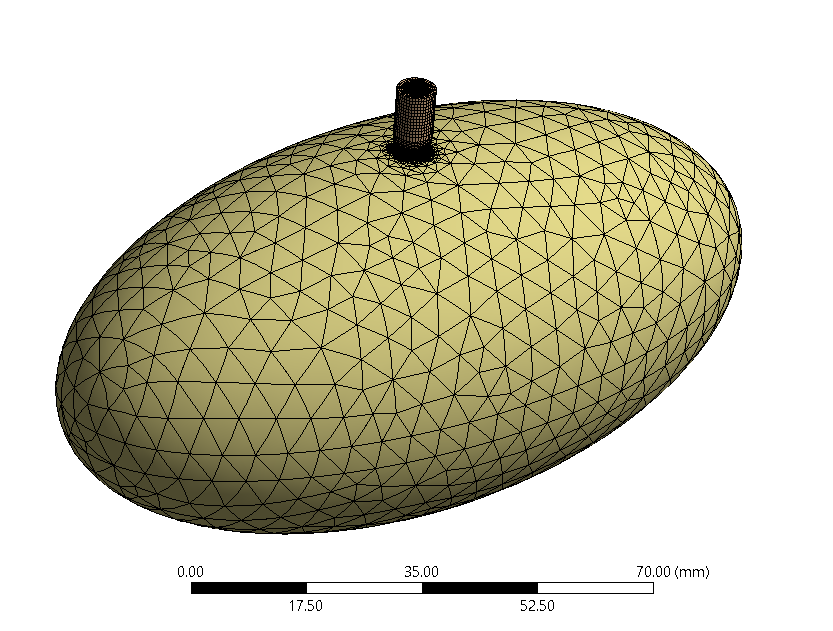
\includegraphics[width=\textwidth]{Images/computational/MeshCSES03total.png}
    \caption{Whole geometry meshing}
    \label{fig:cp1meshtotal}
    \end{subfigure}
    \hfill
    \begin{subfigure}[b]{0.45\textwidth}
    \centering
    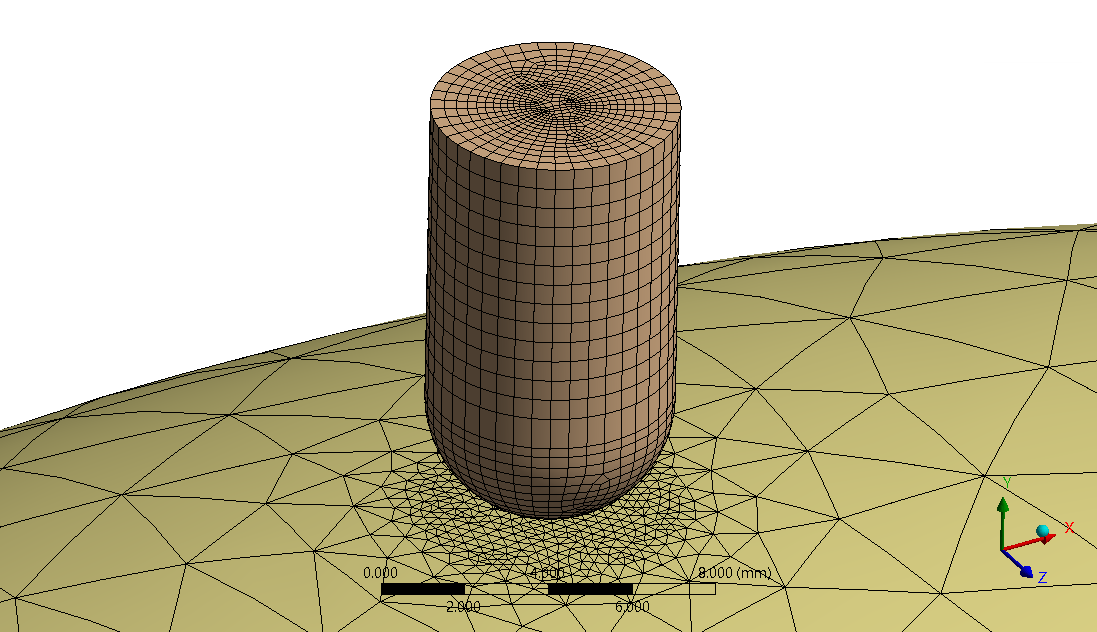
\includegraphics[width=\textwidth]{Images/computational/MeshCSES03.png}
    \caption{Mesh refinement area}
    \label{fig:cp1meshref}
    \end{subfigure}
    \hspace{0.3cm}
    \caption[Computational model I mesh]{CM I mesh: Patch conforming mesh with contact sizing refinement in the contact between the indenter and the specimen's surface.}
    \label{fig:cpImesh}
\end{figure}
Finally, initial parameters were assigned to the computational model to approximate the mechanical properties of ultra-soft polyurethane. 
For the linear elasticity level, values for the Young's modulus $E$ and the Poisson's ratio $\nu$ were assigned. 
From the main assumptions made in Section \ref{section:mainassumption}, the Poisson's ratio for the first 
level material model was set to $\nu_{LE} =  0.49$, and the Young's modulus was calculated using equation \ref{eq:forcelinear}
\begin{align}
    E = \frac{3F(1-\nu^2)} {4{r_i}^{\frac{1}{2}} {h}^{\frac{3}{2}}}\, .
    \label{eq:forcelinearcp1}
\end{align}
Substituting the indenter radius $r_i = \SI{3}{\milli \meter}$ and the indentation depth $h = \SI{3.8}{\milli \meter}$ a Young's modulus $E_{LE}$ was calculated and resulted in 
\begin{align}
    E_{LE} = 0.018 MPa \approx 0.02 MPa \, .
    \label{eq:Elinearcp1}
\end{align}


\subsubsection*{Level 1 Results}
\label{subsection:level1cmI}
An indentation depth of $h = \SI{3.8}{\milli \meter}$ could not be solved with the linear elastic material model. 
Through an iterative process, it was discovered that the linear elastic material model could only be applied 
up to an indentation depth of $h \approx \SI{2}{\milli \meter}$.\\

The initial attempt to match the experimental and simulation data provided a reasonable approximation of the experimental data.
Figure \ref{fig:MPI2mmvsCPILE} demonstrates the comparison between the experimental data and the CM I using a 
linear elastic material model up to an indentation depth of $h = \SI{2}{\milli \meter}$. The CM I curve displayed 
a more pronounced curvature than the experimental data. Additionally, at $u =\SI{0}{\milli \meter}$, 
the experimental curve exhibited a steeper initial slope; however, as the displacement increased, the 
difference in slope between the two curves diminished.\\

This result indicated that for a displacement greater than $u = \SI{2}{\milli \meter}$, the CM I curve would 
lie above the experimental data. Interestingly, it was observed that, despite employing a linear elastic model, 
the force-displacement curve exhibited a nonlinear response. This observation suggested that even a relatively 
simple material model could capture some degree of nonlinearity. 

\begin{figure}%
    \centering
   \quad
    \begin{tikzpicture}[scale=1]
        \begin{axis}[
            xmax=2.2,xmin=0,
            ymin= 0,ymax=0.2,
            %ytick={0,0.1,0.2,...,0.6},
            xlabel={Displacement $u [mm]$},
            ylabel={Force reaction $F_{MP} [N]$},
            grid = major,
            legend pos= north west]
            \addplot+[smooth, no markers, thick] table [y=$Force$, x=Def]{Table/CP1/MPI2mm.dat};
            \addplot+[smooth, no markers, thick] table [y=$Force$, x=Def]{Table/CP1/CP12mmCSfullmodelLE.dat};
            \legend{Experiment I,CM I-LE}
        \end{axis}
    \end{tikzpicture}%
   \caption[Computational model I vs. Experimental data - Linear elasticity]{CM I vs. EM I: Comparison of force-displacement curves between experimental data for Middle Point case and the initial computational model with a linear elastic model for $h = \SI{2}{\milli \meter}$.}%
   \label{fig:MPI2mmvsCPILE}%
\end{figure}


\subsubsection*{Level 2 Results}
\label{subsection:level2cmI}
At the hyperelastic level, the initial parameters for the Neo-Hookean model, 
the shear modulus $\mu$ and the incompressibility parameter $D_1$ were calculated from the Young's modulus $E_{LE}$
and the Poisson's ratio $\nu$ from the linear elastic model. With equations \ref{eq:mucp1}, \ref{eq:bulkmodcp1}, 
and \ref{eq:incomparcp1}, the shear modulus $\mu_{CMI}$ and the incompressibility parameter $D_{1_{CMI}}$
\begin{align}
    \mu_{CMI} = 0.0067 MPa \, ,
    \label{eq:mucp1result}
\end{align}
\begin{align}
    D_{1_{CMI}} = 6 MPa^{-1} \, ,
    \label{eq:d1cp1result}
\end{align}
were calculated, respectively. These parameters were integrated in the model described above. In comparison to 
the linear elastic model, the Neo-Hookean material model could solve the simulation for an indentantion depth of 
$h =  \SI{3.7}{\milli \meter}$.
\begin{figure}%
    \centering
   \quad
    \begin{tikzpicture}[scale=1]
        \begin{axis}[
            xmax=4.2,xmin=0,
            ymin= 0,ymax=0.6,
            ytick={0,0.1,0.2,...,0.5},
            xlabel={Displacement $u [mm]$},
            ylabel={Force reaction $F_I [N]$},
            grid = major,
            legend pos= north west]
            \addplot+[smooth, no markers, thick] table [y=$Force$, x=Def]{Table/Middle Point/MPI38mm.dat};
            \addplot+[smooth, no markers, thick] table [y=$Force$, x=Def]{Table/CP1/CP1CSfullmodelNH.dat};
            \legend{Experiment I,CM I-NH}
        \end{axis}
    \end{tikzpicture}%
   \caption[Computational model I vs. Experimental data - Neo-Hookean]{CM I vs. EM I: Comparison of force-displacement curves between experimental data for Middle Point case and the initial computational model with a Neo-Hookean model for $h = \SI{3.8}{\milli \meter}$.}%
   \label{fig:MPIvsCPINH}%
\end{figure}
The Neo-Hookean simulation curve displayed a similar slope at lower values of $u$ in comparison to the experimental data.
As the displacement $u$ increased, the difference in slope between the two curves increased, and from $u \approx \SI{2.5}{\milli \meter}$
until the end, the computational curve showed a flatter slope than the experimental curve.\\

Despite the discrepancies between the two curves, the Neo-Hookean provided a fair approximation to the experimental data, considered the 
given displacement range. Likewise, this outcome evidenced that the Neo-Hookean model was capable of capturing some of the nonlinear 
response observed in the experimental data, by directly inputing the calculated values from the linear elastic material model.
Nevertheless, it is important to note that improvements to the computational model are necessary to achieve a more
accurate representation of the experimental results.

\subsection{Nearby Point}
For the nearby point test configuration described in Subsection \ref{subsection:nearbypoint} was also modeled to gain an insight 
of the first set material parameters obtained from the middle point computational model.
For the nearby point computational model, the Neo-Hookean model was employed, and the CM I was adapted by changing the 
indenter's position.

The experimental data curve from \ref{subsection:nearbypointresult} and the computational model's curve are shown in Figure 
\ref{fig:nbpointIvsCPINBNH}. Both curves exhibited a similar parabolic shape; however, the simulation curve showed once again,
at a larger indentation depth, a flatter slope than the experimental data. This result presented a 
nearly identical behavior to that of the middle point case.\\
\label{subsection:nbpcpI}
\begin{figure}%
    \centering
   \quad
    \begin{tikzpicture}[scale=1]
        \begin{axis}[
            xmax=4,xmin=0,
            ymin= 0,ymax=0.6,
            ytick={0,0.1,0.2,...,0.5},
            xlabel={Displacement $u [mm]$},
            ylabel={Force reaction $F_I [N]$},
            grid = major,
            legend pos= north west]
            \addplot+[smooth, no markers, thick] table [y=$Force$, x=Def]{Table/Nearby Point/nbexpI.dat};
            \addplot+[smooth, no markers, thick] table [y=$Force$, x=Def]{Table/CP1/NBPCSNHCPI.dat};            
            \legend{Nearby Point, CM I-NBP-NH}
        \end{axis}
    \end{tikzpicture}%
   \caption[Nearby Point: CM I vs. Experimental data - Neo-Hookean]{NBP - CM I vs. EM I: Comparison of force-displacement curves between experimental data for Nearby Point case and the initial computational model with a Neo-Hookean model for $h = \SI{3.8}{\milli \meter}$.}%
   \label{fig:nbpointIvsCPINBNH}%
\end{figure}
In conclusion, while there were differences, the initial calculated values provided a consistent approximation to experimental
data, indicating that the computational model captures the essential features of the material's behavior.
It was decided that further refinements of the material parameters may be necessary to minimize the error between the 
simulated and experimental curves.

%--------------------------------------------------------------------------------------------------------------
\section{Analysis and Complications}
\label{section:challengescm}
\subsection{Verification of the Computational Model}
The verification of the computational model was an important aspect of ensuring the accuracy and reliability of the 
simulation results. One typical approach to verify the model is to conduct a mesh convergence analysis. To 
reduce computational time, symmetry boundary conditions were applied, and one-quarter of CM I was used.

\subsubsection*{Mesh Convergence Analysis}
The mesh convergence FE model utilized a global element size $e_{M_s}=\SI{2}{\milli\meter}$ for the specimen
and $e_{M_i}=\SI{0.3}{\milli\meter}$ for the indenter.
A refinement was made in the area of interest, i.e., the contact area between the indenter and the specimen's surface,
with a sphere radius of $r_{M_a}=\SI{10}{\milli\meter}$ and an element size of $e_{M_a}=\SI{0.5}{\milli\meter}$ (Fig. \ref{fig:meshconvergencecmI}).

\begin{figure}%
    \centering
   \quad
   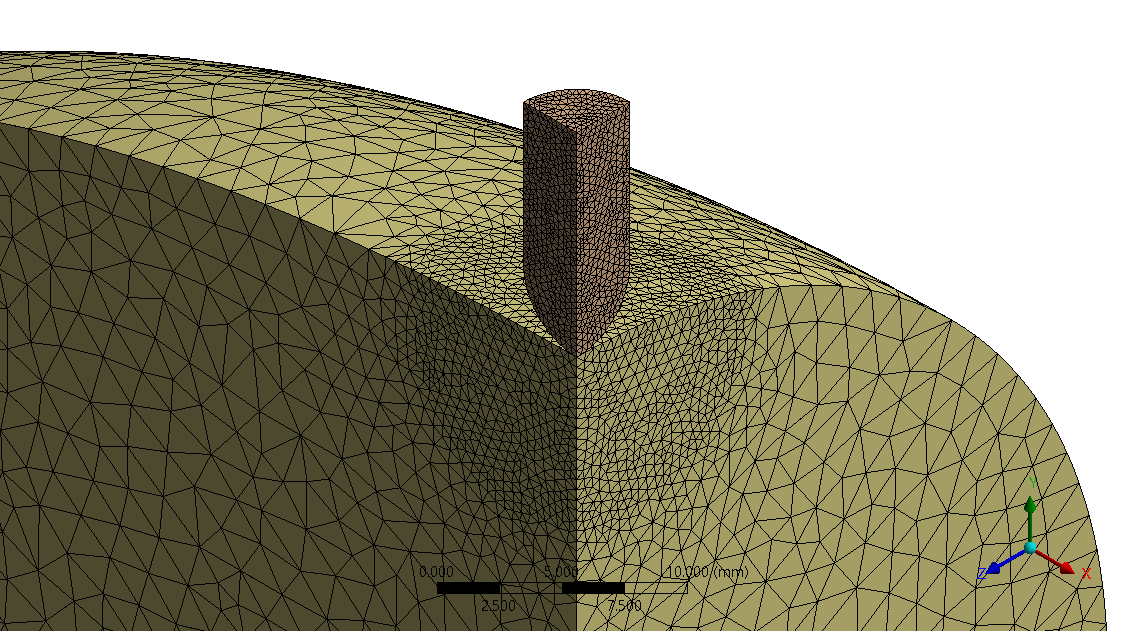
\includegraphics[width=10cm]{Images/computational/meshzoom.png}%
   \caption[Mesh convergence model I]{Mesh convergence analysis I: Mesh refinement strategy in the contact between the indenter and the specimen's surface using one-quarter of the model.}%
   \label{fig:meshconvergencecmI}%
\end{figure}

The mesh convergence analysis presented challenges, as reducing the element size from \SI{5}{\milli\meter} to 
\SI{0.1}{\milli\meter} in the contact area led to unsolvable cases due to large element deformation problems, 
or resulted in values deviating significantly from the expected convergence trend. However, a certain tendency 
towards convergence was observed.

\subsubsection*{Stress Distribution Analysis}
The second challenge encountered during the verification process was the analysis of the stress distribution in 
computational model I. A classic indentation solution between an almost rigid body and an elastic body gives a Hertzian 
solution \cite{Lin2009}. The expected Hertzian stress distribution was not clearly observed; instead, the stress 
contour plot showed rough borders, with some irregularities in the indentation surface area. This issue highlighted
the need for model improvement (Fig. \ref{fig:stressdistributionanalysis}).

Of interest was to observe a cleaner Hertzian stress distribution in the mesh convergence FE model as shown in Figure, 
suggesting that the original model was not entirely reliable and the mesh dependency in the contact area.  

\begin{figure}
    \centering
    \begin{subfigure}[b]{0.45\textwidth}
    \centering
    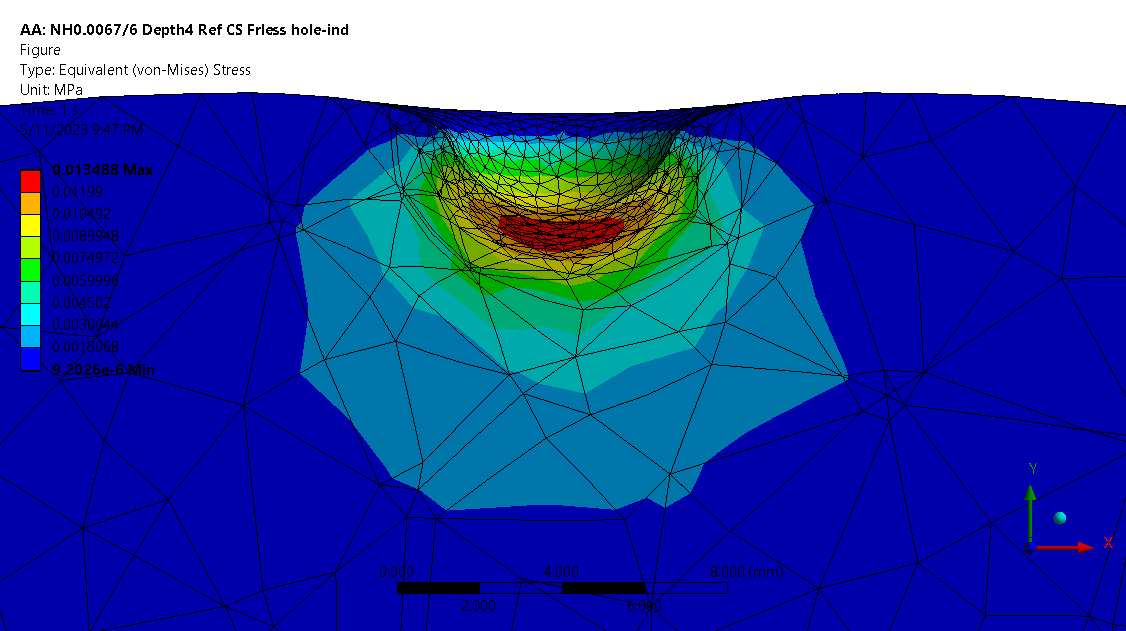
\includegraphics[width=\textwidth]{Images/computational/37CSNHstresshalfzoommesh.png}
    \caption{CM I - NH}
    \label{fig:cm1meshtotal}
    \end{subfigure}
    \hfill
    \begin{subfigure}[b]{0.45\textwidth}
    \centering
    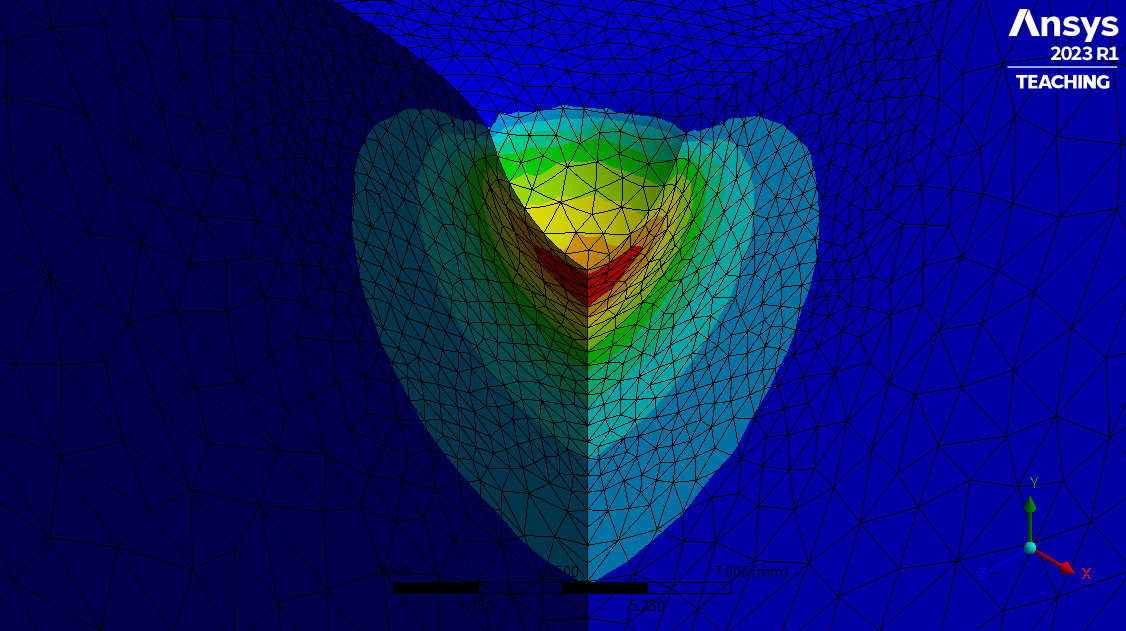
\includegraphics[width=\textwidth]{Images/computational/meshzoomstress.png}
    \caption{Mesh convergence model}
    \label{fig:cm1meshref}
    \end{subfigure}
    \hspace{0.3cm}
    \caption[Mesh convergence model I stress distribution]{Stress distribution analysis of the CM I with a Neo-Hookean material model and the mesh convergence model, which shows the irregularities in the stress contour plot.}
    \label{fig:stressdistributionanalysis}
\end{figure}
%----------------------------------------------------------------------------------------------------------------------
\section{Computational model II}
The computational model II or improved computational model, addressed the challenges and observations 
encountered during the development of CM I. This refined model integrated the proposed
solutions to the previously identified irregularities, and thus served as the final model for the 
iFEM approach for parameter identification. 

\subsection{Middle Point}
\label{subsection:mpcmII}
\subsubsection*{Description}
%geometry and contact
The CM II is the FE model of the experimental model II. The geometry model remained similar to CM I,
featuring a spherical indenter and specimen. The tumor extraction characteristic was omitted, as the 
lower part of the specimen was deemed irrelevant for the overall results (Fig. \ref{fig:cm2meshtotal}). Furthermore, in CM II, only 
one-half of the model was used, again taking advantage of the symmetry boundary conditions. Also,
this choice was made to facilitate the visualization of the deformation profile for subsequent validation 
steps. Same as in CM I, the contact set as frictionless, and the fixed support was applied to the lower part of the organ.\\

%mesh 
The mesh refinement for CM II was guided by the results of the mesh convergence analysis of CP I.
The global element size was maintained at $e_{{II}_s}=\SI{5}{\milli\meter}$, while the refinement area
was adjusted to $e_{{II}_a}=\SI{0.5}{\milli\meter}$ with a sphere radius of $r_{{II}_a}=\SI{8}{\milli\meter}$.
The results in CM I showed that the indenter could be considered as a rigid body; therefore, the element size was 
set at $e_{{II}_i}=\SI{1}{\milli\meter}$, as it did not have a significant influence on the results.
To further improve the mesh quality, a patch independent method was employed, reducing the mesh's 
maximum skewness from \SI{0.85}{} to \SI{0.6}{} (Fig. \ref{fig:cm2meshref}).
\begin{figure}
    \centering
    \begin{subfigure}[b]{0.45\textwidth}
    \centering
    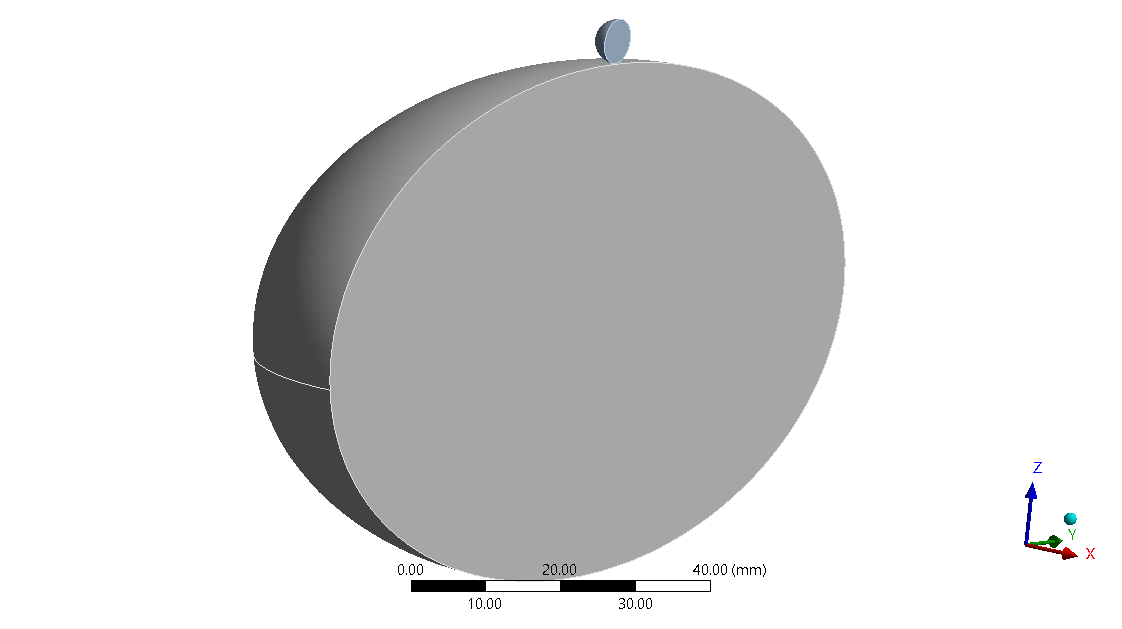
\includegraphics[width=\textwidth]{Images/computational/cm2geometry.png}
    \caption{Geometry model}
    \label{fig:cm2meshtotal}
    \end{subfigure}
    \hfill
    \begin{subfigure}[b]{0.45\textwidth}
    \centering
    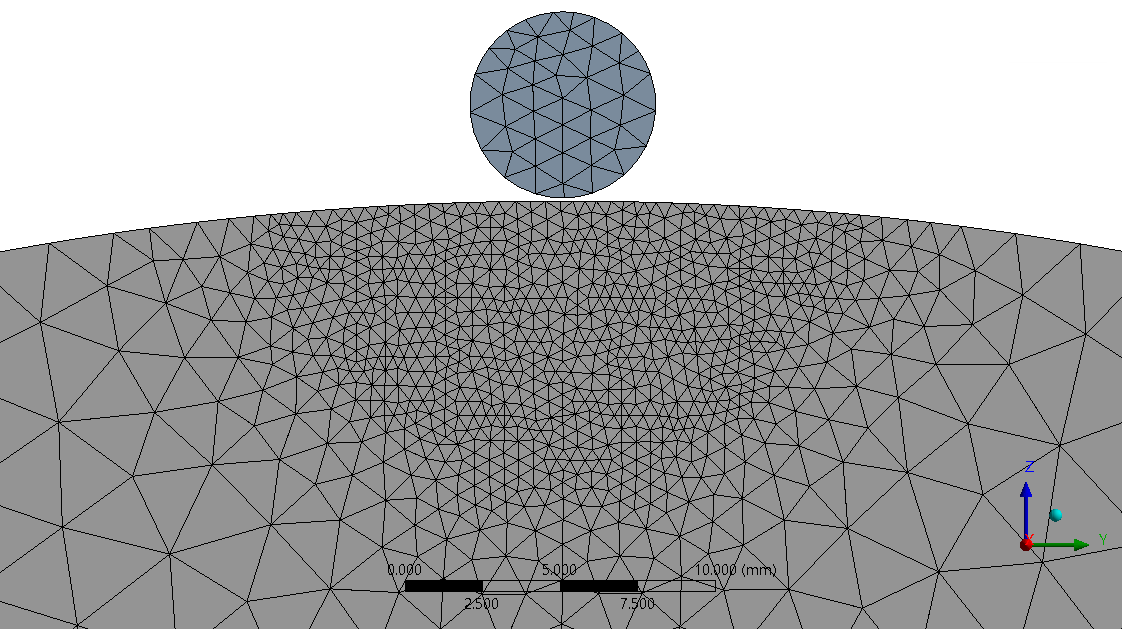
\includegraphics[width=\textwidth]{Images/computational/cm2meshzoom.png}
    \caption{Mesh refinement area}
    \label{fig:cm2meshref}
    \end{subfigure}
    \hspace{0.3cm}
    \caption[Computational model II mesh]{CM II mesh: Patch independent mesh with refinement in the contact area between the indenter and the specimen's surface.}
    \label{fig:cmIImesh}
\end{figure}

\subsubsection*{Large Element Deformation Strategy}
To address the issue of the large element deformation for larger indentation depths, the ANSYS \textbf{nonlinear adaptive region}
option was applied. This feature performed a remeshing operation in the contact area of the specimen whenever 
the elements reached a high distortion level. This adaptive meshing region process made it possible to conduct 
a successful mesh convergence analysis. In this mesh convergence analysis, all values could be calculated and 
convergence was reached. As a result, the element size in the contact area was determined to be changed from 
\SI{0.5}{\milli\meter} to \SI{1}{\milli\meter}. 

\subsubsection*{Stress Distribution Strategy}
In terms of the stress distribution, the computational model II demonstrated improvements over CM I. The new
stress contour plot exhibited more clearly defined borders, and the irregularities present in CM I did not 
emerge on the specimen's indented surface. This resulted in a stress distribution that more closely aligned
with the expected Hertzian solution. A comparative illustration of the stress distributions from CM I and 
CM II is displayed in Figure \ref{fig:cmIIstressdistanalysis}.\\

\begin{figure}
    \centering
    \begin{subfigure}[b]{0.7\textwidth}
    \centering
    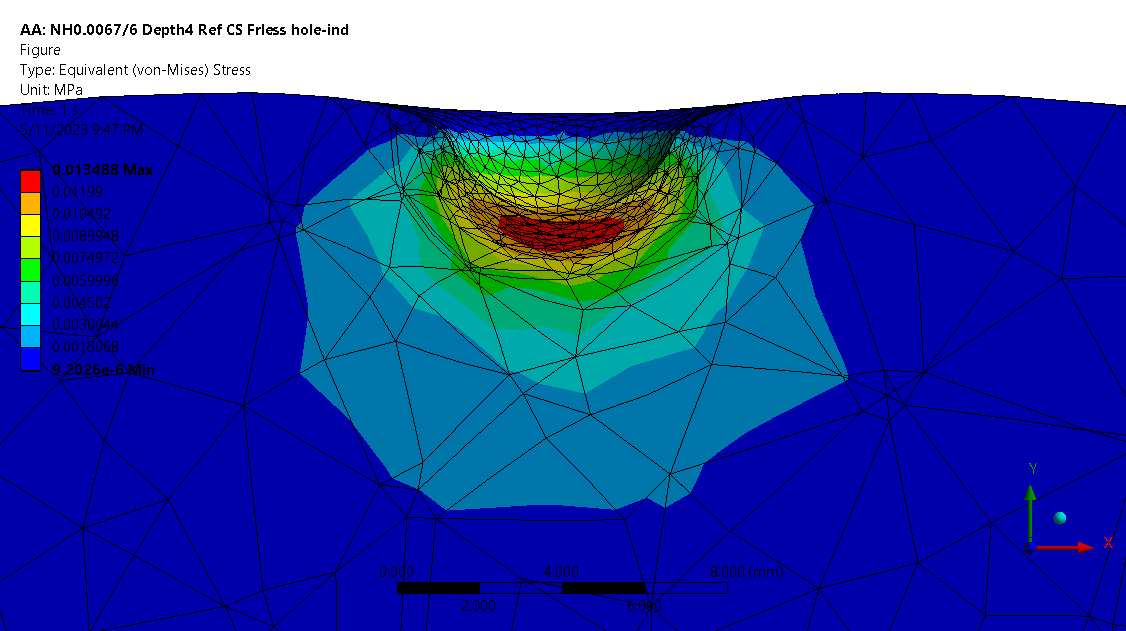
\includegraphics[width=\textwidth]{Images/computational/37CSNHstresshalfzoommesh.png}
    \caption{Computational model I}
    \label{fig:cm1stress}
    \end{subfigure}
    \hspace{0.3cm}
    \begin{subfigure}[b]{0.7\textwidth}
    \centering
    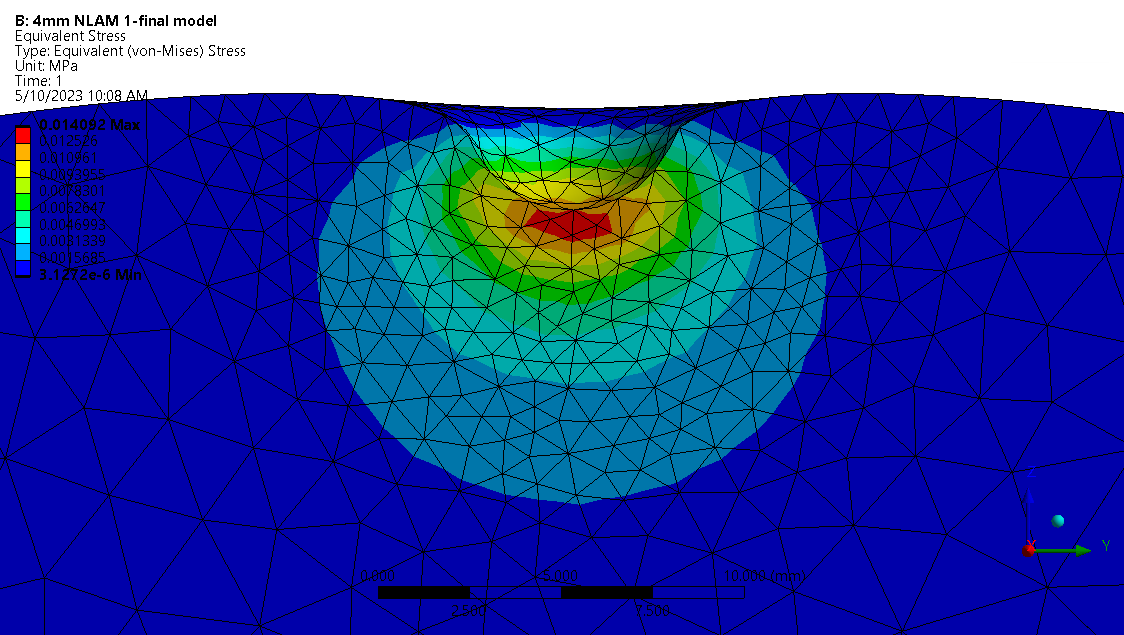
\includegraphics[width=\textwidth]{Images/computational/stresscmII.png}
    \caption{Computational model II}
    \label{fig:cm2stress}
    \end{subfigure}
    \hspace{0.3cm}
    \caption[Stress distribution analysis]{Comparison of stress distribution in computational models I and II with a Neo-Hookean material model after mesh strategy improvements.}
    \label{fig:cmIIstressdistanalysis}
\end{figure}

\subsubsection*{Adjustments to Deformation Behavior}
During the simulated indentation process, an unusual deformation pattern was observed in the computational model.
The indented mass in the model tended to move upwards, enveloping the spherical indenter, which deviated from the 
experimental test observations. In the real-world experiments, the indented mass seemed to 
displace sideways. This discrepancy was attributed to the fixed support boundary condition on the lower specimen's 
surface, which restricted lateral movement of the indented mass.

To improve this unnatural deformation pattern, a more accurate representation of the 
experimental setup was introduced into the FE model. The specimen was positioned on a bowl-shaped
platform, mirroring the experimental configuration. The platform was designed with a slightly major radius to allow 
for lateral displacement of the indented mass to avoid over-constraining the specimen. The contact 
between the specimen and the platform was set to frictional, with a friction coefficient of 0.2, and the base of the platform 
possessed a fixed support.

The inclusion of the platform in the FE model had an impact on the deformation in the indentation area, 
as it showed a more natural deformation. Also, there was an impact on the load-displacement curve (Fig. \ref{fig:noplatformvsplatform}). 
The curve with platform showed a better fit to the experimental data, as the overall shape of the curve was more 
comparable to the experimental data. Therefore, the FE model with the platform was selected as the final model for computational 
model II.\\
\begin{figure}%
    \centering
   \quad
    \begin{tikzpicture}[scale=1]
        \begin{axis}[
            xmax=4,xmin=0,
            ymin= 0,ymax=0.6,
            ytick={0,0.1,0.2,...,0.5},
            xlabel={Displacement $u [mm]$},
            ylabel={Force reaction $F_I [N]$},
            grid = major,
            legend pos= north west]
            \addplot+[smooth, no markers, thick] table [y=$Force$, x=Def]{Table/Middle Point/MPII4mmtotalap.dat};
            \addplot+[smooth, no markers, thick] table [y=$Force$, x=Def]{Table/CP2/CP2noplatNH8541_5.dat};  
            \addplot+[smooth, no markers, thick] table [y=$Force$, x=Def]{Table/CP2/CP2platNH8541_5.dat};            
            \legend{Middle Point, CM II-No platform, CM II-Platform}
        \end{axis}
    \end{tikzpicture}%
   \caption[CP II: No platform vs. with platform]{NBP - CM I vs. EM I: Comparison of force-displacement curves between experimental data for Nearby Point case and the initial computational model with a Neo-Hookean model for $h = \SI{3.8}{\milli \meter}$.}%
   \label{fig:noplatformvsplatform}%
\end{figure}

This chapter has presented an in-depth analysis of the development and refinement of the computational models I and II, used
for simulating the indentation tests. The transition from CM I to CM II revealed the challenges encountered in an indentation 
simulation model and how significant is handling large element deformation for the mesh quality improvement. 
Specifically, the use of a nonlinear adaptive region facilitated more reliable simulation results, displaying a more 
closely Hertzian solution. This improvement reinforced the model's robustness for the subsequent application in an inverse
finite element method approach for the identification of the material's parameters. Moreover, the adjustment in involving platform
emphasized the importance of incorporating realistic boundary conditions and constraints into the computational model.
%best result with convergence
%Their a two main factors which increases the complexity of the validation of the simulation
%and those are, the contact nonlinearity, and the element distortion due to indentation
% experiment. These issues make the computational time expensive, as it requires to manual 
% solutions for the meshing in the area of importance, and small time steps. 
% For that, the nonlinear adaptive meshing option in ANSYS Workbench was applied, which does a remeshing
% process if the a certain parameter is exceeded.%Revisar explanation of nonlinear adaprive meshing
%Specially, for larger indentation cases, this option shows a more stable model with a good mesh convergence analysis.




% Chapter 4

\chapter{Inverse Finite Element Method for Material Parameter Identification} % Main chapter title
\label{iFEMthesis} % For referencing the chapter elsewhere, use \ref{Chapter1} 

The verification of the computational model in the previous chapter was followed by the implementation
of the Inverse Finite Element Method (iFEM) for material parameter identification.
As outlined in Chapter \ref{chapter:computationalmodel}, the Neo-Hookean material model
was employed due to its ability to describe the behavior of ultra-soft polyurethane over 
the range of the considered deformations. Moreover, in Subsection \ref{subsection:inverseFEMtheory} 
the iFEM importance for identifying material parameters for soft materials was explained.\\

In this chapter the process of parameter identifaction 
using this technique will be detailed. Firstly, the initial parameter estimation process will be discussed, 
followed by the optimization process. This revolved around iteratively refining the material parameters
to achieve the best match to the experimental load-displacement data of EM II. The two methods 
explored were ANSYS Response Surface Optimization (RSO) and a custom MATLAB routine. Lastly, the implementation 
and development of these optimization strategies, and their strengths and weaknesses, 
will be discussed. 

%----------------------------------------------------------------------------------
\section{Response Surface Optimization}
The Response Surface Optimization is a technique used in ANSYS for optimizing a design by creating 
a response surface, which represents the relationship between the design variables and the objective 
function or performance criteria. The objective of this feature is to find the optimal set of design 
variables that maximize or minimize the objective function.

The process to find parameters using the RSO in ANSYS generally involves the following steps:
\begin{enumerate}
    \item Define the design variables: The variables that influence the design are identified, e.g., geometric parameter, material properties.
    \item Define objective function: The parameter or objective which is going to be maximize or minimize is defined, e.g., stress, force reaction, volume. 
    \item Define constraints: Constraints or limitations are specified, such as lower or upper bounds.
    \item Generate Design of Experiments (DOE): Set of sample points are generated by varying the design variables. The DOE aims set a design a space efficiently to capture the relationships between the input and output parameters. Simulations are then performed for each set of design variables in the DOE.  
    \item Create a Response Surface: Based on the results of the simulations, the software constructs a surface by interpolating the discrete sampling points from DOE.
    \item Optimize the design: The optimal set of design variables are searched with optimization algorithms by iteratively evaluating the response surface and adjusting the design variables. The default optimization algorithm in ANSYS is the Multi-Objective Genetic Algorithm (MOGA), which supports multiple objectives and constraints. This algorithm aims to find a global optimum for the given problem \cite{Grebenisan2017}.
    \item Verify the candidate points: The given candidate points fro the optimization tool are verified to observe if these satisfy the constraints and meet the target criteria.
\end{enumerate}

For this research the design or input variables were the material properties from the Neo-Hookean 
material model, the shear modulus $\mu$ and the incompressibility parameter $D_1$. The outputs parameters 
were the maximum force reaction in Z-direction $F_z$ and the maximum directional deformation in Z-direction $u_z$.

Based on the observation made in Chapter \ref{chapter:experimentalmodel} regarding the impact of the force 
components in EM II, only the values for the Z-direction were considered. Consequently, the other force 
components could be neglected for this particular case. The prioritization of the Z-direction values came from 
their maximal influence on the outcomes.

\subsection*{Initial Parameter Range}
The initial parameter ranges for the input variables of the RSO were established based on literature review.
Ultra-soft polyurethane, depending on its composition can have a wide range of mechanical properties \cite{Wendels2021}.
From the literature review a Young's modulus range for this material was \SIrange{10000}{100000}{\pascal}, and the 
Poisson's ratio range was \SIrange{0.36}{0.49}{}. As derivated in the previous chapter in 
Subsection \ref{subsection:level2cmI} with the equations \ref{eq:mucp1}, \ref{eq:bulkmodcp1}, 
and \ref{eq:incomparcp1}, the shear modulus $\mu$ and the incompressibility parameter $D_1$ ranges were calculated.
The corresponding ranges were \SIrange{3356}{36765}{\pascal} and \SIrange{1}{168}{\mega\pascal\tothe{-1}}, respectively.

\subsection*{Sensitivity Analysis}
The RSO generated a response surface that enabled the perfomance of a sensitivity analysis.
The sensitivity analysis helped identified which design variables had the most impact 
on the objective function or performance metric, i.e. it was possible to observe how much 
an objective change when each input variable changed. By evaluating the sensitivity of the 
function to variations in the design variables, it was possible to prioritize the most 
influencial parameters and understand their influence in the model during the optimization 
process.

This analysis was presented with a response surface and a local sensitivity bar diagram. 
Figure \ref{fig:fullrangelocalsensi} plots the local sensitvity bar diagram for design variables,
$\mu$ and $D_1$ with respect to the output parameters, the maximum force reaction in Z-direction $F_z$ 
and the maximum directional deformation in Z-direction $u_z$. 

\begin{figure}%
    \centering
	\begin{tikzpicture}
	\begin{axis}[
	    ybar,
	    bar width=1cm,
	    ymax=80,
	    xlabel=Parameter,
	    ylabel={Local Sensitiviy (\%)},
	    xtick=data,
	    xticklabels from table={Table/sensitivity/fullrangeplat2points/test.csv}{Name},
	    enlarge x limits=1,
	    width=0.8\textwidth,
	    height=6cm,
	    legend style={at={(0.5,-0.15)},
	    anchor=north,legend columns=-1},
	    ymajorgrids=true,
	    grid style=dashed,
	]
	\addplot table [x expr=\coordindex, y=P3] {Table/sensitivity/fullrangeplat2points/test.csv};
	\addplot table [x expr=\coordindex, y=P5] {Table/sensitivity/fullrangeplat2points/test.csv};
	\legend{Directional Deformation, Force Reaction Z Axis}
	\end{axis}
	\end{tikzpicture}
	\caption[Local sensitivity analysis - Initial parameter range]{Local sensitivity analysis displaying the influence of the shear modulus and incompressibility parameter for the directional deformation and force reaction in Z-direction.}%
	\label{fig:fullrangelocalsensi}%
 \end{figure}



 



\subsection{Sensitivity Analysis}

The sensitivity analysis provided by the RSO shows the relative importance of each input parameter in determining the output responses. The analysis is presented in the form of a Sensitivity Diagram, which plots the influence of each parameter on the outputs.

In this study, the sensitivity analysis can be used to understand how changes in the shear modulus and incompressibility parameter affect the maximum force and maximum directional deformation. This information can guide the refinement of the parameter ranges in the RSO, as well as the selection of the optimization targets.

For example, if the sensitivity analysis shows that the maximum force is highly sensitive to changes in the shear modulus but not the incompressibility parameter, it may be beneficial to narrow the range of the shear modulus in the RSO and focus on optimizing the maximum force.


\subsection{Initial RSO Results}

The initial RSO offered three candidate sets of material parameters, with the shear modulus around 0.11 MPa and the incompressibility parameter values of $50, 112, and 161 MPa^-1$. However, these candidates did not yield a match with the experimental maximum force. Moreover, it was observed that ANSYS tended to offer only the higher values for $D_1$ and ignored the lower half of the range. This led to a decision to refine the parameter ranges further.

\subsection{Refined Parameter Range and Results}

The refined parameter ranges were $[7500 Pa, 9500 Pa]$ for the shear modulus and $[1, 10 MPa^-1]$ for the incompressibility parameter. The new candidates from the RSO had shear moduli around $0.085 MPa$ and incompressibility parameters of $2, 5, and 7 MPa^-1$. The new target for the RSO was then the force reaction for an indentation depth of 3.9 mm, and the Normalized Root Mean Square Error (NRMSE) was calculated manually for each simulation to evaluate the quality of the solutions.

\section{Advanced Optimization Techniques}

The RSO, though useful, was not providing a satisfactory match to the entire load-displacement curve when using only a single point as the optimization target. This motivated the introduction of multiple targets along the curve, specifically the force reactions at 2 mm and 3.9 mm indentation depths. An additional target at 3 mm was also tested.

\subsection{Minimizing the Objective Function}

In addition to the RSO, a separate optimization was conducted in MATLAB to find the global minimum of the objective function. The objective function was defined as the NRMSE, which quantifies the difference between the simulated and experimental responses.

The MATLAB optimization used the data from the RSO to approximate the objective function as a surface in a three-dimensional space. The x-axis represented the shear modulus, the y-axis represented the incompressibility parameter, and the z-axis represented the NRMSE of each simulation.

The MATLAB optimization then used a mathematical algorithm (such as gradient descent or a genetic algorithm) to search this surface for the set of input parameters that minimized the NRMSE. This set of parameters represented the optimal solution that best matched the experimental data.

This was a bit more detailed explanation of those aspects. Please let me know if you'd like to delve into any other specific areas or if you have further queries.


Additionally, an effort was made to find the global minimum of the objective function (the relationship between the input parameters and the NRMSE) using MATLAB. Using data from approximately 40 simulations, a surface was approximated where the x-axis represented the shear modulus, the y-axis represented the incompressibility parameter, and the z-axis represented the NRMSE of each simulation. The Mean Relative Error (MRE) was also calculated for each simulation, and the same surface approximation method was applied.

\section{Evaluation of the Identified Material Parameters}

The material parameters identified through the RSO and the MATLAB-based optimization were introduced into the computational model for evaluation. The performance of these parameter sets was compared against the experimental data to determine their adequacy.


\section{Comparison between RSO and MATLAB Optimization}

Both RSO and MATLAB-based optimization are valuable tools for parameter estimation and can offer unique advantages in different scenarios. Here, we outline the strengths and weaknesses of each method based on the experiences in this study.

\textbf{Strengths of RSO:}

	1. \textit{User-Friendly Interface:} RSO in ANSYS provides a relatively user-friendly interface that does not require advanced knowledge of programming languages. This can make the process more accessible for users who do not have a background in programming.
	2. \textit{Integrated Design:} Since RSO is an integral part of ANSYS, it works seamlessly with the rest of the software package. This integration can streamline the workflow and reduce the likelihood of errors or inconsistencies.
	3. \textit{Sensitivity Analysis:} RSO includes built-in tools for sensitivity analysis, which can provide valuable insights into the relative importance of each input parameter.

\textbf{Weaknesses of RSO:}

	1. \textit{Limited Flexibility:} RSO may offer less flexibility compared to custom-coded MATLAB optimization routines. For example, it might not be possible to use custom objective functions or optimization algorithms.
	2. \textit{Inability to Handle Complex Objective Functions:} RSO can struggle with objective functions that are highly nonlinear, discontinuous, or have multiple local minima.

\textbf{Strengths of MATLAB Optimization:}

	1. \textit{Highly Customizable:} MATLAB allows for highly customizable optimization routines. You can design your own objective function, constraints, and choose from a variety of optimization algorithms.
	2. \textit{Advanced Analysis Tools:} MATLAB provides advanced tools for data analysis and visualization, which can be useful for interpreting the results of the optimization.

\textbf{Weaknesses of MATLAB Optimization:}

	1. \textit{Requires Programming Knowledge:} Unlike RSO, MATLAB-based optimization requires a good understanding of programming, which can be a barrier for some users.
	2. \textit{Separate Workflow:} Since MATLAB is a separate software, it requires an additional step of exporting and importing data between ANSYS and MATLAB. This can add complexity to the workflow.

In conclusion, the choice between RSO and MATLAB optimization depends on the specific requirements of the study, the complexity of the problem, and the resources and skills available. In this study, both methods were used to leverage their unique advantages and to provide a more comprehensive parameter estimation.



%\section{Material Modeling}
%In an ideal and first scenario, this material can be assumed as linear, isotropic, 
%elastic and nearly imcompressible. For this case, there are two main variables, the Young's
%Modulus \(E\), and the Poisson's ratio $\nu$.
%
%%comentario sobre la influencia del bulk modulus y poissons ratio
%From the parametric analysis, it is possible to see that the bulk 
%modulus of this material does not possess a big impact in the FE 
%simulation results. This conclusion combined with the results 
%from the Poisson ratio in the first material model coincide with the 
%statements from Bergström, where it is no vital to know these parameters 
%to obtain accurate FE computational models, as these have limited
%influence on the mechanical response. \cite{Bergström2015} %pag64Bergströom




%----------------------------------------------------------------------------------
%\subsection{Objective Function Optimzation}

%\subsection{Analysis and Comparison of Each Approach}

%---------------------------------------------------------------------------------

% Chapter 5

\chapter{Results} % Main chapter title
\label{chapter:results} % For referencing the chapter elsewhere, use \ref{Chapter1} 

%----------------------------------------------------------------------------------
\section{Overview and Analysis}
Upon applying the RSO and MATLAB optimization to identify the optimal material parameter set, 
multiple sets were calculated. 
Each simulation deployed various Neo-Hookean parameters sets and 
had a unique load-displacement solutions. These load-displacement curves were 
juxtaposed with the experimental data and the RMSE and NRMSE (Equation \ref{eq:rmse} and \ref{eq:nrmse}) was calculated to quantify the quality 
of each solution. To deepen the evaluation, additional performance metrics were incorporated: 
Mean Relative Error (MRE) (Equation \ref{eq:mre}), Mean Absolute Percentage Error (MAPE)
\begin{align}
    \text{MAPE} = \frac{100\%}{n} \sum_{i=1}^{n} \left| \frac{y_i - \hat{y}_i}{y_i} \right| \,,
\end{align}
and  Relative Root Mean Square Error (RRMSE)  
\begin{align}
    \text{RRMSE} = \sqrt{\frac{1}{n} \sum_{i=1}^{n} \left( \frac{y_i - \hat{y}_i}{y_i} \right)^2} \,.
\end{align}
%https://www.analyticsvidhya.com/blog/2021/10/evaluation-metric-for-regression-models/   
Performance metrics are critical for evaluating the predictive accuracy of the computational model.
These metrics provide insights into how well the model's prediction align with the 
experimental data. The combination of these metrics allowed for a more comprehensive 
assessment of all the simulations performance. For instance, the RMSE and NRMSE measured the
absolute deviation of the predicted values from the observed data, providing an overall 
measure of the computational model accuracy. On the other hand, metrics like MRE, MAPE. and 
RRMSE are useful when considering relative errors. These metrics weighed errors in relation
to the actual size of the actual values \cite{Rajagukguk2020}.\\

The simulation results that produced the lowest performance metrics were set aside as possible
optimal candidates. In particular, the parameters with the lowest NRMSE, MRE and RMSRE were  
investigated. Moreover, a set with an elevated incompressibility parameter was chosen for 
analyzing its influence on validation cases.
The parameters that were determined to provide the best fit to the 
experimental data based on these assessments were listed on Table \ref{tab:materialsetbestfit}.
\begin{table}[ht!]
    \centering
    \begin{tabular}{|c|c|c|c|c|c|c|}
    \hline
    Set & $\mu$ (Pa) & $D_1$ (MPa\textsuperscript{-1}) & NRMSE & MRE & RRMSE & Optimization Method\\
    \hline
    1 & 9999.7 & 5.8 & \textbf{0.0339} & 0.1098 & 0.2067 & RSO 2P RR\\
    2 & 9975.2 & 5.3 & 0.0340 & \textbf{0.1097} & 0.2069 & RSO 2P RR\\
    3 & 10200 & 1.1 & 0.0533 & 0.1139 & \textbf{0.1964} & MATLAB Poly 4 MRE\\
    4 & 12453 & 139.3 & 0.0648 & 0.1713 & 0.2592 & RSO 2P FR\\
    \hline
    \end{tabular}
    \caption[Best material parameter sets]{Neo-Hookean material parameter sets that demonstrated the best fit to the experimental data of the EM II.}
	\label{tab:materialsetbestfit}
\end{table}

\subsection*{Assessment of Performance Metrics}
Defining good performance metrics values required a multi-dimensional approach. 
Firstly, the load-displacement curves' visual inspection revealed a close approximation 
to the experimental data (Fig. \ref{fig:bestfitcandidatescurve}).

The load-displacements curves illustrated that the initial slope of EM II was steeper compared to 
all calculated candidate sets. As the displacement increased sets \SI{1}{} through \SI{3}{} intersected 
the experimental curve. Set \SI{1}{} and \SI{2}{} were nearly identical, initially exhibited an increasing 
slope, yet displayed a tendency to flatten towards the end of the curve, intersecting the experimental curve 
a second time.

On the other hand, set \SI{3}{} crossed the experimental curve around $u=\SI{1.5}{\milli \meter}$, showcasing 
a steeper slope relative to the experimental curve. 

Set \SI{4}{} displayed a pronounced curvature at the outset, followed by an increase in steepness of its slope.
However, it remained constantly below throughout the experimental data.\\

%load-displacements results curves comparison
\begin{figure}%
    \centering
   \quad
    \begin{tikzpicture}[scale=1]
        \begin{axis}[
            xmax=4.2,xmin=0,
            ymin= 0,ymax=0.6,
            ytick={0,0.1,0.2,...,0.5},
            xlabel={Displacement $u [mm]$},
            ylabel={Force reaction $F_{II} [N]$},
            grid = major,
            legend pos= north west]
            \addplot+[smooth, no markers, thick] table [y=$Force$, x=Def]{Table/RSO/expdatatop.dat};
            \addplot+[smooth, no markers, thick] table [y=$Force$, x=Def]{Table/results/set199997_58.dat};
			\addplot+[smooth, no markers, thick] table [y=$Force$, x=Def]{Table/results/set299752_53.dat};
            \addplot+[smooth, no markers, thick] table [y=$Force$, x=Def]{Table/results/set310200_11.dat};
            \addplot+[smooth, orange, no markers, thick] table [y=$Force$, x=Def]{Table/results/set412453_1393.dat};
            \legend{EM II-MP,Set 1,Set 2, Set 3, Set 4}
        \end{axis}
    \end{tikzpicture}%
   \caption[Best material parameter sets load-displacement curves]{Visual analysis of the load-displacement curves of the best material parameter sets with the lowest NRMSE, MRE, and RRMSE and the experimental data.}%
   \label{fig:bestfitcandidatescurve}%
\end{figure}

In addition to the visual analysis, the mean of the performance metrics for all models were calculated and 
compared to its lowest value. Similarly, a baseline model of each performance metric was calculated and 
also compared to the candidate sets (Table \ref{tab:performancegoodness}). 

To clarify, the lowest value of the NRMSE was $\SI{0.0339}{}$. The mean NRMSE across all models was 
$\SI{0.1662}{}$, suggesting that models with an NRMSE below this value outperformed the average.
Consequently, the baseline NRMSE, represented a simple model predicting the mean load-displacement, was 
$\SI{0.6835}{}$, indicating that models with an NRMSE below this value surpassed the baseline model.\\ 

\begin{table}[ht!]
    \centering
    \begin{tabular}{|>{\centering\arraybackslash}m{2cm}|>{\centering\arraybackslash}m{2cm}|>{\centering\arraybackslash}m{2cm}|>{\centering\arraybackslash}m{2cm}|}
    \hline
    Metric & Set values & Mean & Baseline \\
    \hline
    NRMSE &  0.0339 0.0340 0.0533 0.0648 & 0.1662 & 0.6835 \\
    \hline
    MRE &  0.1098 0.1097 0.1139 0.1713 & 0.2689 & 0.5916\\
    \hline
    RRMSE & 0.2067 0.2069 0.1964 0.2592 & 0.2688 & 0.6835\\
    \hline
    \end{tabular}
    \caption[Goodness of fit]{Comparison of the performance metric of each candidate set with their mean value and baseline model value, extracted from all calculated simulations.}
	\label{tab:performancegoodness}
\end{table}

Given the proximity of the values among all candidates, except for set \SI{4}{}, it was 
initially inferred that utilizing NRMSE as the sole performance metric would be adequate for 
evaluating the goodness of fit in this specific case, an indentation of $h=\SI{4}{\milli \meter}$
at the center of the surface.

\section{Validation of Computational Model}
\label{section:validationcm}
In order to confirm the reliability and effectiveness of the identified material parameters,
two distinct validation cases were performed. 
The first validation case (VC I) involved the alteration of the indentation depth, changing it to 
$\SI{8}{\milli \meter}$ from the original $\SI{4}{\milli \meter}$. This case aimed to assess how 
well the material model could adapt and represent the mechanical behavior with increased deformation.

The second validation case (VC II)  revolved around the deformation profile of the spe-\\cimen. The aim here 
was understand the accuracy in predicting the actual deformation shape of the specimen under 
indentation. This provided deeper insights into the effects of the selected incompressibility
parameters.\\

The experimental models for the validation cases followed the same procedural guidelines 
described in Chapter \ref{chapter:experimentalmodel} for experimental model II. 
Furthermore, for the validation cases only Sets \SI{1}{}, \SI{3}{} and \SI{4}{} were evaluated (Table \ref{tab:materialsetbestfit}).
As set \SI{2}{} demonstrated nearly identical results as set \SI{1}{}, it was not considered for the 
validation process.

\subsection{Deeper Indentation}
\label{subsection:8mm}
The first validation experiment featured an indentation depth of $h_{VC1}=\SI{8}{\milli \meter}$,
doubling the previous indentation depth of $h=\SI{4}{\milli \meter}$ at the center of the specimen's 
surface or middle point. Computational model II, described in Chapter \ref{chapter:computationalmodel},
was used with the adjusted indentation depth (Fig. \ref{fig:stressdis8mm}).\\

\begin{figure}%
	\centering
   \quad
   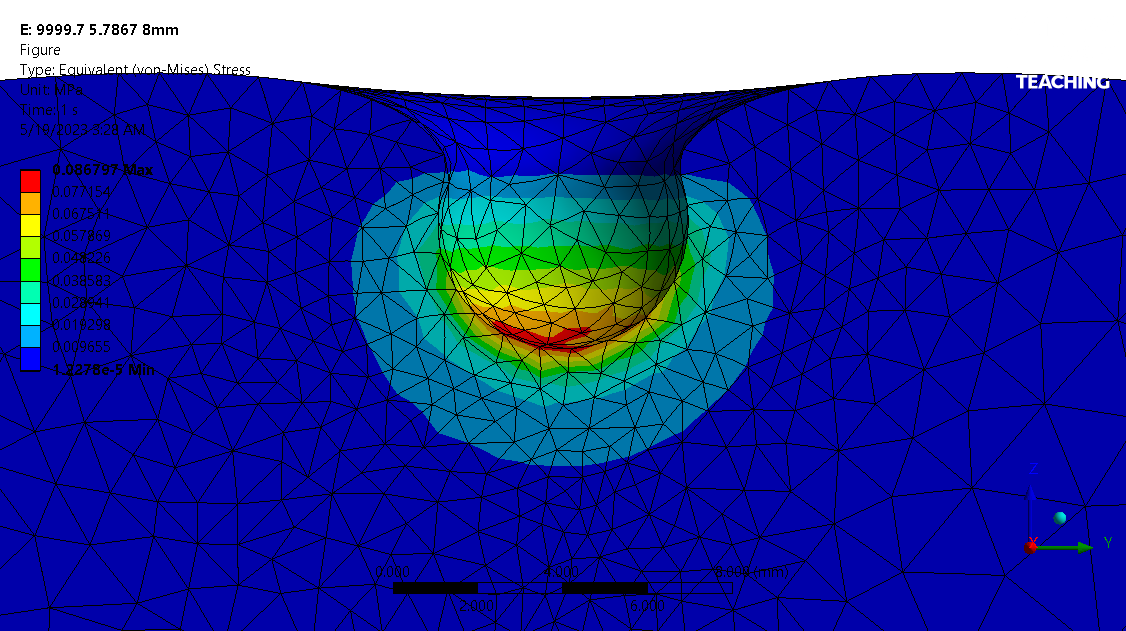
\includegraphics[width=10cm]{Images/validationcase/8mm/setstressdistribution.png}%
   \caption[Deeper Indentation - Stress distribution]{Stress distribution and meshing for the first validation case with an indentation depth of $h_{VC1}=\SI{8}{\milli \meter}$.}%
   \label{fig:stressdis8mm}%
\end{figure}
%Here stress distribution description

To facilitate the comparison of the remaining candidates, the load-displacement curves for the 
set \SI{1}{} with the lowest NRMSE, set \SI{3}{} with the lowest RRMSE, and set \SI{4}{}  with the highest 
incompressibility parameter, were plotted against the experimental data, as shown in Figure \ref{fig:8mmloaddisplcurves}.\\ 
%8mm load displacement curves
\begin{figure}%
    \centering
   \quad
    \begin{tikzpicture}[scale=1]
        \begin{axis}[
            xmax=8.5,xmin=0,
            ymin= 0,ymax=1.5,
            ytick={0,0.2,...,1.4},
            xlabel={Displacement $u [mm]$},
            ylabel={Force reaction $F_{II} [N]$},
            grid = major,
            legend pos= north west]
            \addplot+[smooth, no markers, thick] table [y=$Force$, x=Def]{Table/results/8mm/expdatatop8mm.dat};
            \addplot+[smooth, no markers, thick] table [y=$Force$, x=Def]{Table/results/8mm/set199997_58_8mm.dat};
            \addplot+[smooth, no markers, thick] table [y=$Force$, x=Def]{Table/results/8mm/set310200_11_8mm.dat};
            \addplot+[smooth, no markers, thick] table [y=$Force$, x=Def]{Table/results/8mm/set412453_1393_8mm.dat};
            \legend{EM II-VC I, Set 1, Set 3, Set 4}
        \end{axis}
    \end{tikzpicture}%
   \caption[First validation case load-displacement curves]{Analysis of the load-displacement curves of the best material parameter sets and the experimental data for the first validation case with a deeper indentation.}%
   \label{fig:8mmloaddisplcurves}%
\end{figure}

The load-displacement graph showed that the experimental data displayed again a steeper initial slope 
than the computational models. Sets \SI{1}{} and \SI{3}{} curves intersected the experimental curve 
around a displacement of $u=\SI{2}{\milli \meter}$, whereas set \SI{4}{} intersected at about $u=\SI{3}{\milli \meter}$.

As displacement increased to $u=\SI{4}{\milli \meter}$, the curves for sets \SI{1}{} and \SI{3}{} began 
to flatten and fell beneath the experimental curve, while set \SI{4}{} maintained its steepness and remained above.
At a displacement of $u=\SI{8}{\milli \meter}$, set \SI{4}{} with a maximum force of 
$F_{4_{max}}=\SI{1.3951}{\newton}$ managed to produce the closest 
approximation to the maximum experimental force $F_{II_{max}}=\SI{1.283}{\newton}$.

The new NRMSE values were significantly higher than those of the first case (Table \ref{tab:nrmse8mm}). 
Noteworthy, set \SI{3}{}, with a lower NRMSE for the first case, and set \SI{4}{} with a higher $D_1$ 
exhibited a better NRMSE performance for this case, in contrast to set \SI{1}{}, which had shown 
the best performance for the $h=\SI{4}{\milli \meter}$ indentation.\\

\begin{table}[ht!]
    \centering
    \begin{tabular}{|c|c|c|c|c|}
    \hline
    Set & $\mu$ (Pa) & $D_1$ (MPa\textsuperscript{-1}) & EM II NRMSE & VC I NRMSE\\
    \hline
    1 & 9999.7 & 5.8 & 0.0339 & 0.1503\\
    \textbf{3} & \textbf{10200} & \textbf{1.1} & 0.0533 & \textbf{0.1116}\\
    4 & 12453 & 139.3 & 0.0648 & 0.1425\\
    \hline
    \end{tabular}
    \caption[NRMSE for first validation case]{Comparison of the NRMSE calculated for the EM II and for the first validation case with a deeper indentation.}
	\label{tab:nrmse8mm}
\end{table}

This suggested that the identified parameters may not be able to capture the behavior 
of the material at larger indentations. Therefore, a case-specific parameter identification
for accurate modelling of larger indentations would be required.\\

%------------------------------------------------------------------------------------------------
\subsection{Deformation Profile Analysis}
\label{subsection:defprofanalysis}
The second validation case evaluated the deformation profile of the specimen for the first 
indentation case of $h=\SI{4}{\milli \meter}$ in the middle of the specimen's surface. The goal 
was to understand how the selection of the incompressibility parameter, linked to the 
bulk modulus, influenced the deformation shape under indentation.\\

To capture the deformation shape of the specimen, the displacement of the points along an axis positioned 
$\SI{5}{\milli \meter}$ parallel to the X-axis were calculated (Fig. \ref{fig:defprofdiagram}). %Figure of diagram of
This reference line was chosen to avoid any optical interference caused by the indenter during the 
laser measurements, as illustrated in Figure \ref{fig:defprofinter}.
Figure \ref{fig:defprofexperiment} illustrates the experiment conducted by YNU.
Using the marked points as reference, the laser displacement meter captured the specimen's 
shape along the parallel axis both before and during the indentation process.
This allowed for the measurement of the deformation profile at intervals of $\SI{1}{\milli \meter}$
throughout the indentation until reaching the maximum depth of $\SI{4}{\milli \meter}$ was reached (Appendix \ref{AppendixA}).\\

\begin{figure}%
	\centering
   \quad
   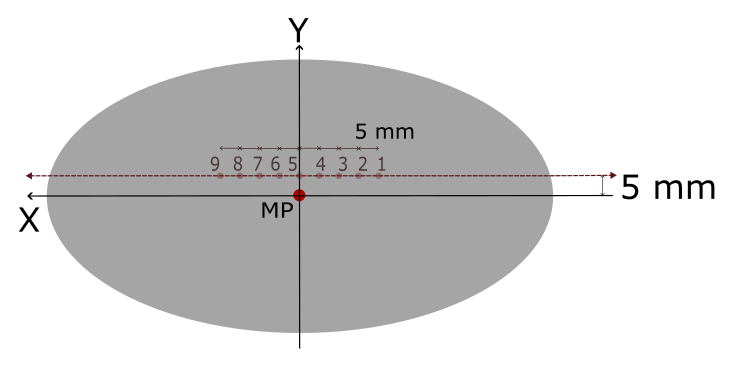
\includegraphics[width=10cm]{Images/validationcase/defprof/defprofdiag.png}%
   \caption[Deformation profile - Diagram]{Deformation profile measurement diagram for the second validation case, showing the measured points along the parallel to X-axis.}%
   \label{fig:defprofdiagram}%
\end{figure}

\begin{figure}
    \centering
    \begin{subfigure}[b]{0.5\textwidth}
    \centering
    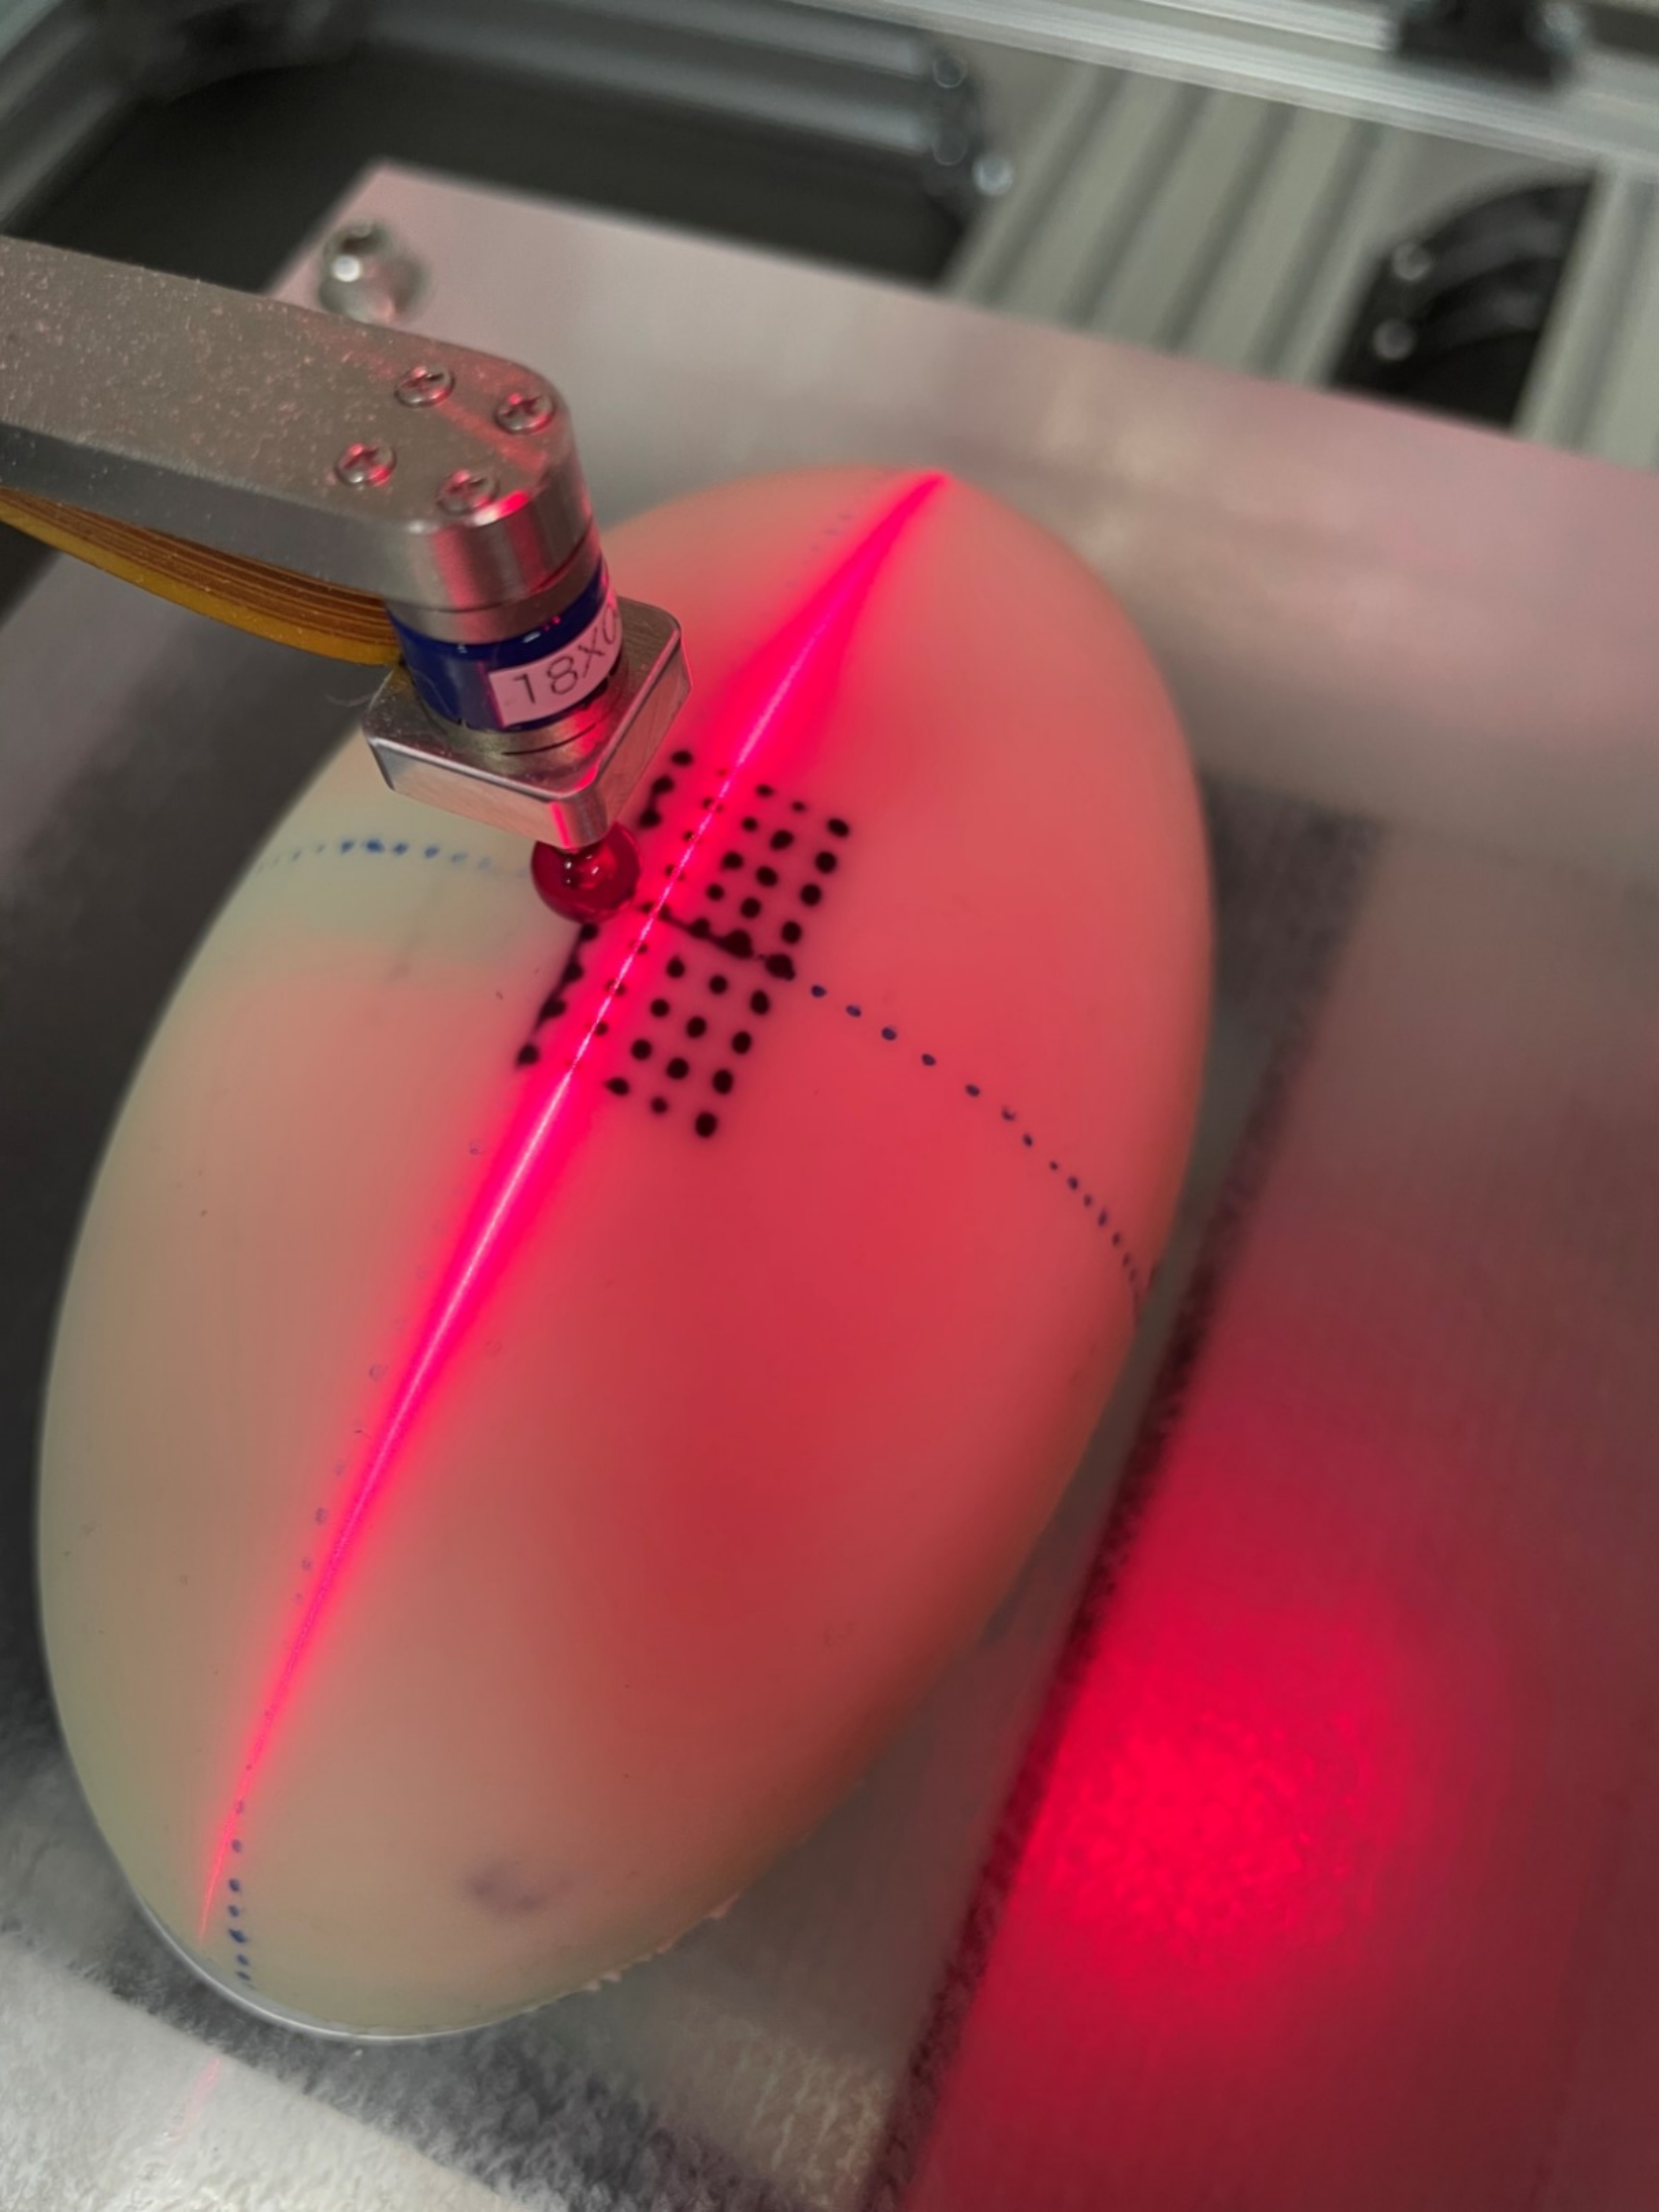
\includegraphics[width=\textwidth]{Images/validationcase/defprof/defprofexp.png}
    \caption{Experimental setup with laser displacement meter measurement}
    \label{fig:defprofexce}
    \end{subfigure}
    \hfill
    \begin{subfigure}[b]{0.5\textwidth}
    \centering
    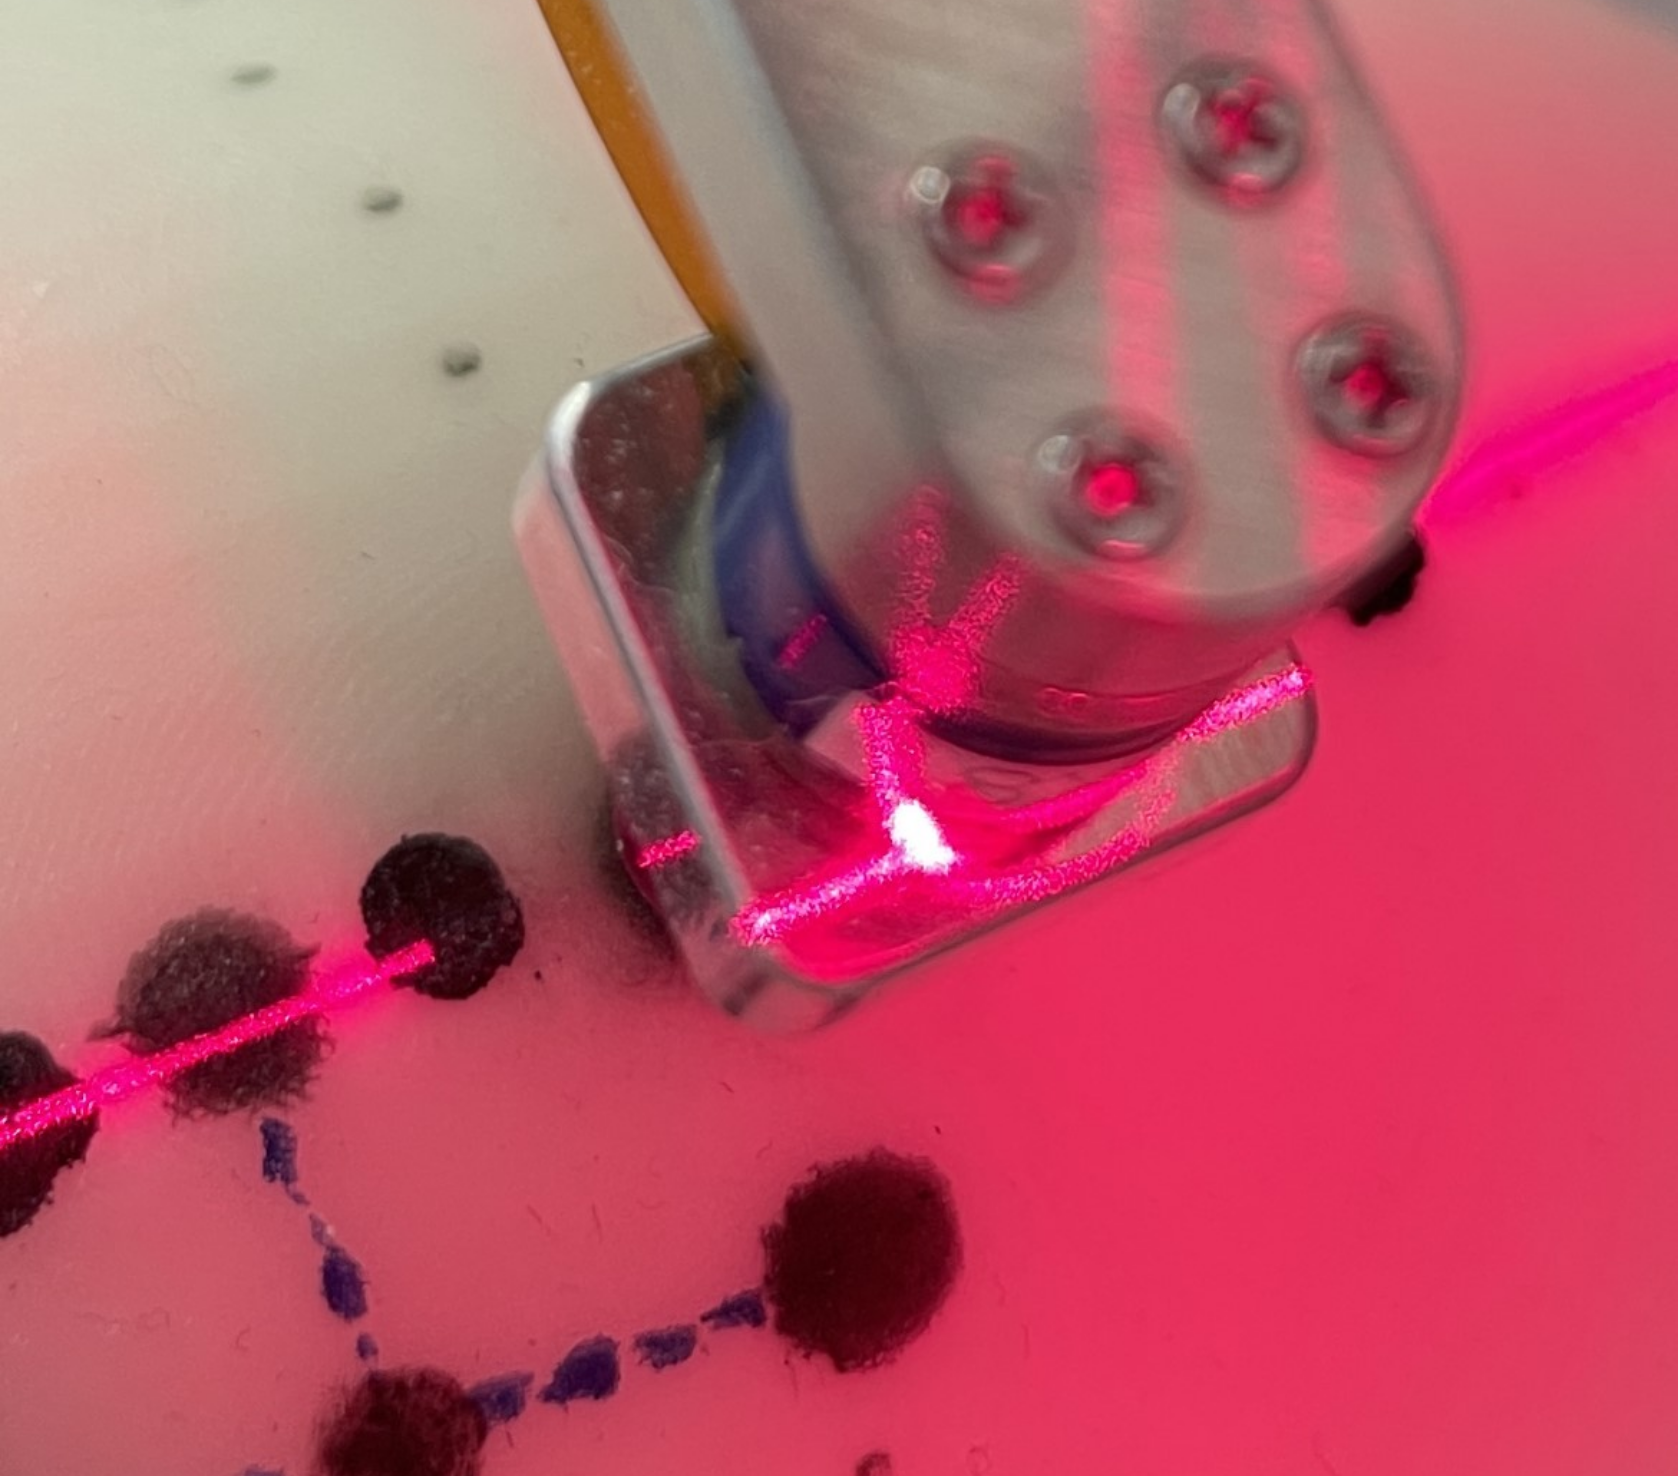
\includegraphics[width=\textwidth]{Images/validationcase/defprof/interferencedef.png}
    \caption{Interference from the indenter of the measurements along the main X-axis}
    \label{fig:defprofinter}
    \end{subfigure}
    \hspace{0.3cm}
    \caption[Deformation profile experiment]{Deformation profile experiment setup performed by YNU to capture the shape of the specimen during the indentation test.}
    \label{fig:defprofexperiment}
\end{figure}

From the results calculated with the computational model II for the middle point case, 
a method to capture the deformation profile for the second validation case was required.
However, tracking specific points on the surface of the simulation was challenging due to 
the remeshing process of the nonlinear adaptive meshing option utilized in the model. This
process did not support the measurement of the displacement for a specific node, as the 
position of the node changed throughout the execution of the model's calculation.\\

To overcome this issue, a section plane was created, located $\SI{5}{\milli \meter}$ to the 
right of the symmetry axis, similar to the experimental model. Probe points were then
selected around the deformed surface within this plane (Fig. \ref{fig:defprofcompmodel}).

\begin{figure}%
	\centering
   \quad
   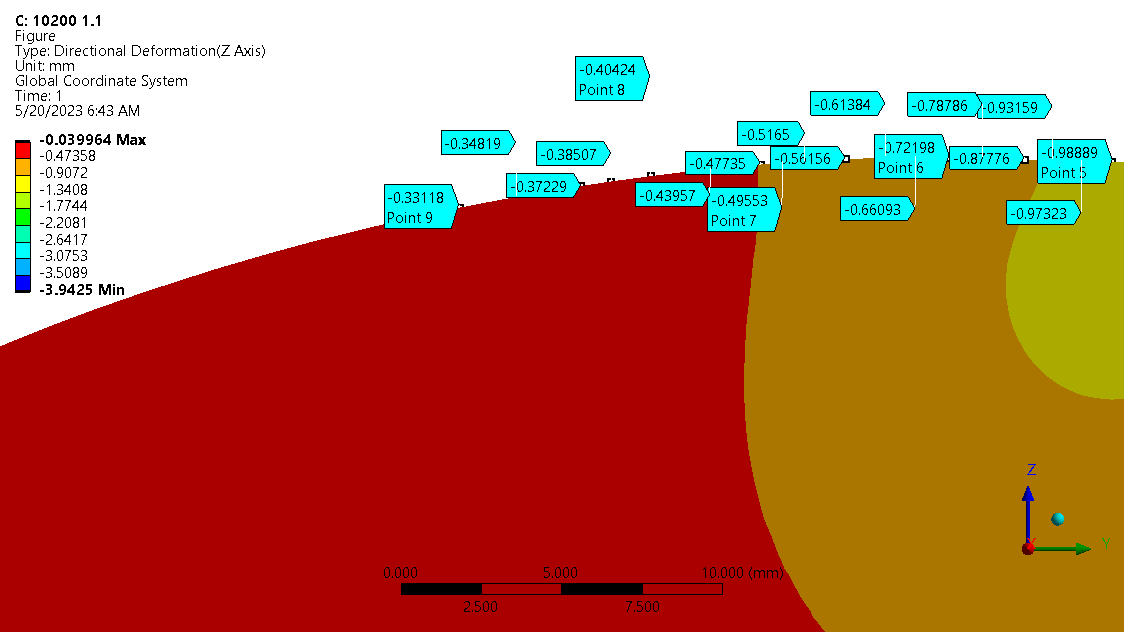
\includegraphics[width=10cm]{Images/validationcase/defprof/10200defprofile.png}%
   \caption[Deformation profile - Computational model]{Deformation profile measurement in the computational model with aid of probes along the surface of the section plane located $\SI{5}{\milli \meter}$ next to the X-axis.}%
   \label{fig:defprofcompmodel}%
\end{figure}

The deformation profiles for the remaining candidate sets were compared with the experimental
data, as shown in Figure \ref{fig:defprofiledata}. Although all computational models 
showed some degree of misalignment with the experimental data, the position of maximum deformation,
Point \SI{5}{} next to middle point, had a close match for sets \SI{1}{} and \SI{3}{}.

Further, as the incompressibility parameter decreased, the overall deformation decreased. The 
NRMSE values for this case were listed on Table \ref{tab:nrmsedefprof}. The NRMSE results 
revealed that the set \SI{3}{} had the best value followed closely by set \SI{1}{}. This validation case 
showcased that the selection of the range set for the iFEM process impacts the deformation response, even though the
influence of the incompressibility parameter on the force reaction results was relatively minor.\\
\begin{table}[ht!]
    \centering
    \begin{tabular}{|c|c|c|c|c|}
    \hline
    Set & $\mu$ (Pa) & $D_1$ (MPa\textsuperscript{-1}) & EM II NRMSE & VC II NRMSE\\
    \hline
    1 & 9999.7 & 5.8 & 0.0339 & 0.3126\\
    \textbf{3} & \textbf{10200} & \textbf{1.1} & 0.0533 & \textbf{0.2810}\\
    4 & 12453 & 139.3 & 0.0648 & 0.5645\\
    \hline
    \end{tabular}
    \caption[NRMSE for second validation case]{Comparison of the NRMSE calculated for the EM II and for the second validation case for the deformation profile curves.}
	\label{tab:nrmsedefprof}
\end{table}

\begin{figure}%
    \centering
   \quad
    \begin{tikzpicture}[scale=1]
        \begin{axis}[
            xmax=25,xmin=0,
            ymax= 0,ymin=-1.4,
            ytick={0,-0.2,...,-1.4},
            xlabel={X-Axis displacement $u_{x} [mm]$},
            ylabel={Z-Axis displacement $u_{x} [mm]$},
            grid = major,
            legend pos= south east]
            \addplot+[smooth, thick] table [y=$Def$, x=Xdis]{Table/results/defprofile/defprofexp.dat};
            \addplot+[smooth, no markers, thick] table [y=$Def$, x=Xdis]{Table/results/defprofile/set1prof.dat};
            \addplot+[smooth, no markers, thick] table [y=$Def$, x=Xdis]{Table/results/defprofile/set3prof.dat};
            \addplot+[smooth, no markers, thick] table [y=$Def$, x=Xdis]{Table/results/defprofile/set4prof.dat};
            \legend{EM II-VC II, Set 1, Set 3, Set 4}
        \end{axis}
    \end{tikzpicture}%
   \caption[Second validation case measurement data]{Analysis of the deformation profile curves of the best material parameter sets and the experimental data for the second validation case.}%
   \label{fig:defprofiledata}%
\end{figure}

Based on the combined results of both validation cases and their NRMSE values, set 3 with a 
shear modulus $\mu=\SI{10200}{\pascal}$ and the incompressibility parameter $D_1=\SI{1.1}{\mega\pascal\tothe{-1}}$ 
was identified as the best overall choice. This material parameter set captured with good 
agreement the indentation for EM II, and showed the best results for the deformation profile 
validation case and the deeper indentation case.  

%--------------------------------------------------------------------------------------------------
\subsection{Nearby Point - Blue Point}
\label{subsection:bluepoint}
After identifying set \SI{3}{} as the best candidate from the initial two validation cases, this 
parameter set was subjected to a third validation test. This experiment was conducted on a 
nearby point, referred to as the blue point (BP), situated at a diagonal distance of approximately $\SI{3.5}{\milli \meter}$ 
from the middle point, as illustrated in Figure \ref{fig:bluepointdiag}.\\%insert diag
\begin{figure}%
	\centering
   \quad
   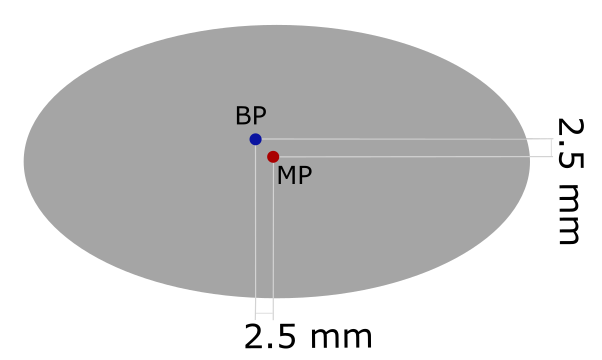
\includegraphics[width=8cm]{Images/validationcase/bluepoint/bluepointdiag.png}%
   \caption[Blue point - Diagram]{Blue point position diagram for the third validation case to evaluate the prediction of all force components.}%
   \label{fig:bluepointdiag}%
\end{figure}
To mimic the conditions of the experimental model II, the indentation depth was kept at $h_{VCIII}=\SI{4}{\milli \meter}$.
Based on the insights acquired from the deeper indentation validation case, it was considered 
prudent to maintain this depth to ensure that the selected material parameters would accurately 
represent the behavior of the specimen for this new indentation point.\\

In this use case, unlike the previous ones, the full computational model was required, as shown in Figure \ref{fig:bluepointcm}.
The symmetry boundary conditions used before were not applicable due to shifted indentation position.
With exception from these conditions the blue point model followed the process as computational model II, described 
in Section \ref{section:cmII}.

\begin{figure}
    \centering
    \begin{subfigure}[b]{0.5\textwidth}
    \centering
    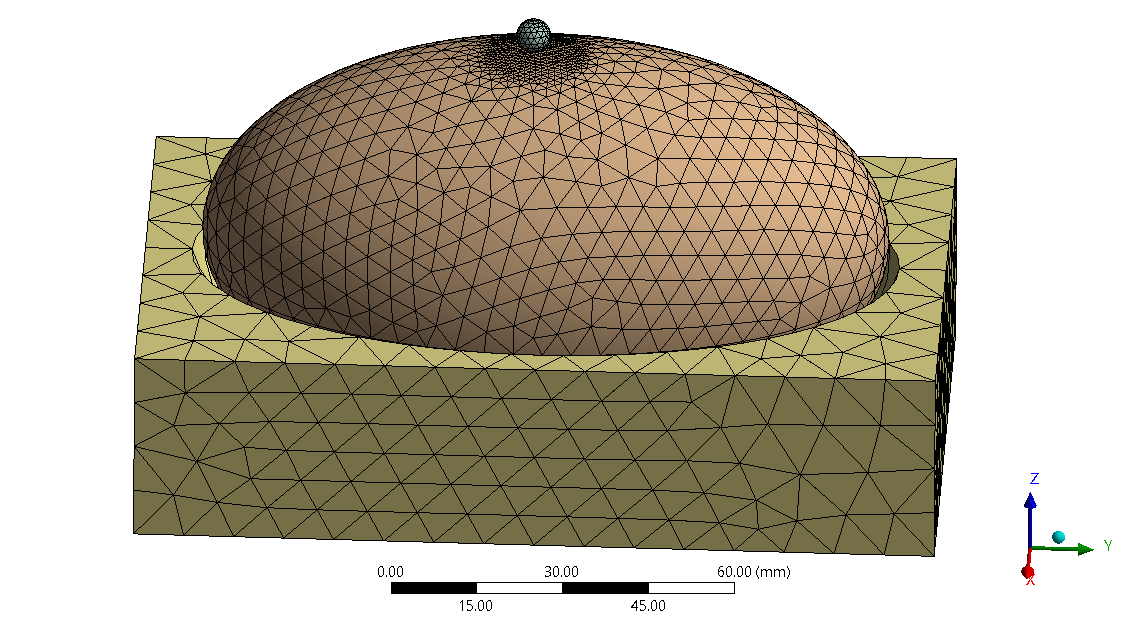
\includegraphics[width=\textwidth]{Images/validationcase/bluepoint/bluepointmesh.png}
    \caption{Full model geometry and mesh}
    \label{fig:bluepointgeoandmesh}
    \end{subfigure}
    \hfill
    \begin{subfigure}[b]{0.5\textwidth}
    \centering
    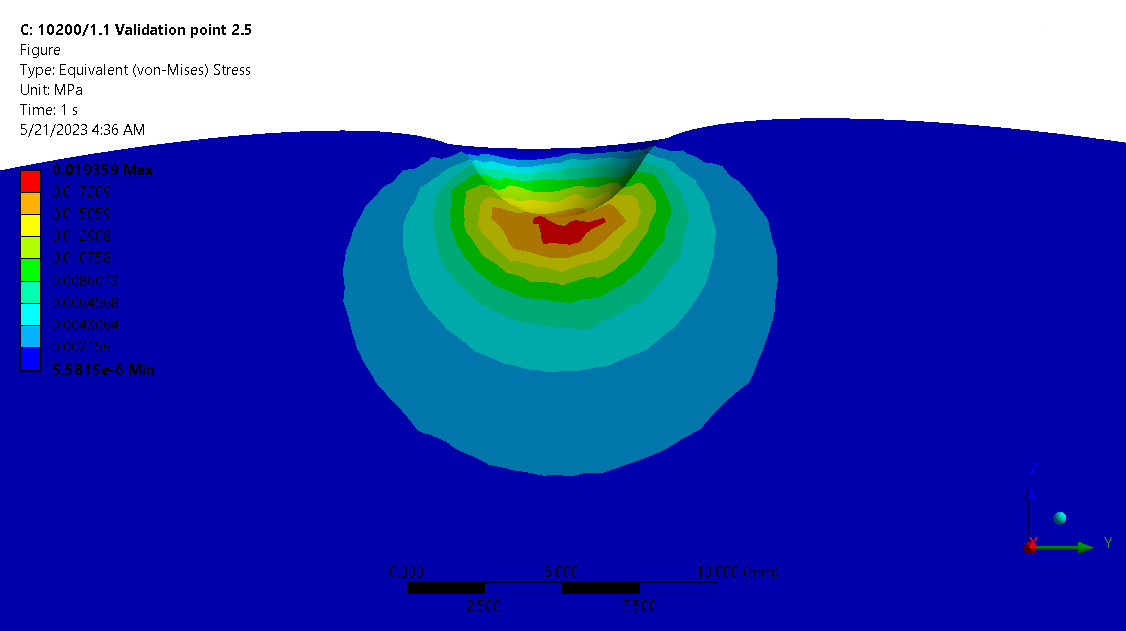
\includegraphics[width=\textwidth]{Images/validationcase/bluepoint/bluepointstress3.png}
    \caption{Von-Mises stress distribution}
    \label{fig:bluepointstress}
    \end{subfigure}
    \hspace{0.3cm}
    \caption[Blue point computational model]{Blue point computational model with use of the full geometry and stress distribution analysis.}
    \label{fig:bluepointcm}
\end{figure}

Furthermore, it was anticipated based on previous nearby point experiments that force components in 
x and y directions would become significant the further the indentation position was from the middle point (Subsection \ref{subsection:nearbypointresult}).
Hence, these components were included in the analysis alongside the z-direction force component.\\

The load displacement curves comparison for the middle and blue point revealed distinct behaviors.
For the middle point in Figure \ref{fig:mpforcecompvc}, the x-force component in the computational model was close to zero,
in comparison to the experimental data, which possessed a small but noticeable peak. 
Moreover, the simulation results for this force component appeared unstable.

On the contrary, the y-force component showed show a clear nonlinear trend in the computational model,
whereas the experimental curve showed minimal variation. The z-force component was previously analyzed 
and used to identify the material parameters, therefore has the closest match between the curves.

The total force curve exhibited a similar initial slope difference as showcased for the z-force component
However, after reaching a displacement of $u\approx\SI{1.2}{\milli \m}$, the simulation curve showed a increased slope,
diverging slightly from the experimental data.\\

The calculated NRMSE for all components and the total force reaction of the middle point test were listed in Table \ref{tab:forcecompnrmse}.
In the table was observed that the components for x and y showed high NRMSE values, but 
the z-component and the total force still lied below or slightly higher than the 
acceptable NRMSE limit of $\SI{0.1668}{}$.\\

\begin{table}[ht!]
    \centering
    \begin{tabular}{|>{\centering\arraybackslash}m{2cm}|>{\centering\arraybackslash}m{2.5cm}|>{\centering\arraybackslash}m{2cm}|>{\centering\arraybackslash}m{2cm}|}
    \hline
    Case & Force & NRMSE  \\
    \hline
    Middle Point & x-component y-component z-component Total & 1.1329 67.984 0.0534 0.1669 \\
    \hline
    Blue point & x-component y-component z-component Total & 0.1281 1.5615 0.0990 0.1015 \\
    \hline
    \end{tabular}
    \caption[Force components NRMSE]{Comparison of the NRMSE of all force components and total force reaction for the middle and blue point cases.}
	\label{tab:forcecompnrmse}
\end{table}

\begin{figure}[htbp]
    \centering
    %Fx
    \begin{subfigure}[b]{0.45\textwidth}
    \centering
    \begin{tikzpicture}[scale=0.78]
        \begin{axis}[
            xmax=4.2,xmin=0,
            ymin= -0.001,ymax=0.008,
            ytick={0,0.002,...,0.008},
            xlabel={Displacement $u [mm]$},
            ylabel={Force reaction $F [N]$},
            grid = major,
            legend pos= north west]
            \addplot+[smooth, no markers, thick] table [y=$Fx$, x=Def]{Table/results/bluepoint/midpoint/expmp.dat};
            \addplot+[smooth, no markers, thick] table [y=$Fx$, x=Def]{Table/results/bluepoint/midpoint/simmp.dat};
            \legend{EM II - MP, CM II - MP}
        \end{axis}
    \end{tikzpicture}
    \caption{X-force component}
    \end{subfigure}
    \hspace{0.3cm}
    \begin{subfigure}[b]{0.45\textwidth}
    \centering
    \begin{tikzpicture}[scale=0.78]
        \begin{axis}[
            xmax=4.2,xmin=0,
            ymin= 0,ymax=0.3,
            %ytick={0,0.1,0.2,...,0.6},
            xlabel={Displacement $u [mm]$},
            ylabel={Force reaction $F [N]$},
            grid = major,
            legend pos= north west]
            \addplot+[smooth, no markers, thick] table [y=$Fy$, x=Def]{Table/results/bluepoint/midpoint/expmp.dat};
            \addplot+[smooth, no markers, thick] table [y=$Fy$, x=Def]{Table/results/bluepoint/midpoint/simmp.dat};
            \legend{EM II - MP, CM II - MP}
        \end{axis}
    \end{tikzpicture}
    \caption{Y-force component}
    \end{subfigure}
    \vspace{0.5cm}
    \begin{subfigure}[b]{0.45\textwidth}
    \centering
    \begin{tikzpicture}[scale=0.78]
        \begin{axis}[
            xmax=4.2,xmin=0,
            ymin= 0,ymax=0.6,
            ytick={0,0.1,0.2,...,0.6},
            xlabel={Displacement $u [mm]$},
            ylabel={Force reaction $F [N]$},
            grid = major,
            legend pos= north west]
            \addplot+[smooth, no markers, thick] table [y=$Fz$, x=Def]{Table/results/bluepoint/midpoint/expmp.dat};
            \addplot+[smooth, no markers, thick] table [y=$Fz$, x=Def]{Table/results/bluepoint/midpoint/simmp.dat};
            \legend{EM II - MP, CM II - MP}
        \end{axis}
    \end{tikzpicture}
    \caption{Z-force component}
    \end{subfigure}  
    \hspace{0.3cm}
    \begin{subfigure}[b]{0.45\textwidth}
    \centering
    \begin{tikzpicture}[scale=0.78]
        \begin{axis}[
            xmax=4.2,xmin=0,
            ymin= 0,ymax=0.6,
            ytick={0,0.1,0.2,...,0.6},
            xlabel={Displacement $u [mm]$},
            ylabel={Force reaction $F [N]$},
            grid = major,
            legend pos= north west]
            \addplot+[smooth, no markers, thick] table [y=$Total$, x=Def]{Table/results/bluepoint/midpoint/expmp.dat};
            \addplot+[smooth, no markers, thick] table [y=$Total$, x=Def]{Table/results/bluepoint/midpoint/simmp.dat};
            \legend{EM II - MP, CM II - MP}
        \end{axis}
    \end{tikzpicture}
    \caption{Total force reaction}
    \end{subfigure}
    
    \caption[Middle point force components comparison]{Middle Point: Comparison and analysis of force components of the experimental data and the computational model.}
    \label{fig:mpforcecompvc}
\end{figure}
%blue point
The blue point case a greater alignment across for the x and y-components and the total force reaction, but
the NRMSE value for the z-component worsened from $\SI{0.0534}{}$ to $\SI{0.09}{}$ (Table \ref{tab:forcecompnrmse}).
In this validation case, the force components showed nonlinear trends in both the 
experimental and computational curves, with the simulation closely matching the
maximum forces obtained experimentally, with exception of the y-component, as 
illustrated in Figure \ref{fig:bpforcecompvc}.
This indicated that the identified parameters in set \SI{3}{} was suitable 
for the blue case as well, in addition to display more stable results for 
all load-displacements curves.\\

\begin{figure}[htbp]
    \centering
    %Fx
    \begin{subfigure}[b]{0.45\textwidth}
    \centering
    \begin{tikzpicture}[scale=0.78]
        \begin{axis}[
            xmax=4.2,xmin=0,
            ymin= 0,ymax=0.015,
            %ytick={0,0.002,...,0.008},
            xlabel={Displacement $u [mm]$},
            ylabel={Force reaction $F [N]$},
            grid = major,
            legend pos= north west]
            \addplot+[smooth, no markers, thick] table [y=$Fx$, x=Def]{Table/results/bluepoint/expbp.dat};
            \addplot+[smooth, no markers, thick] table [y=$Fx$, x=Def]{Table/results/bluepoint/simbp.dat};
            \legend{EM II - BP, CM II - BP}
        \end{axis}
    \end{tikzpicture}
    \caption{X-force component}
    \end{subfigure}
    \hspace{0.3cm}
    \begin{subfigure}[b]{0.45\textwidth}
    \centering
    \begin{tikzpicture}[scale=0.78]
        \begin{axis}[
            xmax=4.2,xmin=0,
            ymin= 0,ymax=0.05,
            %ytick={0,0.1,0.2,...,0.6},
            xlabel={Displacement $u [mm]$},
            ylabel={Force reaction $F [N]$},
            grid = major,
            legend pos= north west]
            \addplot+[smooth, no markers, thick] table [y=$Fy$, x=Def]{Table/results/bluepoint/expbp.dat};
            \addplot+[smooth, no markers, thick] table [y=$Fy$, x=Def]{Table/results/bluepoint/simbp.dat};
            \legend{EM II - BP, CM II - BP}
        \end{axis}
    \end{tikzpicture}
    \caption{Y-force component}
    \end{subfigure}
    \vspace{0.5cm}
    \begin{subfigure}[b]{0.45\textwidth}
    \centering
    \begin{tikzpicture}[scale=0.78]
        \begin{axis}[
            xmax=4.2,xmin=0,
            ymin= 0,ymax=0.6,
            ytick={0,0.1,0.2,...,0.6},
            xlabel={Displacement $u [mm]$},
            ylabel={Force reaction $F [N]$},
            grid = major,
            legend pos= north west]
            \addplot+[smooth, no markers, thick] table [y=$Fz$, x=Def]{Table/results/bluepoint/expbp.dat};
            \addplot+[smooth, no markers, thick] table [y=$Fz$, x=Def]{Table/results/bluepoint/simbp.dat};
            \legend{EM II - BP, CM II - BP}
        \end{axis}
    \end{tikzpicture}
    \caption{Z-force component}
    \end{subfigure}  
    \hspace{0.3cm}
    \begin{subfigure}[b]{0.45\textwidth}
    \centering
    \begin{tikzpicture}[scale=0.78]
        \begin{axis}[
            xmax=4.2,xmin=0,
            ymin= 0,ymax=0.6,
            ytick={0,0.1,0.2,...,0.6},
            xlabel={Displacement $u [mm]$},
            ylabel={Force reaction $F [N]$},
            grid = major,
            legend pos= north west]
            \addplot+[smooth, no markers, thick] table [y=$Total$, x=Def]{Table/results/bluepoint/expbp.dat};
            \addplot+[smooth, no markers, thick] table [y=$Total$, x=Def]{Table/results/bluepoint/simbp.dat};
            \legend{EM II - BP, CM II - BP}
        \end{axis}
    \end{tikzpicture}
    \caption{Total force reaction}
    \end{subfigure}
    
    \caption[Blue point force components comparison]{Blue Point: Comparison and analysis of force components of the experimental data and the computational model.}
    \label{fig:bpforcecompvc}
\end{figure}

In conclusion, the third validation case reinforced the validity of set number
\SI{3}{} as the chosen parameter set for this study. This set 
demonstrated an acceptable level of agreement for all cases with an equal 
indentation depth. Moreover, this validation supported that this material model 
can model the behavior of the polyurethane specimen under indentation, particularly
when considering different locations on the specimen's surface and all 
force components into the analysis.
%--------------------------------------------------------------------------------------------------
\section{Framework Proposal}

%------------------------------------------------------------------------------------------------
\section{Limitations and Implications of the Results}



%\subsection{First Experimental model}
%The chosen experimental technique for the inverse identification for this project was indentation. 
%The test specimen used for this experiment was a ultra-soft polyurethane resin. 
%As shown in Fig.. the specimen possesses a ellipsoidal form with 
%with a minor radius \(r_1\) = 35 mm and a major radius \(r_2\) = 60 mm. This was positioned
% on a fixed platform that suited the ellipsoidal geometry of the 
% specimen to constrain its movement. 
% The specimen was tested in a indentation test configuration with a tensile/compression machine.
% To achieve this congiguration a pin with a rounded head made of structural steel, 
% with a radius of \(r_3\) = 3 mm was attached 
% to the holding grips followed by a force load cell. 
%The result of indentation test was a load-displacement points. The approximated 
%polynomial curve was used as a reference for the material modeling.

%test specimen is loaded at a quasi-static rate

% The measured force reation \(F_1\) data showed a very small number, so the 
% first 50 N load cell displayed a lot of noise in the measurements. 
% Therefore, the load cell was change to 10N to reduce this interference. 
%The 10 N load cell displayed the force-displacement curve of the indenter and the specimen
% in a finer way. Furthermore, in order to get the measurement of the load and 
% unloading process of
% the indentation a displacement sensor was attached to the tensile machine.

% The indentation depth \(h_1\) selected for the first model was 3,8 mm on the middle of the 
% top surface of the specimen. This indentation depth surpasses the pin radius \(r_3\) and 
% was chose arbitriarily to analyze the behavior of the material on the defined position.
 %reference?
 Additionally, it was observed that in soft materials it is easier to capture 
 some parameters with a larger indentation. Some references also observe that with
 indentation depth lower than indenter radius has a lot of noise and do not describe
 th results accurately. %reference?

%\begin{figure}[th]
%    \centering
%    \begin{tikzpicture}
%        %\pgfplotsset{%legend outside the plot
%        %every axis legend/.append style={ at={(1.05,0.95)}, anchor=north west,legend columns = 1}}
%        \begin{axis}[
%            %axis lines=middle,
%            %x label style={at={(axis description cs:0.5,-0.1)},anchor=north},
%            %y label style={at={(axis description cs:-0.1,.5)},rotate=90,anchor=south},
%            xlabel={Displacement $u [mm]$},
%            ylabel={Force reaction in Z-Axis $F_z [N]$},
%            legend pos= north west]
%            
%            \addplot+[smooth, mark size = 1pt] table [y=$Force$, x=Def]{Table/data1.dat};
%            %\addplot+[smooth] table [y=Force, x=$Def$]{Table/data2.dat};
%            \legend{Experimental data}%,$l_2$}
%        \end{axis}
%    \end{tikzpicture}
%    \caption[Expdata]{Experimental Load-displacement curve.}
%    \label{fig:testgraph2}
%\end{figure}

%\subsection{Second Experimental model}
%The second experimental model was developed by Yokohama National University. Similar to 
%the first experimental model the test specimen and the platform were it lies, has the 
%same dimensions, minor radius $r_1 = \SI{35}{\milli \m}$ and a major radius \(r_2\) of 60 mm. The
%test specimen is also made from the same material, ultra-soft polyurethane resin.
%
%The indenter on the other hand, is a sphere made of ruby, the sphere radius is also 
%equal to the radius of the pin \(r_s\) 3 mm and attached to it, is the force load cell.
%
%A laser is used to measure the displacement which results in a load-displacement curve.
%With this model it is possible to not only determine the toal force reaction, but also
%it's components \(F_x\),  \(F_y\) and \(F_z\). Furthermore, with the laser it is also
%possible to observe the deformation not only in one point but around the whole area. 
%This allows as to analyze the deformation of the whole structure.
%
%The indentation speed selcted was % ask for which speeed
%and with an indentation depth of \(h_s\) is 4 mm. With this experiment, 4 key points on 
%the sepcimen's surface were chosen: First, in the middle and three other points, one to right, 
%one down, and one diagonal to middle, forming a square with a distance between points 
%of \(d_s\) 20 mm. %add figure with points

%----------------------------------------------------------------------------------
%\section{Material model framework assumptions}
%
%The first point to be analyzed, which is used to build a material model is point No. 1,
%in the middle of the surface. The advantages from this case, is the less influence of
%external factors. For this case it is vaiable to assumed, that shear stresses can be 
%neglected and offers a simple model to focus on the material definition.
%
%For this project, there is a focus on the limitation of each material model, 
%departing from an ideal scenario. From this point on the material will be build 
%accordingly and for each model the influence of the material parameters is going
%to be assessed.


%----------------------------------------------------------------------------------
\section{Material model}

%n an ideal and first scenario, this material can be assumed as linear, isotropic, 
%lastic and nearly imcompressible. For this case, there are two main variables, the Young's
%odulus \(E\), and the Poisson's ratio $\nu$.

%comentario sobre la influencia del bulk modulus y poissons ratio
From the parametric analysis, it is possible to see that the bulk 
modulus of this material does not possess a big impact in the FE 
simulation results. This conclusion combined with the results 
from the Poisson ratio in the first material model coincide with the 
statements from Bergström, where it is no vital to know these parameters 
to obtain accurate FE computational models, as these have limited
influence on the mechanical response. \cite{Bergström2015} %pag64Bergströom

%---------------------------------------------------------------------------------
% Chapter 6

\chapter{Conclusion and Outlook} % Main chapter title

\label{Chapter7} % For referencing the chapter elsewhere, use \ref{Chapter1} 

%----------------------------------------------------------------------------------
\section{Summary and Contributions}
The goal of this study was the identification of soft material parameters through 
an iFEM process. Furthermore, this work focused on developing a framework for identifying the 
essential material parameters of soft materials, particularly, those that experience 
large deformations and display nonlinear responses. The aim of this framework was the 
approximation of the behavior of such complex materials via a simplified material model. 
Moreover, this approach's purpose was to potentially apply this framework in medical research,
particularly for the identification of the material parameters of organs.\\

To fulfill this goal, a combination of both experimentation, performed primarily by Yokohama National University, 
and simulation was utilized. The experiments were conducted to collect load-displacement data from
a representative material sample, ultra-soft polyurethane. A computational model was then 
established, mirroring the physical experiment setup, and an initial guess of the material 
parameters was input.\\

In establishing the computational model, the primary challenge encountered was the 
high distortion effect of elements during simulation calculations. To address this issue, the nonlinear adaptive 
meshing option solution was applied, facilitating the verification of the designed 
computational model. Regarding the material model, varying the levels from linear elasticity to 
Neo-Hookean were explored. In this process, the key parameters were identified, and their interrelationships were analyzed.\\

A Response Surface Optimization (RSO) algorithm was employed to optimize these 
parameters, which were assessed by a performance metric defined as the difference between the 
experimental and simulated results. The RSO method allowed the identification and analysis of the 
key design parameters and their influence on the material's behavior. 
To enhance the RSO results, various performance metrics were calculated and examined for 
the top candidates. This evaluation was conducted to determine if the same material could be approximated 
with different sets of material parameters. Additionally, the approximated polynomial derived 
from the material parameter sets and their corresponding performance metric aided in evaluating the 
candidates yielded by the RSO, which confirmed the correctness of the setup.\\

Moreover, three validation cases were conducted to evaluate the material parameter identification 
approach's robustness. While these cases affirmed the effectiveness of this approach under 
specific conditions, it also revealed inherent limitations. These limitations served to 
lay out the boundaries of this approach's applicability, providing valuable insights for the 
optimization of this framework for future research.

\section{Recommendations for Future Research}
Future research should consider extending and improving the applicability of the developed 
framework beyond the specific condition validated in this work. Firstly, it is suggested to explore 
a multi-point indentation to capture the overall mechanical behavior of the material, rather than a 
single indentation. This study illustrated that the blue point validation case offered promise 
for evaluating the force reaction components. Therefore, shifting the focus from solely utilizing 
the most basic case, the middle point indentation, to including multiple points is recommended.\\

Additionally, the reassessment of the selection of experiments employed for the iFEM method is 
encouraged. The data collected from each experiment can provide different insights about the material, therefore, 
the selection of the right experiments significantly influences the understanding of the material's behavior and 
improves the accuracy of the generated models. This includes, expanding the depth of indentation or incorporating 
measurements of the deformation shape of the whole sample's surface.\\

Moreover, the constraints on the specimen were found to be relevant to the results of the computational model.
Thus, investigations into the friction value between the used platform and the specimen could 
provide more accurate values.\\

When considering the application of this study in organs, it is recommended that indentations from 
different directions be considered. The results indicated that the surface gradient impacts the force-displacement data the
further the indentation is moved from the middle point. As such, considering perpendicular indentations to the top 
of the surface, or indentations from the side, could offer comprehensive information about the organ behavior.\\

Furthermore, the exploration of other hyperelastic models should be evaluated. The Neo-Hookean material 
model could not perfectly match the curve, indicating that other material models, e.g., Mooney-Rivlin or Yeoh model, may 
offer better suitability and potentially capture the material's response more accurately. Another area to explore is the range
 of input parameters for the RSO for the selected material model. The results indicated that there may be room 
for optimization in the input range to provide even more precise results.\\

Lastly, future research should consider a methodology to establish the error metric threshold, particularly for studies
involving biomaterials. Collaborating with experts in the field can help determine the level of accuracy the model 
needs to achieve to be deemed suitable for practical applications.

\section{Conclusions and Final Remarks}

In conclusion, this study contributed to the progress of the mechanical characterization of soft tissues
by proposing a framework for identifying material parameters through an iFEM approach. This framework's
distinctive feature was the integration of a systematic hierarchy for material models, facilitating the 
attainment of the most precise material response, while maintaining the simplicity of the material model to the 
greatest extent possible.\\

However, this study acknowledged its limitations, especially for practical application. By considering
multi-point indentation, or reevaluating the indentation position, investigating the specimen constraints, 
exploring alternative material models, and redefining the error metric threshold, future work can build upon the 
foundation established in this study.\\

The potential applications of this proposed framework in medical research, particularly in the characterization 
of organs for \textit{ex vivo} experiments, underscored the importance of this work. The efforts towards 
the development of simple but accurate and efficient material models will continue to be an active area
of research, and we hope that our work serves as a stepping stone for future endeavors in this field. 


% Appendix 
\appendix % Cue to tell LaTeX that the following "chapters" are Appendices

% Include the appendices of the thesis as separate files from the Appendices folder
% Uncomment the lines as you write the Appendices

% Appendix A

\chapter{Appendix} % Main appendix title
\label{AppendixA} % For referencing this appendix elsewhere, use \ref{AppendixA}

\section{Experimental Research from YNU}

\subsection*{Background of Research}
In recent years, laparoscopic surgery and robot-assisted surgery, which are less invasive than conventional open surgery, have become popular. Laparoscopic surgery is performed by making multiple 1 cm holes in the abdomen, inserting endoscopes and surgical forceps into the holes, and displaying the intra-abdominal conditions obtained through the endoscopes on a monitor. Laparoscopic surgery has a narrower field of view and provides less information than open surgery, making it difficult to master the technique. For this reason, surgical simulators for preoperative training have been developed to improve physicians' skills. The simulator is given the shape data and physical properties of organs obtained from CT scan data in advance. The position and posture of the surgical instruments are input by moving the instruments attached to the simulator, and the deformed state of the organs and the reaction force to the instruments are calculated as output. The reaction force is transmitted to the haptic device, the surgical tool, as a sensation, and the state of deformation is fed back to the surgeon by being projected on a monitor. In this study, we focus on the physical properties of organs to be input to the simulator. Current simulators use the physical properties of organs that have been processed, tested in vitro, and identified. However, the physical properties of organs in vivo differ from those of organs removed from the body due to cellular transformation and blood flow. Therefore, we believe that the physical property values obtained in in vitro tests may not reproduce the response of organs during surgery. Therefore, the purpose of this study is to identify the physical properties of the whole organ immediately after removal, which is closer to the in vivo state.

\subsection*{Physical Property Identification}
Various methods are used to identify physical properties. For example, there are methods that identify the Young's modulus from stress-strain curve obtained from a tensile test, and identify soft tissues by solving an inverse problem based on the results of strain measurement of the tissue using ultrasonic waves. As a method for identifying the physical properties of living organs, the viscoelastic properties of organs are identified by applying vibration to the organs to obtain material property data for use in surgical simulators, and by using the displacement captured by MRI. In this study, a nondestructive indentation test will be employed, which does not involve any treatment that alters the physical properties of the organ, such as damaging. At first, a load is applied to the organ, and the load applied to the organ and the deformation of the organ are measured. And simulate the model of the organ with the same geometry as in the experiment by applying a load to it. If the deformation is out of the acceptable range, the parameters given in the simulation are changed. Then, simulation is performed until the deformation is within the acceptable range, and the parameters obtained when the deformation is within the acceptable range are used as the physical properties of the organ immediately after removal.

\subsection*{Experimental Requirements}
The model is designed to identify the physical properties of organs by performing loading experiments on the organs and inverse analysis of the experimental results using CAE software. Since the internal tissues of organs are complex and the distribution of physical properties may not be uniform, the objective is to improve the accuracy of the model by loading at multiple locations and obtaining results for various deformation modes. Since the inverse analysis uses indentation and reaction forces as inputs, it is necessary to measure them simultaneously. In addition, since the accuracy is expected to be improved by considering the overall deformation as a constraint when determining material parameters in the inverse analysis, the overall deformation is also measured simultaneously. The purpose of this study is to construct a loading system that satisfies the above requirements and to measure the data for the inverse analysis.

\subsection*{Experimental Device}
The experimental apparatus is shown in Figure \ref{fig:expdeviceynu}.
A Workbee from Ooznest was used as the base actuator for the loading device. The loading device is controlled using G-code, which is used for NC machining. CNCShield for Arduino was used to issue commands to the loading device. In this study, the loading was applied vertically downward to the curved surface of the simulated organ (ellipsoid shape), so a small 6-axis force sensor manufactured by MinebeaMitsumi was used, which can measure reaction forces in directions other than the loading direction. The indentation depth was measured by the trigger voltage using G-code, and the trigger signal was recorded using National Instruments' USB-6003 and DAQ Express software. A spherical measuring element was attached to the tip of the loading rod to prevent breakage. The diameter of the measuring element was \SI{6}{\milli \meter}, and the material was ruby, which has a high level of both rigidity and sphericity. The simulated organs were made of Exseal's human skin gel (ultra-soft urethane resin) and molded into an ellipsoid shape. The deformation of the simulated organ was measured using KEYENCE's IX150 laser displacement meter and WAVE LOGGER X measurement software.

\begin{figure}%
	\centering
   \quad
   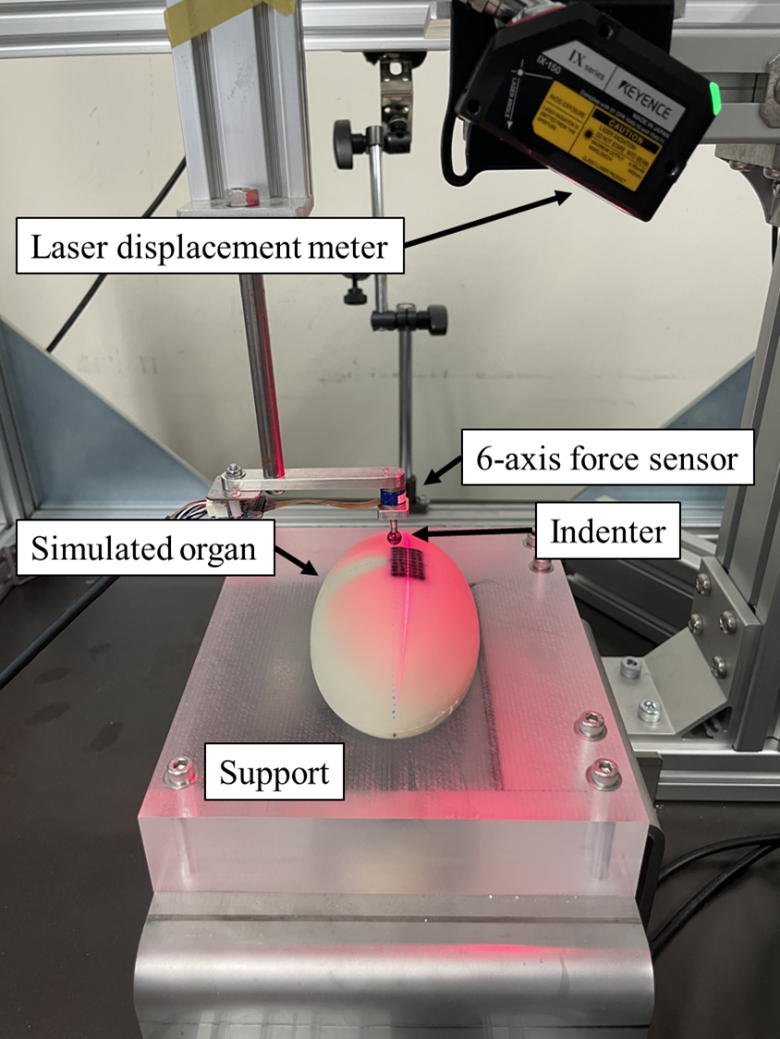
\includegraphics[width=10cm]{Images/appendix/ynu/fig1experimentaldevice.png}%
   \caption{Experimental device}%
   \label{fig:expdeviceynu}%
\end{figure}

\subsection*{Experimental Procedure}
The simulated organ to be loaded is shown in Figure \ref{fig:simorganynu} and a schematic diagram (top view) representing the coordinates of the loading points is shown in 
Figure \ref{fig:schemdiagynu}.
The loading points were set on the dotted line in Figure \ref{fig:schemdiagynu} because it was considered more suitable for parameter fitting if there were reaction forces of components other than the loading direction when performing the inverse analysis. The loading points were set at the top of the simulated organ and at a total of five points along the dotted line in
Figure \ref{fig:schemdiagynu}, moving with increments of $(\Delta X, \Delta Y) = (+2.5\,\mathrm{mm}, +2.5\,\mathrm{mm})$.\\
\begin{figure}%
	\centering
   \quad
   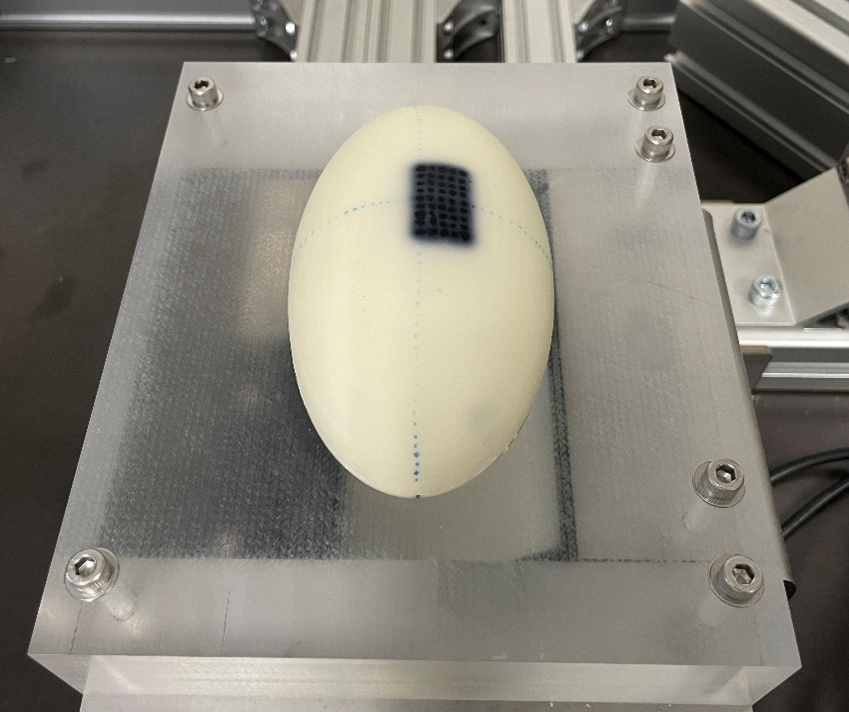
\includegraphics[width=10cm]{Images/appendix/ynu/fig2simulatedorgan.png}%
   \caption{Simulated organ}%
   \label{fig:simorganynu}%
\end{figure}
\begin{figure}%
	\centering
   \quad
   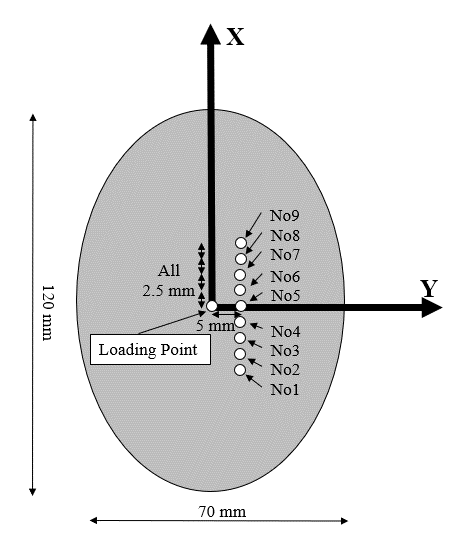
\includegraphics[width=8cm]{Images/appendix/ynu/fig3schematicdiagramrepresentingcoordinatesofloadingpoints_topview.png}%
   \caption[Schematic diagram YNU]{Schematic diagram representing coordinates of loading points (top view)}%
   \label{fig:schemdiagynu}%
\end{figure}

The experimental procedure is described below.
\begin{enumerate}
    \item Set the simulated organ on the table.
    \item Lubricate the loading point to eliminate the effect of friction.
    \item Move the measuring element directly above the loading point.
    \item Execute the G-code and start measuring the stroke, reaction force, and deformation.
    \item After the G-code is completed, terminate the measurement.
    \item Perform the same experiment 5 times for each loading point to confirm reproducibility.
\end{enumerate}

Experiments were conducted under room temperature environment (approx. \SI{20}{\degreeCelsius}).
The loading speed was \SI[per-mode = symbol]{30}{\milli \m\per \minute}, assuming the actual environment. 

\subsection*{Measurement method}
\subsubsection*{Measurement of indentation}
A $\SI{4}{\milli \m}$ load was applied to each loading point. The G code used in this study was designed to output a trigger voltage at a total of \SI{81}{}
times, and once when the bar was pushed in $\SI{0.1}{\milli \m}$.

These voltage changes were time-stamped using NI's USB-6003 and DAQ Express software. The indentation depth at the time of contact was set to
$\SI{0}{\milli \m}$, and the amount of indentation depth was measured as $\SI{0.1}{\milli \m}$ for each time the trigger voltage was transmitted. The sampling frequency was 
$\SI{10}{\kilo \hertz}$. An example of the voltage change during loading is shown in Figure \ref{fig:timevoltageynu}.\\
\begin{figure}%
	\centering
   \quad
   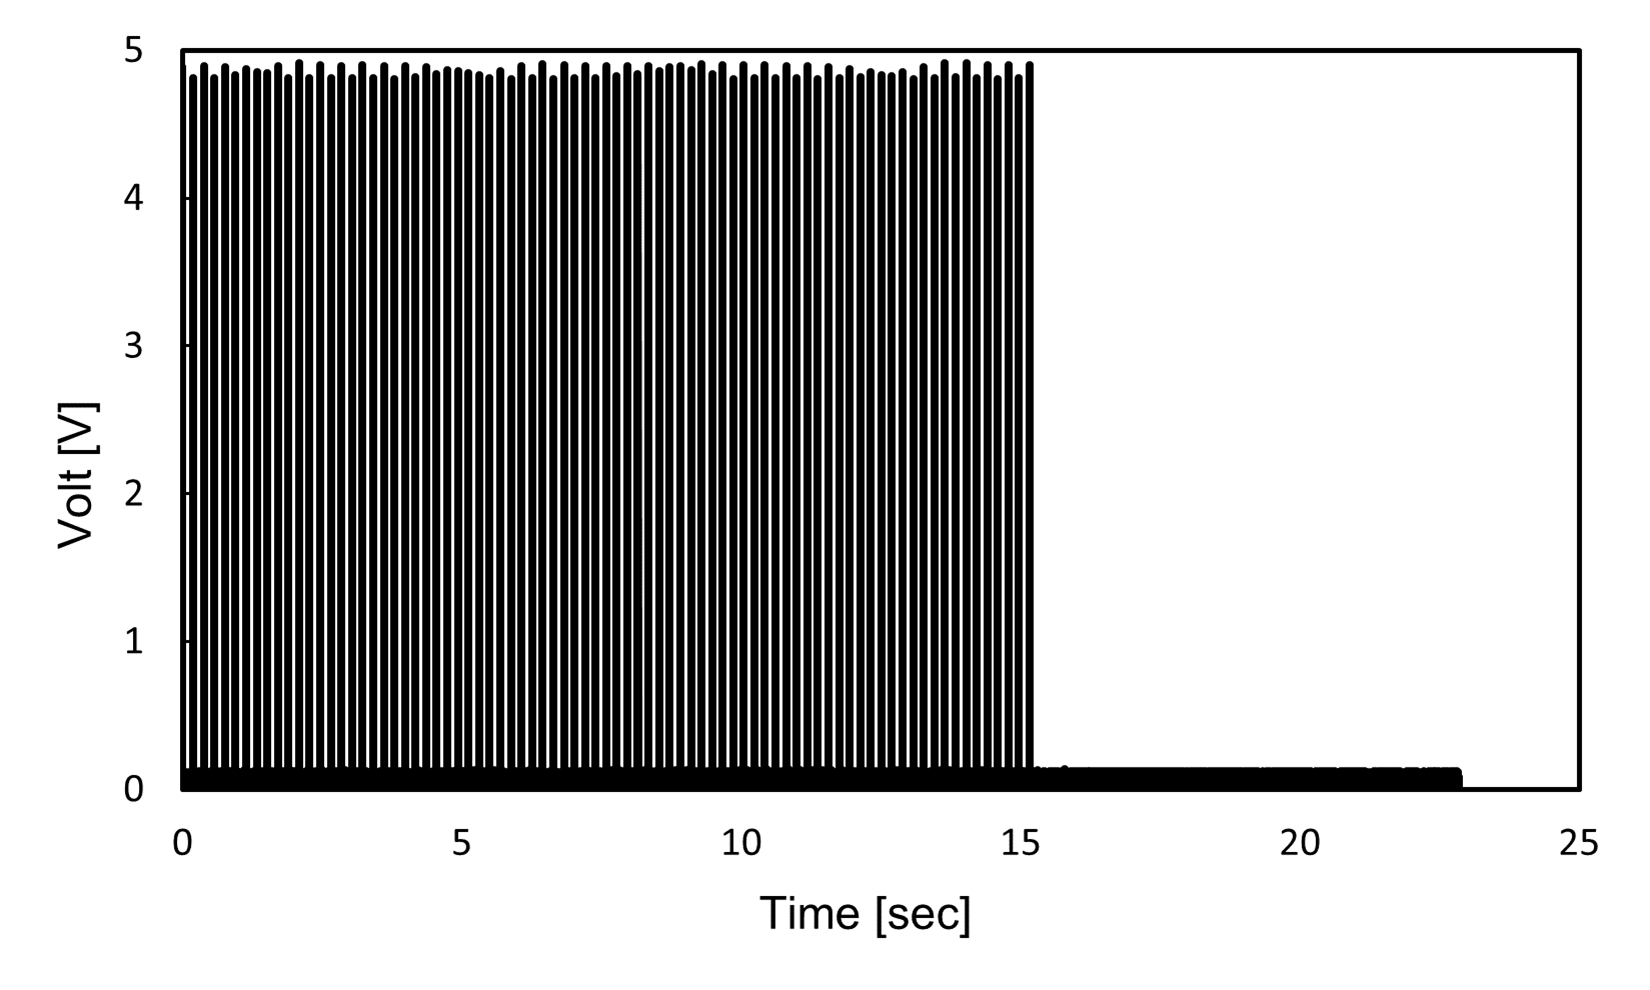
\includegraphics[width=10cm]{Images/appendix/ynu/fig4timehistoryoftriggervoltage.png}%
   \caption{Time history of trigger voltage}%
   \label{fig:timevoltageynu}%
\end{figure}
Because the reaction force and voltage were measured independently, the time axis was aligned by matching the peak time of the reaction force in the loading direction and the peak time of the push-in amount (Time when $\SI{4}{\milli \m}$ indented).

\subsubsection*{Measurement of reaction forces}
The specifications of the compact 6-axis force sensors are shown in Figure \ref{fig:specsensorynu}. 
\begin{figure}%
	\centering
   \quad
   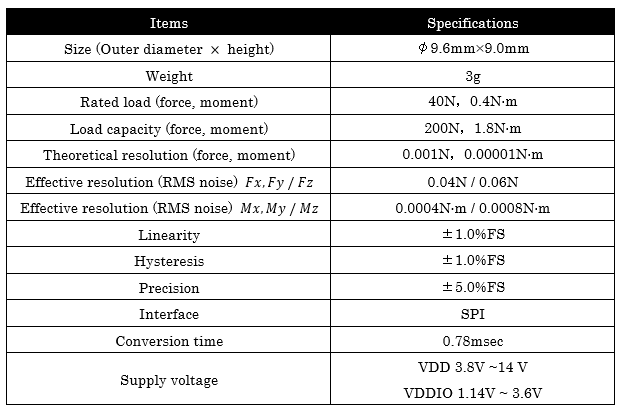
\includegraphics[width=10cm]{Images/appendix/ynu/tab1specificationsofminiature6axisforcesensors.png}%
   \caption{Specifications of miniature 6-axis force sensors}%
   \label{fig:specsensorynu}%
\end{figure}
The sampling frequency was $\SI{1000}{\hertz}$. To reduce the effect of initial drift, we waited five minutes to stabilize after sensor startup.

\subsubsection*{Measurement of deformation}
Figure \ref{fig:defmeasureynu} shows the laser beam on a straight line. Since the laser displacement meter was run with the same trigger voltage as the stroke measurement, the time when the deformation was measured was based on the time axis of the stroke.
\begin{figure}%
	\centering
   \quad
   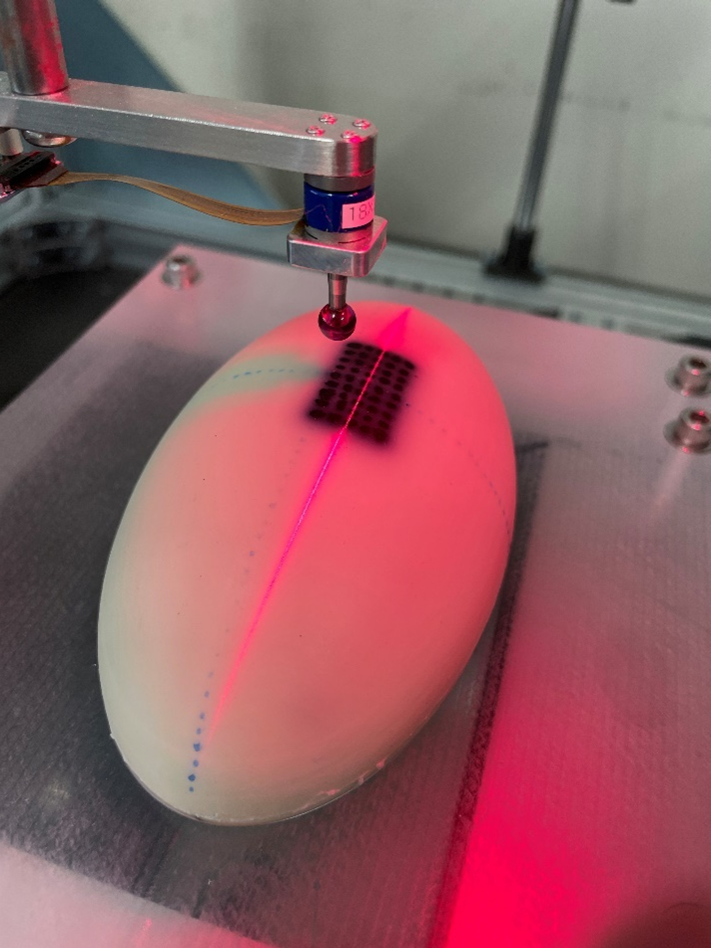
\includegraphics[width=8cm]{Images/appendix/ynu/fig5laserlineonthesimulatedorgan.png}%
   \caption{Deformation measurement}%
   \label{fig:defmeasureynu}%
\end{figure}

\subsection*{Experimental results}
The time history of the reaction force in the loading direction when the top of the simulated organ is loaded is shown 
in Figure \ref{fig:forcemeasurementynu}, and the deformation is shown in Figure \ref{fig:defmeasurementynu}. 
We performed five loading experiments to ensure reproducibility. The measurement accuracy of the laser displacement meter is
$\SI{0.05}{\milli \m}$.

The experimental results show that the deformation of the simulated organ at symmetrically located points, such as measurement points No. \SI{4}{} and No. \SI{6}{} (Fig. \ref{fig:disstroke}), are in good agreement with the results obtained by the laser displacement meter. The results indicate the possibility of using the deformation state obtained by laser displacement meter for the identification of physical properties in the future.
\begin{figure}
    \centering
    \begin{subfigure}[b]{0.45\textwidth}
    \centering
    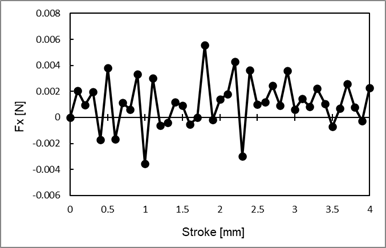
\includegraphics[width=\textwidth]{Images/appendix/ynu/fig6forcestroke_a.png}
    \caption{Force component in x-direction}
    \label{fig:forcezxnu}
    \end{subfigure}
    \hfill
    \begin{subfigure}[b]{0.45\textwidth}
    \centering
    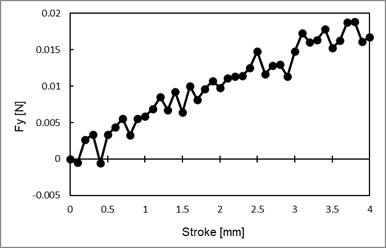
\includegraphics[width=\textwidth]{Images/appendix/ynu/fig6forcestroke_b.png}
    \caption{Force component in y-direction}
    \label{fig:forceyynu}
    \end{subfigure}
    \vspace{0.5cm}
    \begin{subfigure}[b]{0.45\textwidth}
    \centering
    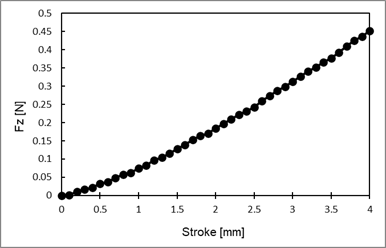
\includegraphics[width=\textwidth]{Images/appendix/ynu/fig6forcestroke_c.png}
    \caption{Force component in z-direction}
    \label{fig:forcezynu}
    \end{subfigure}  
    \hspace{0.3cm}
    \caption{Reaction force components results}
    \label{fig:forcemeasurementynu}
\end{figure}

\begin{figure}
    \centering
    \begin{subfigure}[b]{0.5\textwidth}
    \centering
    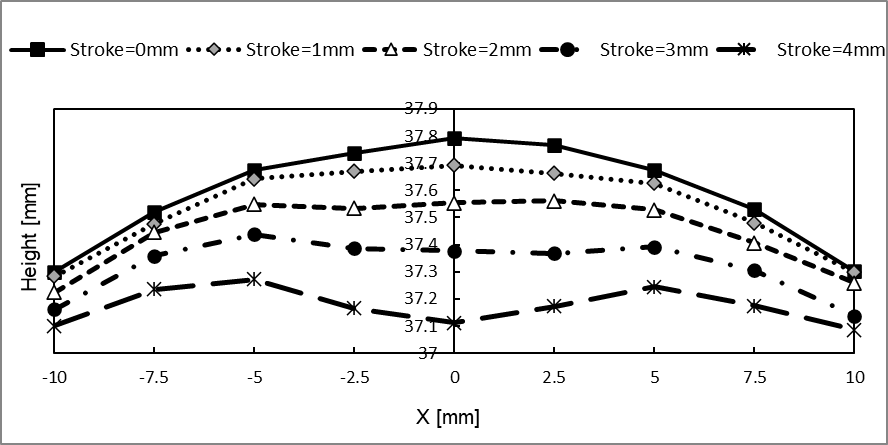
\includegraphics[width=\textwidth]{Images/appendix/ynu/fig7hightprofiletransition.png}
    \caption{Height profile transition}
    \label{fig:heighttrans}
    \end{subfigure}
    \hfill
    \begin{subfigure}[b]{0.5\textwidth}
    \centering
    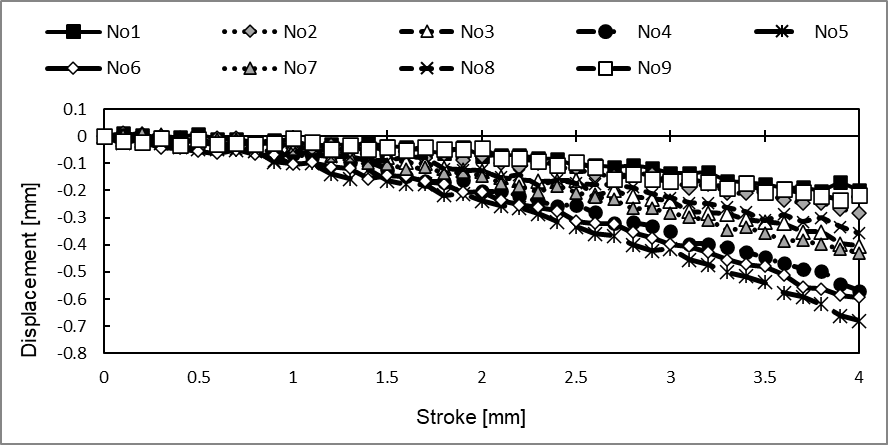
\includegraphics[width=\textwidth]{Images/appendix/ynu/fig8displacementsstroke.png}
    \caption{Displacement stroke}
    \label{fig:disstroke}
    \end{subfigure}
    \vspace{0.5cm}
    \caption{Deformation results}
    \label{fig:defmeasurementynu}
\end{figure}

%-----------------------------------------------------
\section{MATLAB Code}
\subsection*{NRMSE Polynomial Second Degree}

\lstset{style=matlab} % set the style to MATLAB
\begin{lstlisting}
   %Variables
   Mu = ...
   [0.0085415 0.012453 0.0099752 0.0099604 0.0099896 0.012315 0.0099752 0.0078715 0.0078906 0.007927 0.006500 0.006819 0.007153 0.007872 0.008258 0.008662 0.009087 0.009533 0.01 0.0099988 0.0099991 0.0099997 0.015 0.012 0.012 0.010867 0.010894 0.01092 0.0122 0.0132 0.0142 0.0122 0.0115 0.0142 0.0099 0.0098 0.0097 0.0101];
  
  D_1 = ...
   [5.25 139.31 127.51 127.8 128.6 131.62 5.25 1.0085 1.0085 4.1115 1 1 5 5 10 10 80 80 160 5.8429 5.8262 5.7867 50 50 1 47.199 48.454 49.677 72.8369 1.0017 1 159.683 1.002 101.3 50 50 50 50];
  
  NRMSE = ...
   [0.175 0.065 0.226 0.228 0.229 0.064 0.034 0.249 0.248 0.248 0.437 0.381 0.343 0.255 0.218 0.169 0.235 0.193 0.268 0.0339 0.0342 0.0339 0.4106 0.1197 0.2659 0.0343 0.0351 0.0352 0.08339 0.41757 0.539562 0.09984 0.20519 0.17806 0.103 0.114 0.124 0.0844];
  
  X = transpose([Mu; D_1]);
  y = NRMSE;
  
  %Polynomial degree 2
         p00 =       2.798;
         p10 =        -535;
         p01 =    0.009251;
         p20 =   2.654e+04;
         p11 =      -1.022;
         p02 =   1.467e-05;
  f = @(x) (p00 + p10*x(1) + p01*x(2) + p20*x(1)^2 + p11*x(1)*x(2) + p02*x(2)^2);
  
  %Setting the upper and lower boundaries
  lb = [0.0001, 1];
  ub = [1, 1000];

  %Finding the minimum
  [xmin,FVAL] = fmincon(f, [0.012453, 139.31], [], [], [], [], lb, ub);
\end{lstlisting}

\subsection*{MRE Polynomial Fourth Degree}

\lstset{style=matlab} % set the style to MATLAB

\begin{lstlisting}
%Variables
Mu = ...
 [0.0085415 0.012453 0.0099752 0.0099604 0.0099896 0.012315 0.0099752 0.0078715 0.0078906 0.007927 0.0065 0.006819 0.007153 0.007872 0.008258 0.008662 0.009087 0.009533 0.01 0.0099988 0.0099991 0.0099997 0.015 0.012 0.012 0.010867 0.010894 0.01092 0.0122 0.0132 0.0142 0.0122 0.0115 0.0142 0.0099 0.0098 0.0097 0.0101 0.0122 0.0119 0.0101 0.0099 0.0105];

D_1 = ...
 [5.25 139.31 127.51 127.8 128.6 131.62 5.25 1.0085 1.0085 4.1115 1 1 5 5 10 10 80 80 160 5.8429 5.8262 5.7867 50 50 1 47.199 48.454 49.677 72.8369 1.0017 1 153.68 1.002 101.3 50 50 50 50 108.66 72.7 5.5 5.5 5.5];

MRE = ...
 [0.2188 0.1713 0.2916 0.2928 0.2929 0.1697 0.1098 0.273 0.2715 0.2726 0.4153 0.3706 0.3444 0.2786 0.253 0.2175 0.288 0.2588 0.3241 0.1103 0.1104 0.1098 0.2831 0.1479 0.2183 0.1207 0.1219 0.1218 0.1388 0.3086 0.386 0.2012 0.1847 0.1717 0.1838 0.1914 0.1983 0.1689 0.1429 0.1331 0.1111 0.1105 0.125];

X = transpose([Mu; D_1]);
y = MRE;

%Polynomial degree 4
p00 =      -6.509;
p10 =        3317;
p01 =    -0.07093;
p20 =  -5.609e+05;
p11 =       23.91;
p02 =  -0.0003905;
p30 =   3.927e+07;
p21 =       -2470;
p12 =     0.07195;
p03 =  -2.663e-07;
p40 =  -9.728e+08;
p31 =   7.912e+04;
p22 =      -3.035;
p13 =   8.145e-06; 
p04 =    4.08e-10;

f =  @(x) (p00 + p10*x(1) + p01*x(2) + p20*x(1)^2 + p11*x(1)*x(2) + p02*x(2)^2 + p30*x(1)^3 + p21*x(1)^2*x(2) + p12*x(1)*x(2)^2 + p03*x(2)^3 + p40*x(1)^4 + p31*x(1)^3*x(2) + p22*x(1)^2*x(2)^2 + p13*x(1)*x(2)^3 + p04*x(2)^4);

%Setting the upper and lower boundaries
lb = [0.007, 0.1];
ub = [0.013, 100];

%Finding the minimum
[xmin,FVAL] = fmincon(f, [0.012453, 139.31], [], [], [], [], lb, ub);

x = linspace(0.0001, 0.1, 20);
y = linspace(5,1000, 20);
\end{lstlisting}

% Bibliography
\printbibliography[heading=bibintoc]



\end{document}  
